%\documentclass[11pt,a4paper]{article}
\documentclass[12pt,a4paper]{scrartcl}
%\documentclass[11pt,a4paper,oneside]{book}
\ifdefined\PWRCONTROLSETTINGSLOADED
\endinput
\fi
\def\PWRCONTROLSETTINGSLOADED{1}
% ===================== PACKAGES =====================
\usepackage[british]{babel}
\usepackage[tmargin=1in, bmargin=1in, lmargin=0.75in, rmargin=0.75in]{geometry}
\usepackage[dvipsnames,table]{xcolor}  % prima di tikz, listings, ecc.

\usepackage{tikz}
\usepackage{graphicx}
\usepackage{pgfplots}
\pgfplotsset{width=12cm, compat=1.9}
\usepackage{setspace}
\usepackage{chemmacros}
\usepackage{chemfig}
\usepackage{tabularray}
\usepackage{makeidx}
\usepackage{epstopdf}
\usepackage{amssymb}
\usepackage{mathrsfs}
\usepackage{bm}
\usepackage{amsmath}
% esint deve essere caricato DOPO amsmath: entrambi definiscono \iint, \iiint,
% \iiiint e \idotsint. Le si rende indefinite in modo che esint le ridefinisca
% (versioni con i simboli di integrale multiplo corretti) senza errori.
\let\iint\undefined
\let\iiint\undefined
\let\iiiint\undefined
\let\idotsint\undefined
\usepackage{esint}
\usepackage{enumitem}
%\usepackage[english]{varioref}
\usepackage{physics}
\usepackage{lipsum}
\usepackage{fancyhdr}
\usepackage{float}
\usepackage{empheq}
\usepackage[framemethod=tikz]{mdframed}
\numberwithin{equation}{section}
\usepackage{eso-pic}
\usepackage{calc}
\usepackage{nccmath}
\usepackage{caption}
\usepackage{subcaption}
\usepackage{gensymb}
\usepackage{amsfonts, amsthm, epsfig, epstopdf, titling, url, array}
\usepackage{tabularx}
\usepackage{makecell}
\usepackage{booktabs}
\usepackage{array}
\usepackage{siunitx}
\sisetup{input-digits=0123456789\pi}
\usepackage[symbol]{footmisc}
\usepackage{multicol}
%\usepackage{boondox-cal}
\usepackage{blindtext}
\usepackage{changepage}
\usepackage{nomencl}
\usepackage{hyperref}
\usepackage{xurl}
\usepackage{ragged2e}
\usepackage[version=4]{mhchem}  % ← conflitto di opzioni
\usepackage{longtable}
\usepackage{chemformula}
\usetikzlibrary{arrows.meta,positioning,calc}
\usepackage[page,toc]{appendix}


% ===================== SI UNITS =====================
\DeclareSIUnit\atm{atm}
\DeclareSIUnit{\var}{var}
\DeclareSIUnit{\pu}{p.u.}
\sisetup{detect-weight=true, detect-inline-weight=math}

% ===================== MATH OPERATORS =====================
%\DeclareMathOperator{\rank}{rank}
\DeclareMathOperator{\atantwo}{atan2}
\DeclareMathOperator{\spn}{span}

% ===================== COMMANDS =====================
%\newcommand{\abs}[1]{\left|#1\right|}
\newcommand{\sign}{\text{sign}}
\newcommand{\centered}[1]{\begin{tabular}{@{}l@{}} #1 \end{tabular}}

% ===================== COLORS =====================
\definecolor{mycolor1}{rgb}{0.97, 0.97, 0.97}
\definecolor{mycolor2}{rgb}{0.97, 0.97, 0.97}
\definecolor{tableShade}{gray}{0.9}

% ===================== THEOREM ENVIRONMENTS =====================
\theoremstyle{it}
\newtheorem{defn}{Definition}[section]
\newtheorem{assumption}{Assumption}[section]
\newtheorem{thm}{Theorem}[section]
\newtheorem{lemma}{Lemma}[section]
\newtheorem{corollary}{Corollary}[section]
\theoremstyle{definition}
\newtheorem{example}{Example}[section]

% ===================== CUSTOM ENVIRONMENTS =====================
\newenvironment{myitemize_1}{
	\begin{itemize}[topsep=0pt]
		\setlength{\topsep}{2pt}
		\setlength{\itemsep}{2pt}
		\setlength{\parskip}{2pt}
		\setlength{\parsep}{2pt}
	}{\end{itemize}}

\newmdenv[
innerlinewidth=0.5pt,
roundcorner=4pt,
backgroundcolor=mycolor2,
linecolor=mycolor1,
innerleftmargin=6pt,
innerrightmargin=6pt,
innertopmargin=6pt,
innerbottommargin=6pt
]{mybox}

% ===================== TABLE COLUMN TYPES =====================
\newcolumntype{Y}{>{\hsize=2\hsize}X}
\newcolumntype{Z}{>{\centering\arraybackslash\hsize=0.857\hsize}X}

% ===================== SECTION DEPTH =====================
\setcounter{secnumdepth}{3}
\setcounter{tocdepth}{3}

% ===================== PAGE STYLE =====================
\setlength{\headheight}{20pt}
\setlength{\headsep}{20pt}

\pagestyle{fancy}
\fancypagestyle{firstpage}{\rhead{}}
\fancyhead[L]{\slshape\nouppercase{\leftmark}}
\chead{}
\rhead{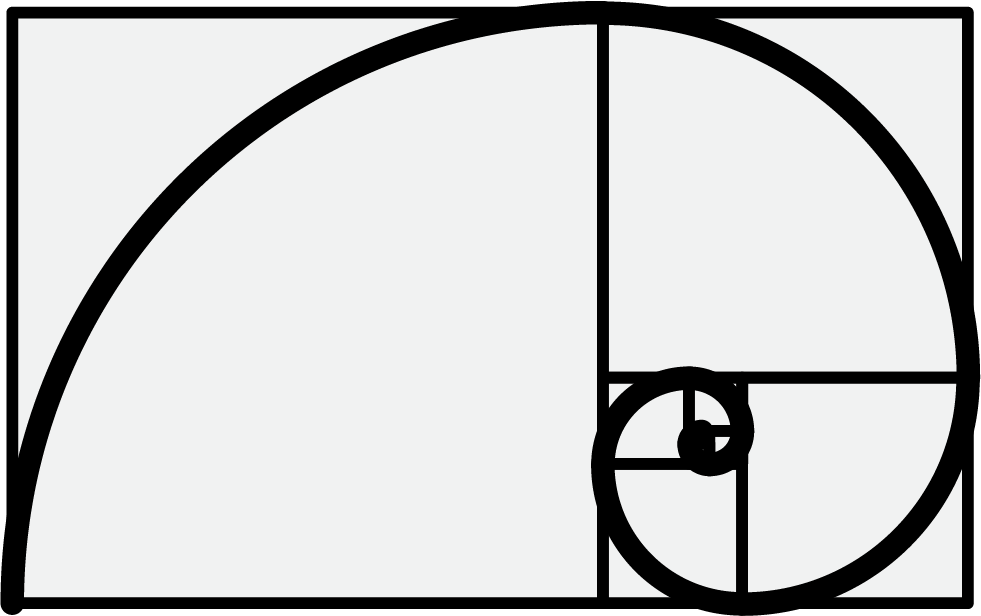
\includegraphics[height=0.75cm]{../../AAA_template_latex_settings/pwr-control_logo_doc.png}}
\lfoot{\href{https://github.com/pwr-control}{\color{black} pwr-control}}
\cfoot{-\ \thepage\ -}
\rfoot{\textit{}}
\renewcommand{\headrulewidth}{0.4pt}
\renewcommand{\footrulewidth}{0.4pt}


\geometry{
	a4paper,
	top    = 2.5cm,
	bottom = 3.0cm,
	left   = 2.5cm,
	right  = 2.5cm
}

\hypersetup{
	colorlinks = true,
	urlcolor   = blue,
	linkcolor  = black,
	citecolor  = black
}

\pagenumbering{gobble}



% =============================================================
%  DOCUMENT METADATA
% =============================================================

\newcommand{\DocCategory}{Technical Research Report}
\newcommand{\DocField}{Power Electronics and Control Systems}

\newcommand{\DocTitle}{%
	{\fontsize{20}{24}\selectfont\bfseries Solid State Transformers:} \\[16pt]
	{\fontsize{16}{20}\selectfont\bfseries architecture, modelization and control.}
}

\newcommand{\DocSubtitle}{%
	Investigation on different layouts based on DAB, DAB3 and CLLC, and the two-module bench built on the CLLC-DCX and the T-type inverter.
}

\newcommand{\DocAuthor}{Davide Bagnara}
\newcommand{\DocRevision}{01}
\newcommand{\DocDate}{October 2026}

\newcommand{\DocAbstract}{%
	A solid state transformer (\textit{SST}) replaces the line frequency transformer of a distribution system with a chain of high frequency isolated power electronic stages, gaining compactness, efficiency and control over the power flow, the voltage and the reactive power; its inherent current limiting, on the other hand, deprives the downstream overcurrent protections of the fault current they rely upon. This document is a preliminary comparative investigation of \textit{SST} architectures placed between a low voltage DC grid and a three phase medium voltage AC grid. The proposed layout is a cascade of series connected single phase inverters, each one supplied by its own galvanically isolated DC/DC converter with the inputs connected in parallel, operated in a master/slave arrangement in which every unit runs its own single phase \textit{PLL}. Three isolated DC/DC stages are compared --- three phase DAB, single phase DAB and single phase bidirectional CLLC --- together with two inverter topologies, three level NPC and three level T-type, built with Wolfspeed SiC modules. The control architecture is described and each combination is simulated in \textit{Simscape} at about \SI{250}{\kilo\watt} per phase, with the semiconductor losses collected and compared. A dedicated chapter covers the design of the high frequency transformers of the three phase DAB and of the single phase DAB, on nanocrystalline C-cores with copper foil windings. The last chapter, added in this revision, documents the bench that the repository keeps today: two \SI{50}{\kilo\watt} modules, each one a CLLC resonant converter run as an open-loop DC transformer (\SI{800}{\volt} to \SI{800}{\volt}, \SI{50}{\kilo\hertz}) feeding a three level T-type single phase inverter, with the two inverters in series on the line; its structure, control, parameter organization and numerical settings are described, together with the two compact library blocks that model one DCX and one inverter each in two nonvirtual blocks.
}

% Righe della revision history: Rev. & Date & Description & Authors \\
\newcommand{\RevisionHistory}{%
	00 & May 2025 & First issue. & \DocAuthor \\
	01 & October 2026 & Two-module CLLC-DCX / T-type bench of the repository (Section~\ref{sec:bench2026}), state of the repository and references to the CLLC-DCX and single phase inverter notes; figure paths without extension. & \DocAuthor \\
}

% Metadati in fondo al frontespizio
\newcommand{\MetaLabelA}{Project Repository}
\newcommand{\MetaValueAUrl}{https://github.com/pwr-control/solid-state-transformers.git}
\newcommand{\MetaValueALabel}{solid-state-transformers.git}

\newcommand{\MetaLabelB}{Framework}
\newcommand{\MetaValueB}{MATLAB/Simulink/Simscape}

% =============================================================
%  DOCUMENTO
% =============================================================
\begin{document}
	% =============================================================
%  pwr-control LaTeX template - FRONTESPIZIO
%
%  Da richiamare come prima istruzione dopo \begin{document}:
%      % =============================================================
%  pwr-control LaTeX template - FRONTESPIZIO
%
%  Da richiamare come prima istruzione dopo \begin{document}:
%      % =============================================================
%  pwr-control LaTeX template - FRONTESPIZIO
%
%  Da richiamare come prima istruzione dopo \begin{document}:
%      \input{../../AAA_template_latex_settings/titlepage}
%
%  Il documento deve definire prima di \begin{document}:
%      \DocCategory   categoria del documento
%      \DocField      area tecnica
%      \DocTitle      titolo (una o due righe)
%      \DocSubtitle   sottotitolo
%      \DocAuthor     autore/i, separati da virgola
%      \DocRevision   numero di revisione corrente (es. 00)
%      \DocDate       data della revisione corrente
%      \DocAbstract   abstract
%      \RevisionHistory  righe della tabella di revisione, nel formato
%                        Rev. & Date & Description & Authors \\
%      \MetaLabelA \MetaValueAUrl \MetaValueALabel
%      \MetaLabelB \MetaValueB
% =============================================================

\providecommand{\DocCategory}{Technical Research Report}
\providecommand{\DocField}{Power Electronics and Control Systems}
\providecommand{\DocSubtitle}{}
\providecommand{\DocRevision}{00}
\providecommand{\DocAbstract}{}
\providecommand{\RevisionHistory}{%
	\DocRevision & \DocDate & First issue. & \DocAuthor \\
}

\titlepage

% ---- Intestazione centrata ----
\begin{center}
	{\Large\scshape \DocCategory}\\[8pt]
	{\large\scshape \DocField}
\end{center}

\vspace{30pt plus 4pt minus 14pt}
\noindent\rule{\linewidth}{0.8pt}

% ---- Titolo ----
\begin{center}
	\DocTitle
\end{center}

\vspace{4pt}
\noindent\rule{\linewidth}{2.2pt}

% ---- Sottotitolo ----
\begin{center}
	\begin{onehalfspace}
		{\large\itshape \DocSubtitle}
	\end{onehalfspace}
\end{center}

% ---- Authors / Revision / Date ----
\vspace{30pt plus 4pt minus 14pt}

\noindent
\begin{minipage}[t]{0.46\linewidth}
	\raggedright
	\textbf{Authors:}\\[2pt]
	\DocAuthor
\end{minipage}%
\hfill
\begin{minipage}[t]{0.22\linewidth}
	\centering
	\textbf{Revision:}\\[2pt]
	\DocRevision
\end{minipage}%
\hfill
\begin{minipage}[t]{0.30\linewidth}
	\raggedleft
	\textbf{Date:}\\[2pt]
	\DocDate
\end{minipage}

\vspace{10pt}
\noindent\rule{\linewidth}{0.8pt}

% ---- Abstract ----
\vspace{24pt plus 4pt minus 12pt}

\begin{center}
	\begin{minipage}{0.88\linewidth}
		\footnotesize
		\begin{onehalfspace}
			\textbf{Abstract:} \DocAbstract
		\end{onehalfspace}
	\end{minipage}
\end{center}

\vfill

% ---- Revision history ----
\begin{center}
	\begin{minipage}{0.96\linewidth}
		\centering
		{\footnotesize\scshape Revision history}\\[6pt]
		{\footnotesize
			\begin{tabular}{@{}cl>{\raggedright\arraybackslash}p{0.36\linewidth}>{\raggedright\arraybackslash}p{0.28\linewidth}@{}}
				\toprule
				\textbf{Rev.} & \textbf{Date} & \textbf{Description} & \textbf{Authors} \\
				\midrule
				\RevisionHistory
				\bottomrule
			\end{tabular}}
	\end{minipage}
\end{center}

\vspace{18pt plus 4pt minus 10pt}

% ---- Metadati in fondo ----
\noindent
\begin{tabular}{@{} r @{\quad} l @{}}
	\textsc{\MetaLabelA:} & {\href{\MetaValueAUrl}{\MetaValueALabel}} \\[3pt]
	\textsc{\MetaLabelB:} & {\MetaValueB}       \\[3pt]
\end{tabular}

% =============================================================
%  Fine frontespizio
% =============================================================
\newpage
\pagenumbering{arabic}
\setcounter{page}{1}

%
%  Il documento deve definire prima di \begin{document}:
%      \DocCategory   categoria del documento
%      \DocField      area tecnica
%      \DocTitle      titolo (una o due righe)
%      \DocSubtitle   sottotitolo
%      \DocAuthor     autore/i, separati da virgola
%      \DocRevision   numero di revisione corrente (es. 00)
%      \DocDate       data della revisione corrente
%      \DocAbstract   abstract
%      \RevisionHistory  righe della tabella di revisione, nel formato
%                        Rev. & Date & Description & Authors \\
%      \MetaLabelA \MetaValueAUrl \MetaValueALabel
%      \MetaLabelB \MetaValueB
% =============================================================

\providecommand{\DocCategory}{Technical Research Report}
\providecommand{\DocField}{Power Electronics and Control Systems}
\providecommand{\DocSubtitle}{}
\providecommand{\DocRevision}{00}
\providecommand{\DocAbstract}{}
\providecommand{\RevisionHistory}{%
	\DocRevision & \DocDate & First issue. & \DocAuthor \\
}

\titlepage

% ---- Intestazione centrata ----
\begin{center}
	{\Large\scshape \DocCategory}\\[8pt]
	{\large\scshape \DocField}
\end{center}

\vspace{30pt plus 4pt minus 14pt}
\noindent\rule{\linewidth}{0.8pt}

% ---- Titolo ----
\begin{center}
	\DocTitle
\end{center}

\vspace{4pt}
\noindent\rule{\linewidth}{2.2pt}

% ---- Sottotitolo ----
\begin{center}
	\begin{onehalfspace}
		{\large\itshape \DocSubtitle}
	\end{onehalfspace}
\end{center}

% ---- Authors / Revision / Date ----
\vspace{30pt plus 4pt minus 14pt}

\noindent
\begin{minipage}[t]{0.46\linewidth}
	\raggedright
	\textbf{Authors:}\\[2pt]
	\DocAuthor
\end{minipage}%
\hfill
\begin{minipage}[t]{0.22\linewidth}
	\centering
	\textbf{Revision:}\\[2pt]
	\DocRevision
\end{minipage}%
\hfill
\begin{minipage}[t]{0.30\linewidth}
	\raggedleft
	\textbf{Date:}\\[2pt]
	\DocDate
\end{minipage}

\vspace{10pt}
\noindent\rule{\linewidth}{0.8pt}

% ---- Abstract ----
\vspace{24pt plus 4pt minus 12pt}

\begin{center}
	\begin{minipage}{0.88\linewidth}
		\footnotesize
		\begin{onehalfspace}
			\textbf{Abstract:} \DocAbstract
		\end{onehalfspace}
	\end{minipage}
\end{center}

\vfill

% ---- Revision history ----
\begin{center}
	\begin{minipage}{0.96\linewidth}
		\centering
		{\footnotesize\scshape Revision history}\\[6pt]
		{\footnotesize
			\begin{tabular}{@{}cl>{\raggedright\arraybackslash}p{0.36\linewidth}>{\raggedright\arraybackslash}p{0.28\linewidth}@{}}
				\toprule
				\textbf{Rev.} & \textbf{Date} & \textbf{Description} & \textbf{Authors} \\
				\midrule
				\RevisionHistory
				\bottomrule
			\end{tabular}}
	\end{minipage}
\end{center}

\vspace{18pt plus 4pt minus 10pt}

% ---- Metadati in fondo ----
\noindent
\begin{tabular}{@{} r @{\quad} l @{}}
	\textsc{\MetaLabelA:} & {\href{\MetaValueAUrl}{\MetaValueALabel}} \\[3pt]
	\textsc{\MetaLabelB:} & {\MetaValueB}       \\[3pt]
\end{tabular}

% =============================================================
%  Fine frontespizio
% =============================================================
\newpage
\pagenumbering{arabic}
\setcounter{page}{1}

%
%  Il documento deve definire prima di \begin{document}:
%      \DocCategory   categoria del documento
%      \DocField      area tecnica
%      \DocTitle      titolo (una o due righe)
%      \DocSubtitle   sottotitolo
%      \DocAuthor     autore/i, separati da virgola
%      \DocRevision   numero di revisione corrente (es. 00)
%      \DocDate       data della revisione corrente
%      \DocAbstract   abstract
%      \RevisionHistory  righe della tabella di revisione, nel formato
%                        Rev. & Date & Description & Authors \\
%      \MetaLabelA \MetaValueAUrl \MetaValueALabel
%      \MetaLabelB \MetaValueB
% =============================================================

\providecommand{\DocCategory}{Technical Research Report}
\providecommand{\DocField}{Power Electronics and Control Systems}
\providecommand{\DocSubtitle}{}
\providecommand{\DocRevision}{00}
\providecommand{\DocAbstract}{}
\providecommand{\RevisionHistory}{%
	\DocRevision & \DocDate & First issue. & \DocAuthor \\
}

\titlepage

% ---- Intestazione centrata ----
\begin{center}
	{\Large\scshape \DocCategory}\\[8pt]
	{\large\scshape \DocField}
\end{center}

\vspace{30pt plus 4pt minus 14pt}
\noindent\rule{\linewidth}{0.8pt}

% ---- Titolo ----
\begin{center}
	\DocTitle
\end{center}

\vspace{4pt}
\noindent\rule{\linewidth}{2.2pt}

% ---- Sottotitolo ----
\begin{center}
	\begin{onehalfspace}
		{\large\itshape \DocSubtitle}
	\end{onehalfspace}
\end{center}

% ---- Authors / Revision / Date ----
\vspace{30pt plus 4pt minus 14pt}

\noindent
\begin{minipage}[t]{0.46\linewidth}
	\raggedright
	\textbf{Authors:}\\[2pt]
	\DocAuthor
\end{minipage}%
\hfill
\begin{minipage}[t]{0.22\linewidth}
	\centering
	\textbf{Revision:}\\[2pt]
	\DocRevision
\end{minipage}%
\hfill
\begin{minipage}[t]{0.30\linewidth}
	\raggedleft
	\textbf{Date:}\\[2pt]
	\DocDate
\end{minipage}

\vspace{10pt}
\noindent\rule{\linewidth}{0.8pt}

% ---- Abstract ----
\vspace{24pt plus 4pt minus 12pt}

\begin{center}
	\begin{minipage}{0.88\linewidth}
		\footnotesize
		\begin{onehalfspace}
			\textbf{Abstract:} \DocAbstract
		\end{onehalfspace}
	\end{minipage}
\end{center}

\vfill

% ---- Revision history ----
\begin{center}
	\begin{minipage}{0.96\linewidth}
		\centering
		{\footnotesize\scshape Revision history}\\[6pt]
		{\footnotesize
			\begin{tabular}{@{}cl>{\raggedright\arraybackslash}p{0.36\linewidth}>{\raggedright\arraybackslash}p{0.28\linewidth}@{}}
				\toprule
				\textbf{Rev.} & \textbf{Date} & \textbf{Description} & \textbf{Authors} \\
				\midrule
				\RevisionHistory
				\bottomrule
			\end{tabular}}
	\end{minipage}
\end{center}

\vspace{18pt plus 4pt minus 10pt}

% ---- Metadati in fondo ----
\noindent
\begin{tabular}{@{} r @{\quad} l @{}}
	\textsc{\MetaLabelA:} & {\href{\MetaValueAUrl}{\MetaValueALabel}} \\[3pt]
	\textsc{\MetaLabelB:} & {\MetaValueB}       \\[3pt]
\end{tabular}

% =============================================================
%  Fine frontespizio
% =============================================================
\newpage
\pagenumbering{arabic}
\setcounter{page}{1}

	\tableofcontents
	\listoffigures
	\listoftables
	\newpage

\begin{onehalfspace}
\section{Introduction}
\textbf{Solid State Transformers (SSTs)} are advanced power electronic devices designed to replace traditional low-frequency transformers in modern power distribution systems. By operating at high frequency and using fully controllable conversion stages, SSTs achieve a more compact size, improved energy efficiency, and enhanced functionality compared to conventional transformers. Beyond simple voltage transformation, they provide additional services such as bidirectional power flow, voltage and reactive power regulation, and seamless integration of distributed energy resources including renewables, electric vehicles, and energy storage.

A key difference from traditional transformers is the behavior of SSTs during fault conditions. Due to their electronic nature and active current limiting, SSTs inherently restrict short-circuit currents. This prevents downstream systems from relying on conventional overcurrent-based protection schemes, which depend on high fault currents for detection. As a result, new protection strategies based on advanced sensing, high-speed control, and intelligent fault identification must be implemented. This shift in protection philosophy presents both challenges and significant opportunities for the development of more flexible, reliable, and smart power networks.

\noindent\textbf{Structure of the document and state of the repository (Rev.~01).} Sections~\ref{sec:global_arch} to~\ref{sec:summary} are the comparative study of 2025: the candidate architectures, the control principles, the simulation of each combination of isolated DC/DC stage (three phase DAB, single phase DAB, single phase CLLC) and inverter (NPC, T-type) at about \SI{250}{\kilo\watt} per phase, the transformer designs and the comparison of the losses. They are kept as they were written; the models they refer to were removed from the tree of the repository \cite{sst_repo} in March 2026 (they remain in the git history), and the three phase DAB study continues in the \textit{advanced-dcdc-converters} repository. What the repository keeps today is a single two-module bench built on the outcome of the study, the single phase CLLC used as a DC transformer and the T-type inverter, at \SI{50}{\kilo\watt} per module and with the library blocks of \cite{library_repo}: Section~\ref{sec:bench2026} documents it. The isolated stage of that bench has its own design note \cite{cllc_dcx_doc}, and the single phase inverter with its control design the note \cite{spinv_doc}.

\section{Global Architecture}
\label{sec:global_arch}
In this chapter few general architectures for SST solutions are proposed and investigated; the SST device is intended to operate between two different grids:
\begin{itemize}
	\item[--] a low voltage DC grid source where many contributors can be assumed are connected e.g. energy storage, photovoltaic installations, car chargers and others;
	\item[--] a three phase medium voltage AC grid source;	 
\end{itemize} 

\noindent Figure~\ref{sst_design_ctrl_fig4b} shows a single phase architecture, which basically consists by a cascade of single phase inverters, where each single phase inverter is supplied by a galvanically isolated DC/DC converter. Each single phase inverter which constitute a single are all connected in series to achieve the selected AC medium voltage; on the other hand all DC/DC input stage are connected in parallel.

\noindent\textbf{Remark} - to reduce the stress in term of voltage isolation, the HV/MV transformer could be built in a way to equally distribute the phase to grand voltage, as shown in Figure~\ref{sst_design_ctrl_fig4b}.

\noindent\textbf{Remark} - from control point of view the following layout can be assumed:
\begin{itemize}
	\item[--] DC/DC power supply control is monolithic and atomic; 	
	\item[--] three phase active front end (AFE) control architecture can be assumed as follows
	\begin{itemize}
		\item[--] master/slave configuration: for each phase one single phase inverter will be identified as \textit{master} while \textit{slave} the others;		
		\item[--] each single phase inverter is equipped by a single phase PLL (both \textit{master} and \textit{slaves});
		\item[--] an inverter current control (running on \textit{master});		
		\item[--] a voltage controlled source mode (on \textit{slaves}).			
	\end{itemize}
\end{itemize}
\begin{figure}[H]
	\centering
	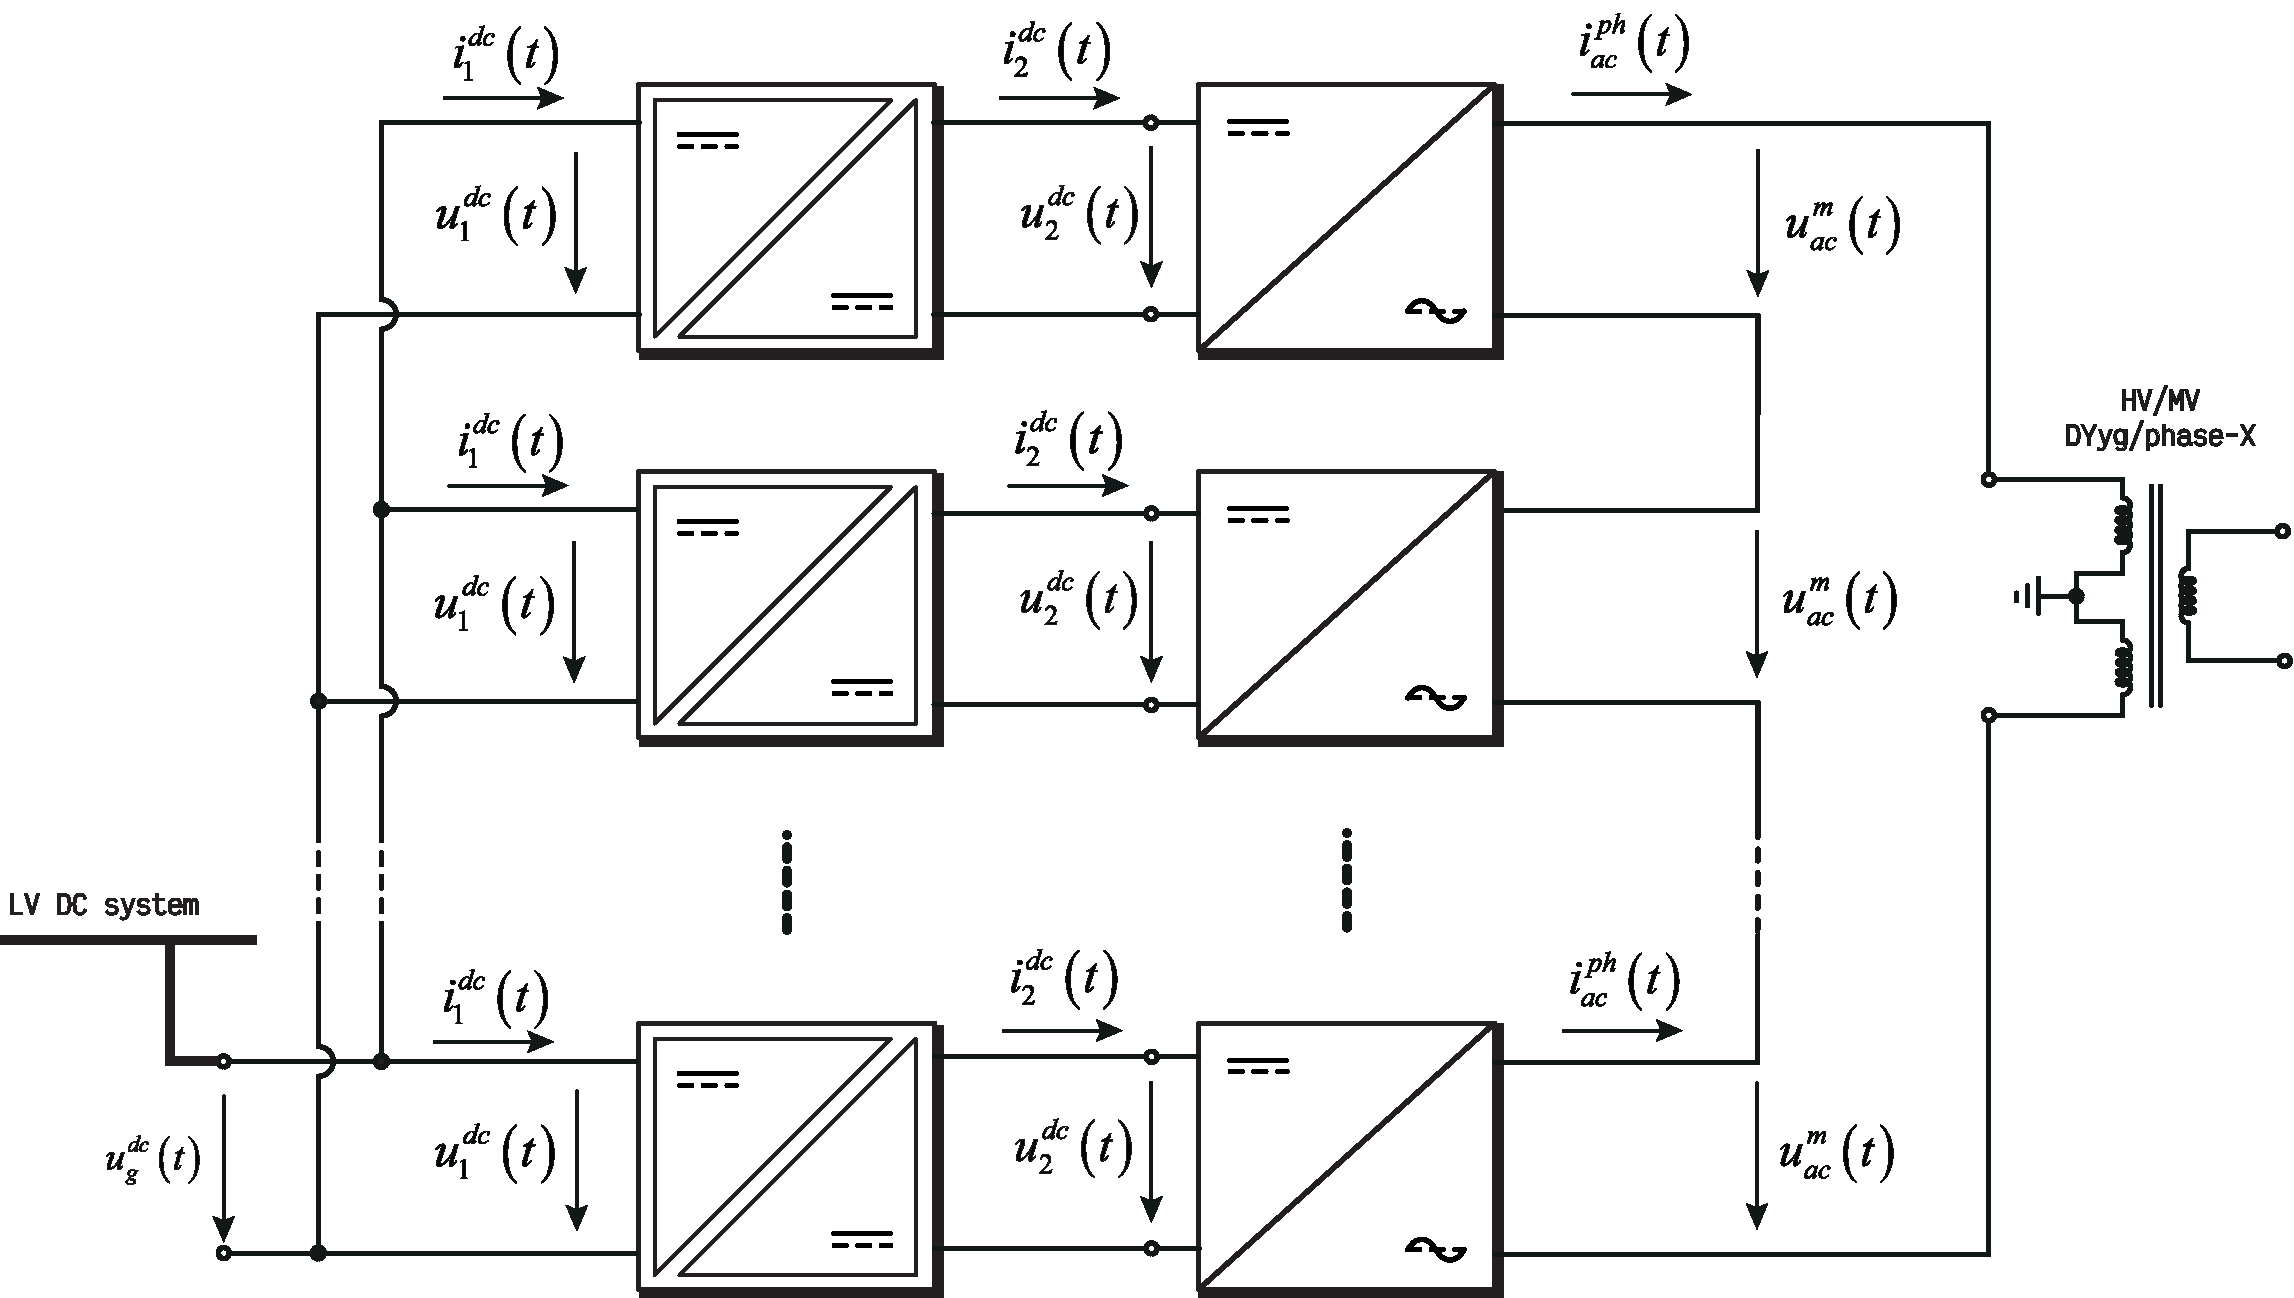
\includegraphics[width = 500pt, angle = 0, 
	keepaspectratio]{figures/arch/sst_design_ctrl_fig4b}
	\captionsetup{width=0.5\textwidth, font=small}
	\caption{Single phase architecture based on galvanically isolated single phase inverter cascade.}
	\label{sst_design_ctrl_fig4b}
\end{figure}
Figure~\ref{sst_design_ctrl_fig4c} shows a case scenario of global three phase architecture with a common communication bus which performs a global distributed control.

\noindent\textbf{Remark} - a deterministic, Ethernet based, bus controller plays a fundamental role in the \textit{concerto} of the overall system.

\begin{figure}[H]
	\centering
	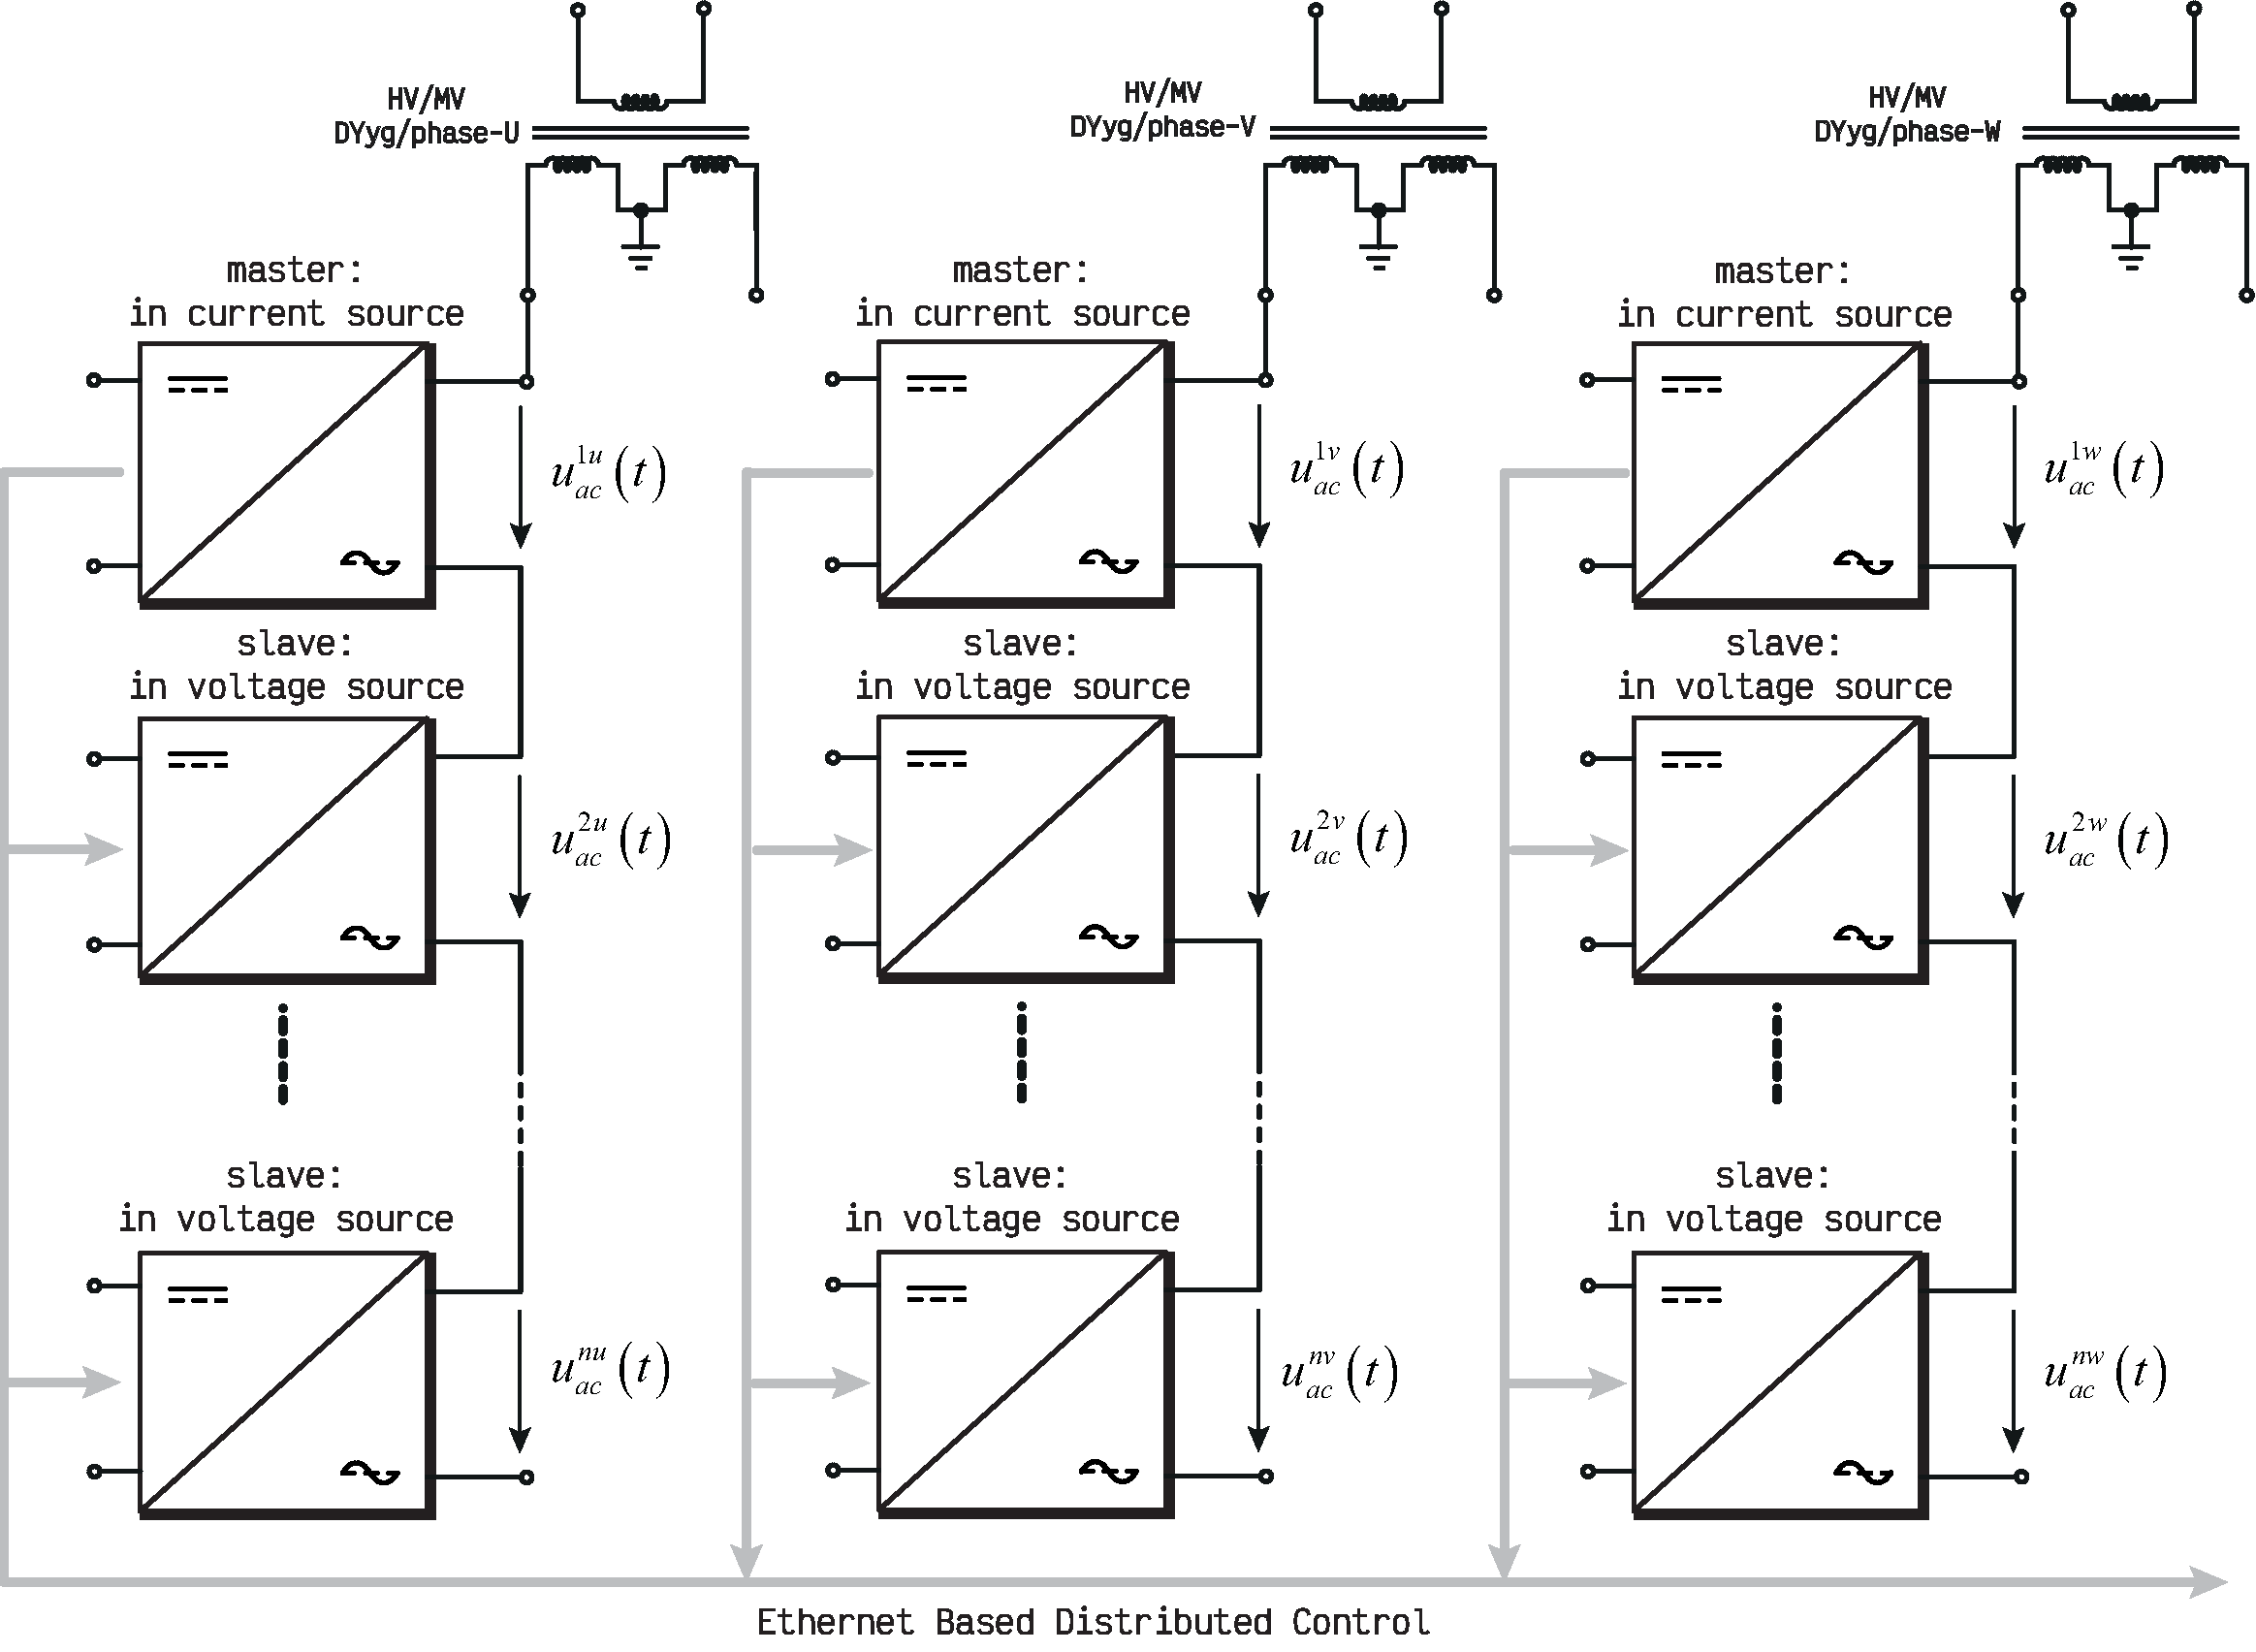
\includegraphics[width = 500pt, angle = 0, 
	keepaspectratio]{figures/arch/sst_design_ctrl_fig4c}
	\captionsetup{width=0.5\textwidth, font=small}
	\caption{Global architecture for three phase system where a cascade of master/slaves single phase inverter implements the the single phase MV.}
	\label{sst_design_ctrl_fig4c}
\end{figure}

As already mentioned, the aim of this work is to evaluate the performance of different architecture and compare them. For this purpose, single phase inverter will be investigate both by a three levels NPC and three levels T-type as shown in Figure~\ref{sst_design_ctrl_fig1b} and Figure~\ref{single_phase_inverter_ttype}. NPC solution permits to use lower voltage rated IGBT components while T-type will result in a more efficient conversion. 

\noindent\textbf{Remark} - DC-voltage rate is assumed at $U_{dc}^{\text{nom}}\SI{800}{\volt}$.

\begin{figure}[H]
	\centering
	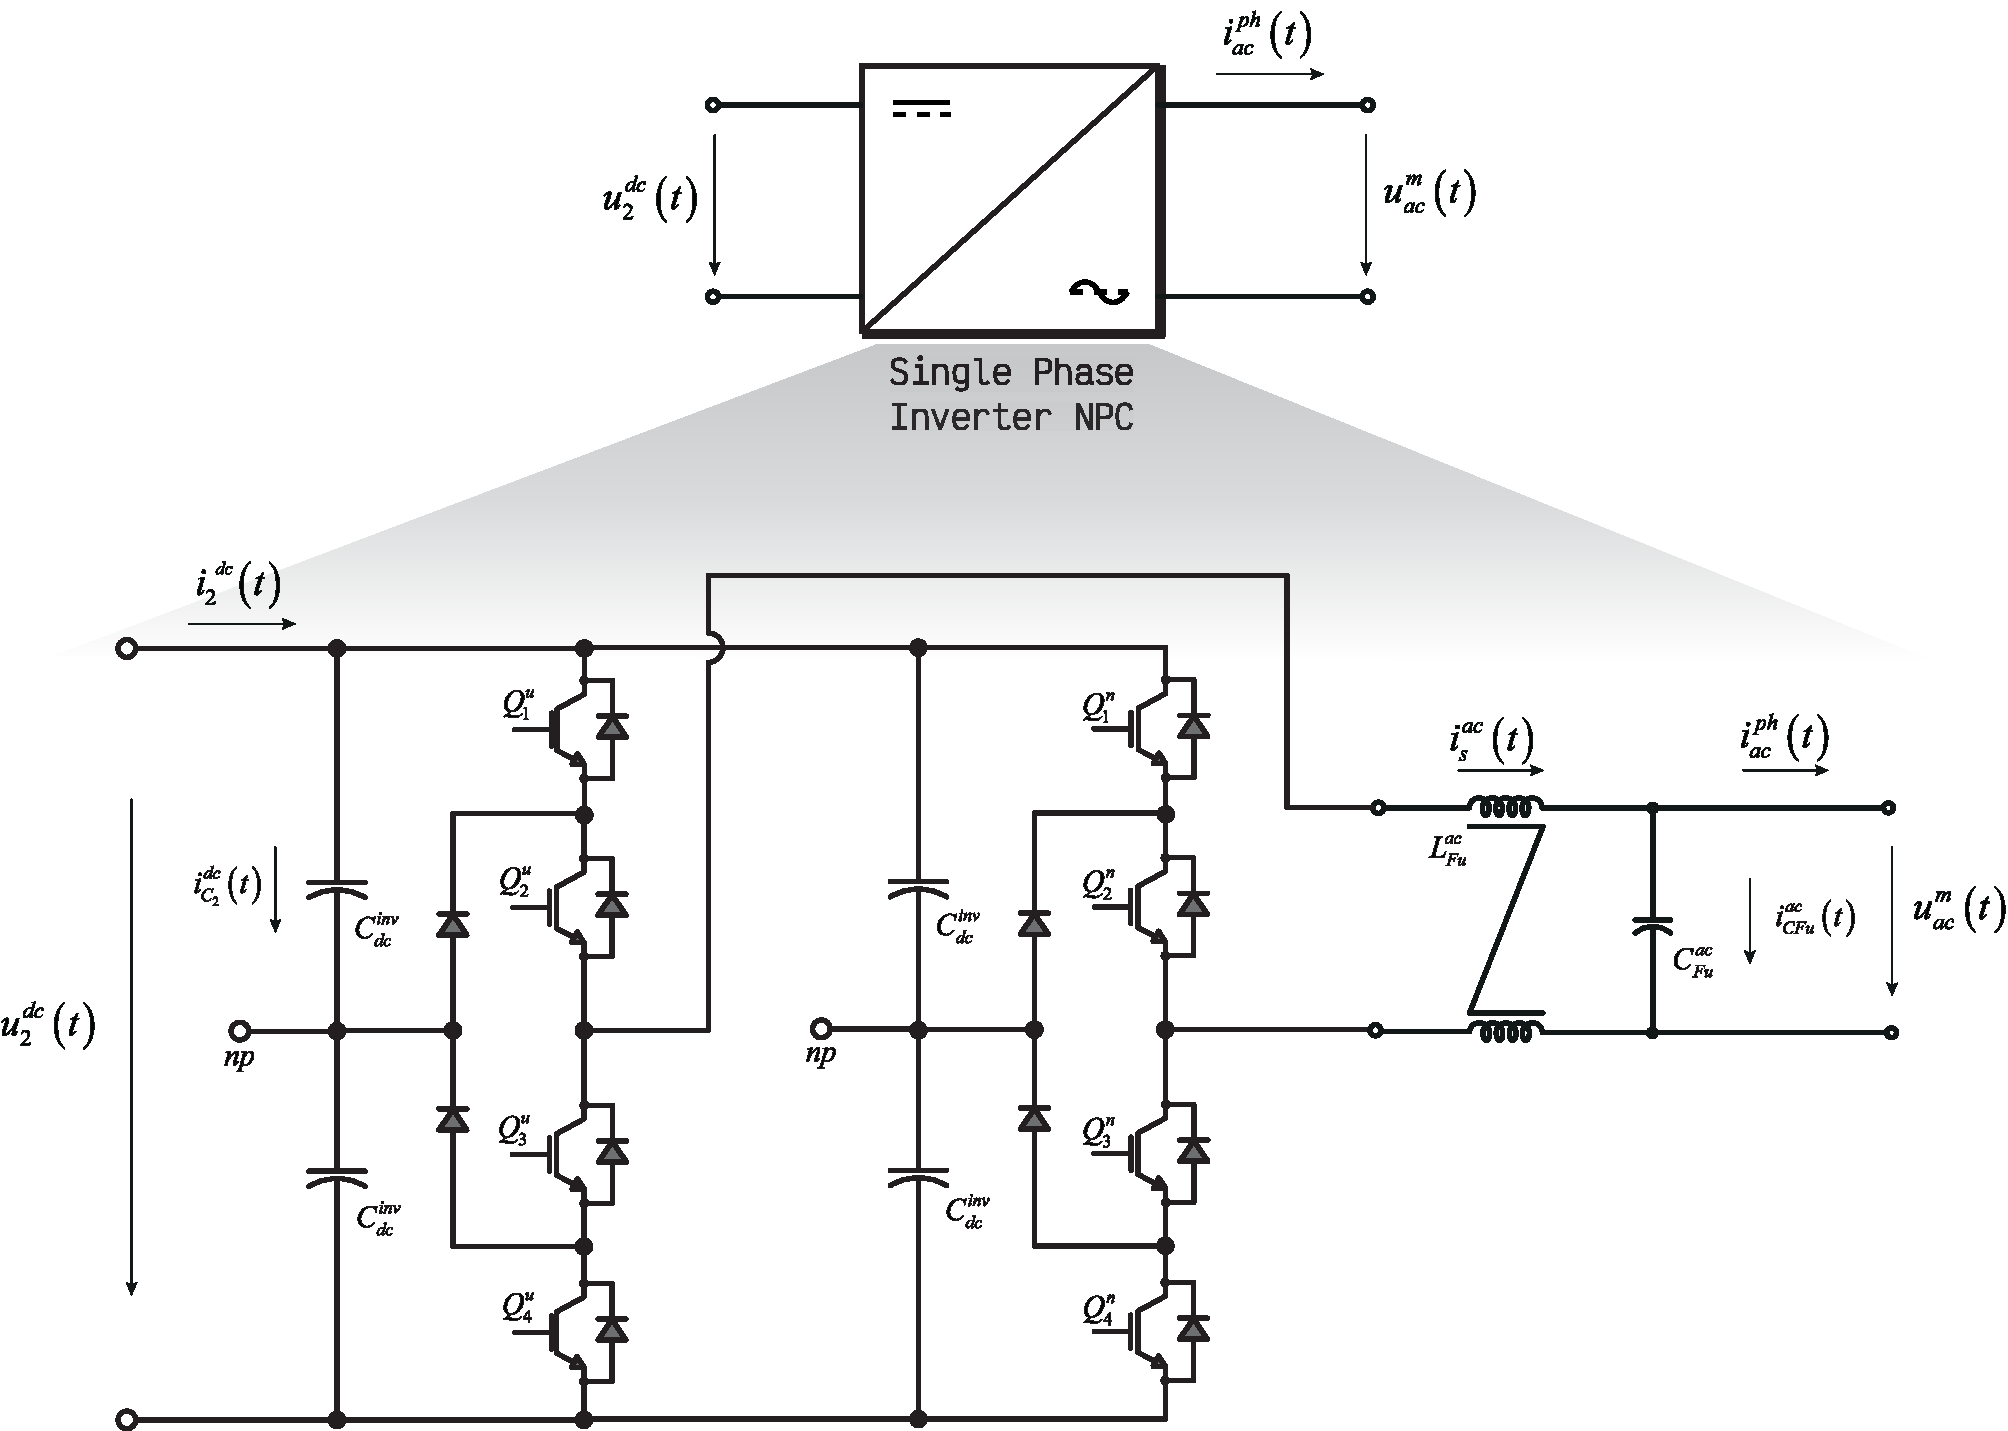
\includegraphics[width = 450pt, angle = 0, 
	keepaspectratio]{figures/arch/sst_design_ctrl_fig1b}
	\captionsetup{width=0.5\textwidth, font=small}
	\caption{Single phase inverter stage: based on three level NPC.}
	\label{sst_design_ctrl_fig1b}
\end{figure}

\begin{figure}[H]
	\centering
	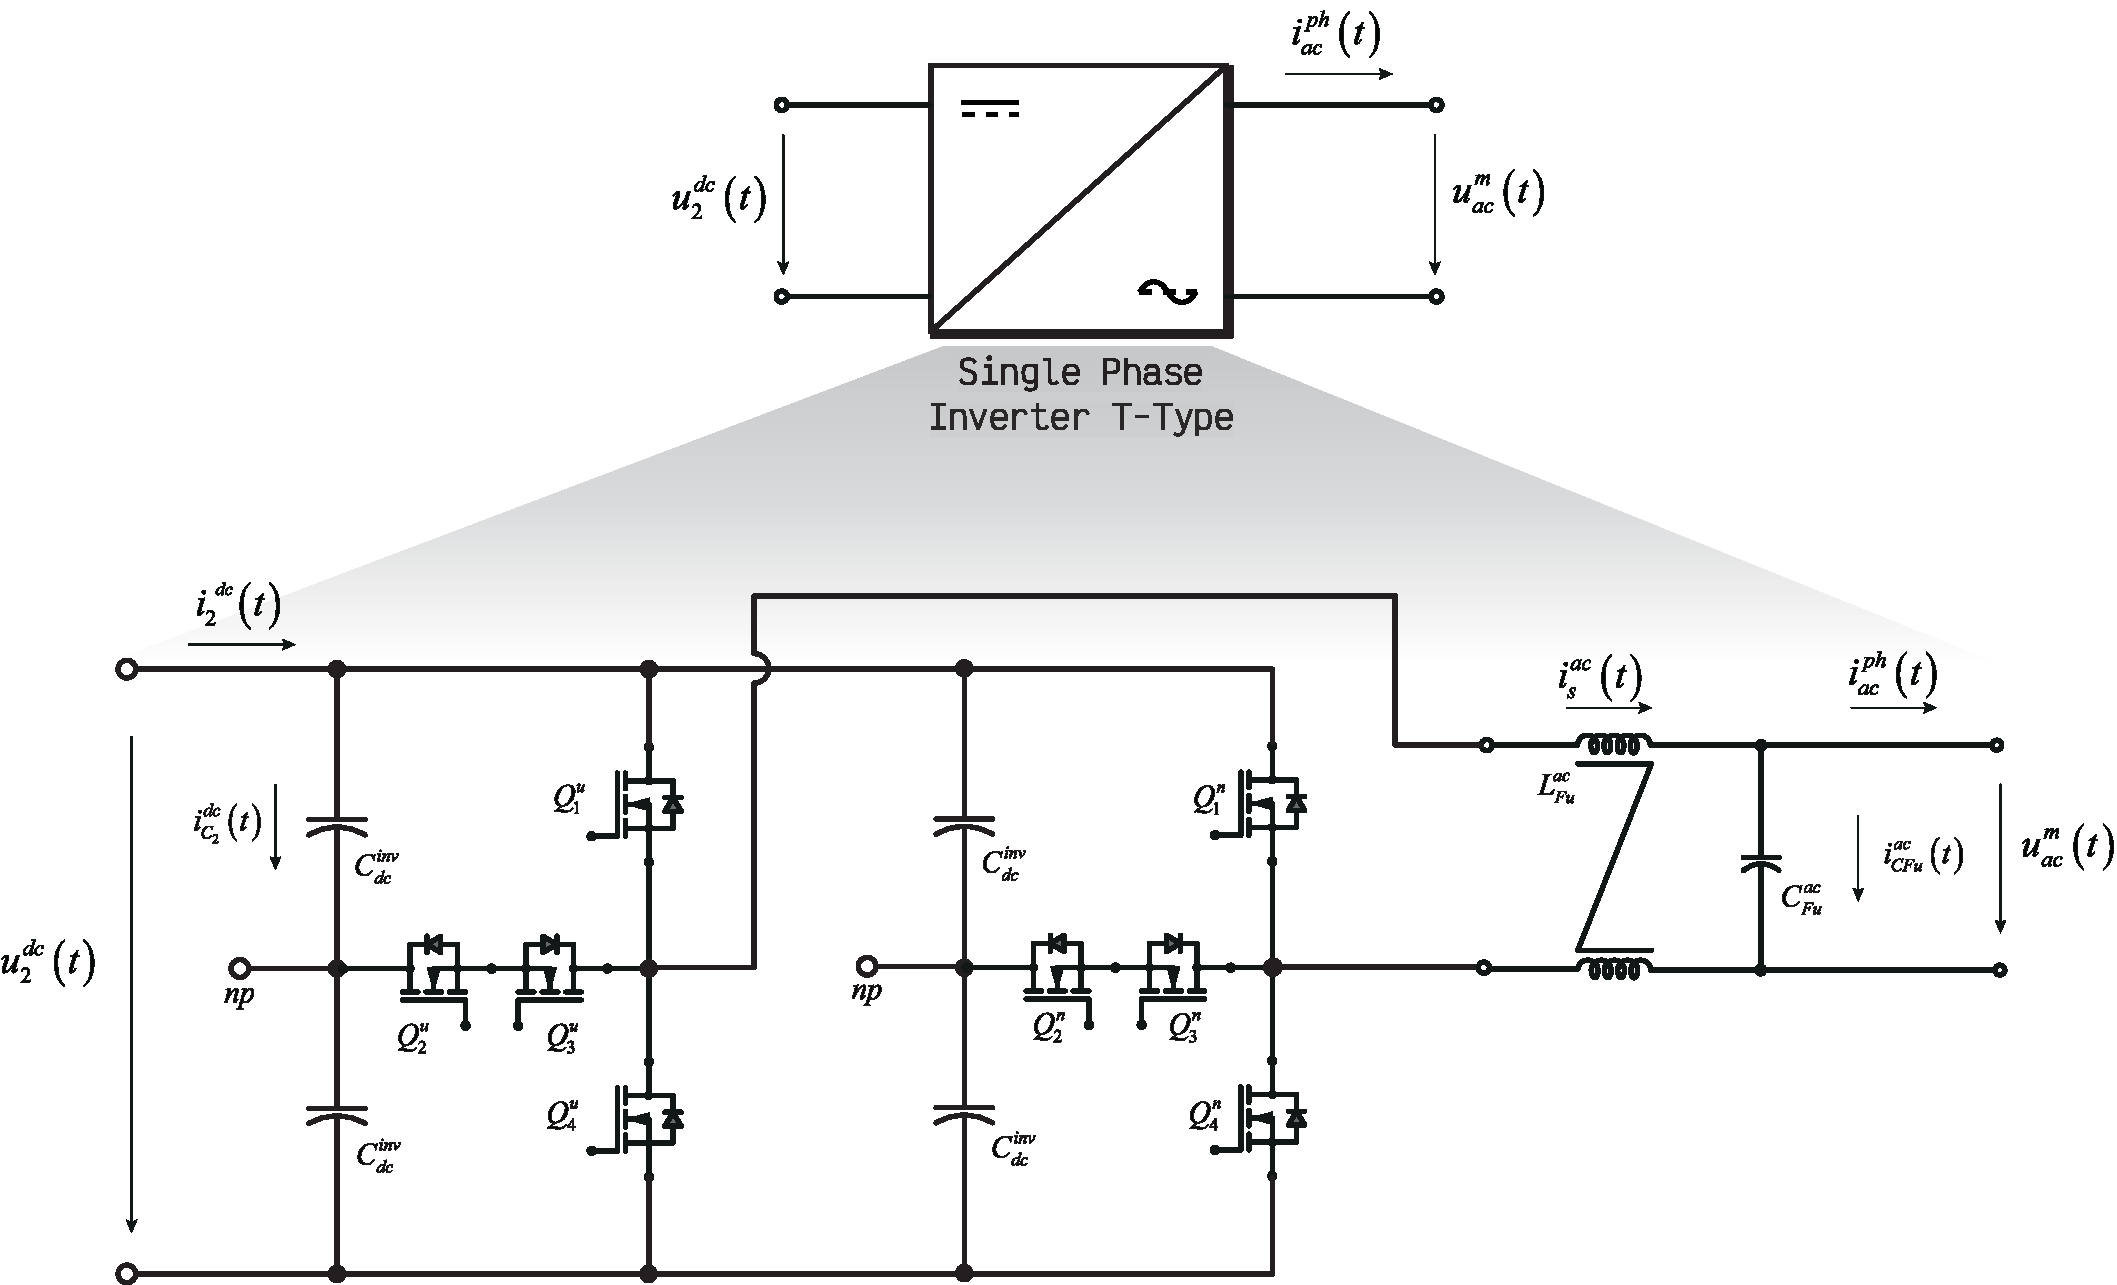
\includegraphics[width = 450pt, angle = 0, 
	keepaspectratio]{figures/arch/single_phase_inverter_ttype}
	\captionsetup{width=0.5\textwidth, font=small}
	\caption{Single phase inverter stage: based on three level T-type.}
	\label{single_phase_inverter_ttype}
\end{figure}

\noindent\textbf{Remark} - concerning the galvanically isolated DC/DC converters the following architecture will be investigated:
\begin{itemize}
	\item[--] three phase DAB;
	\item[--] single phase bidirectional CLLC;
	\item[--] single phase DAB;
\end{itemize} 

\noindent\textbf{Remark} - three phase DAB could have a better behaviour in terms of DC-current controllability, even if the topic will be more further investigated.

\begin{figure}[H]
	\centering
	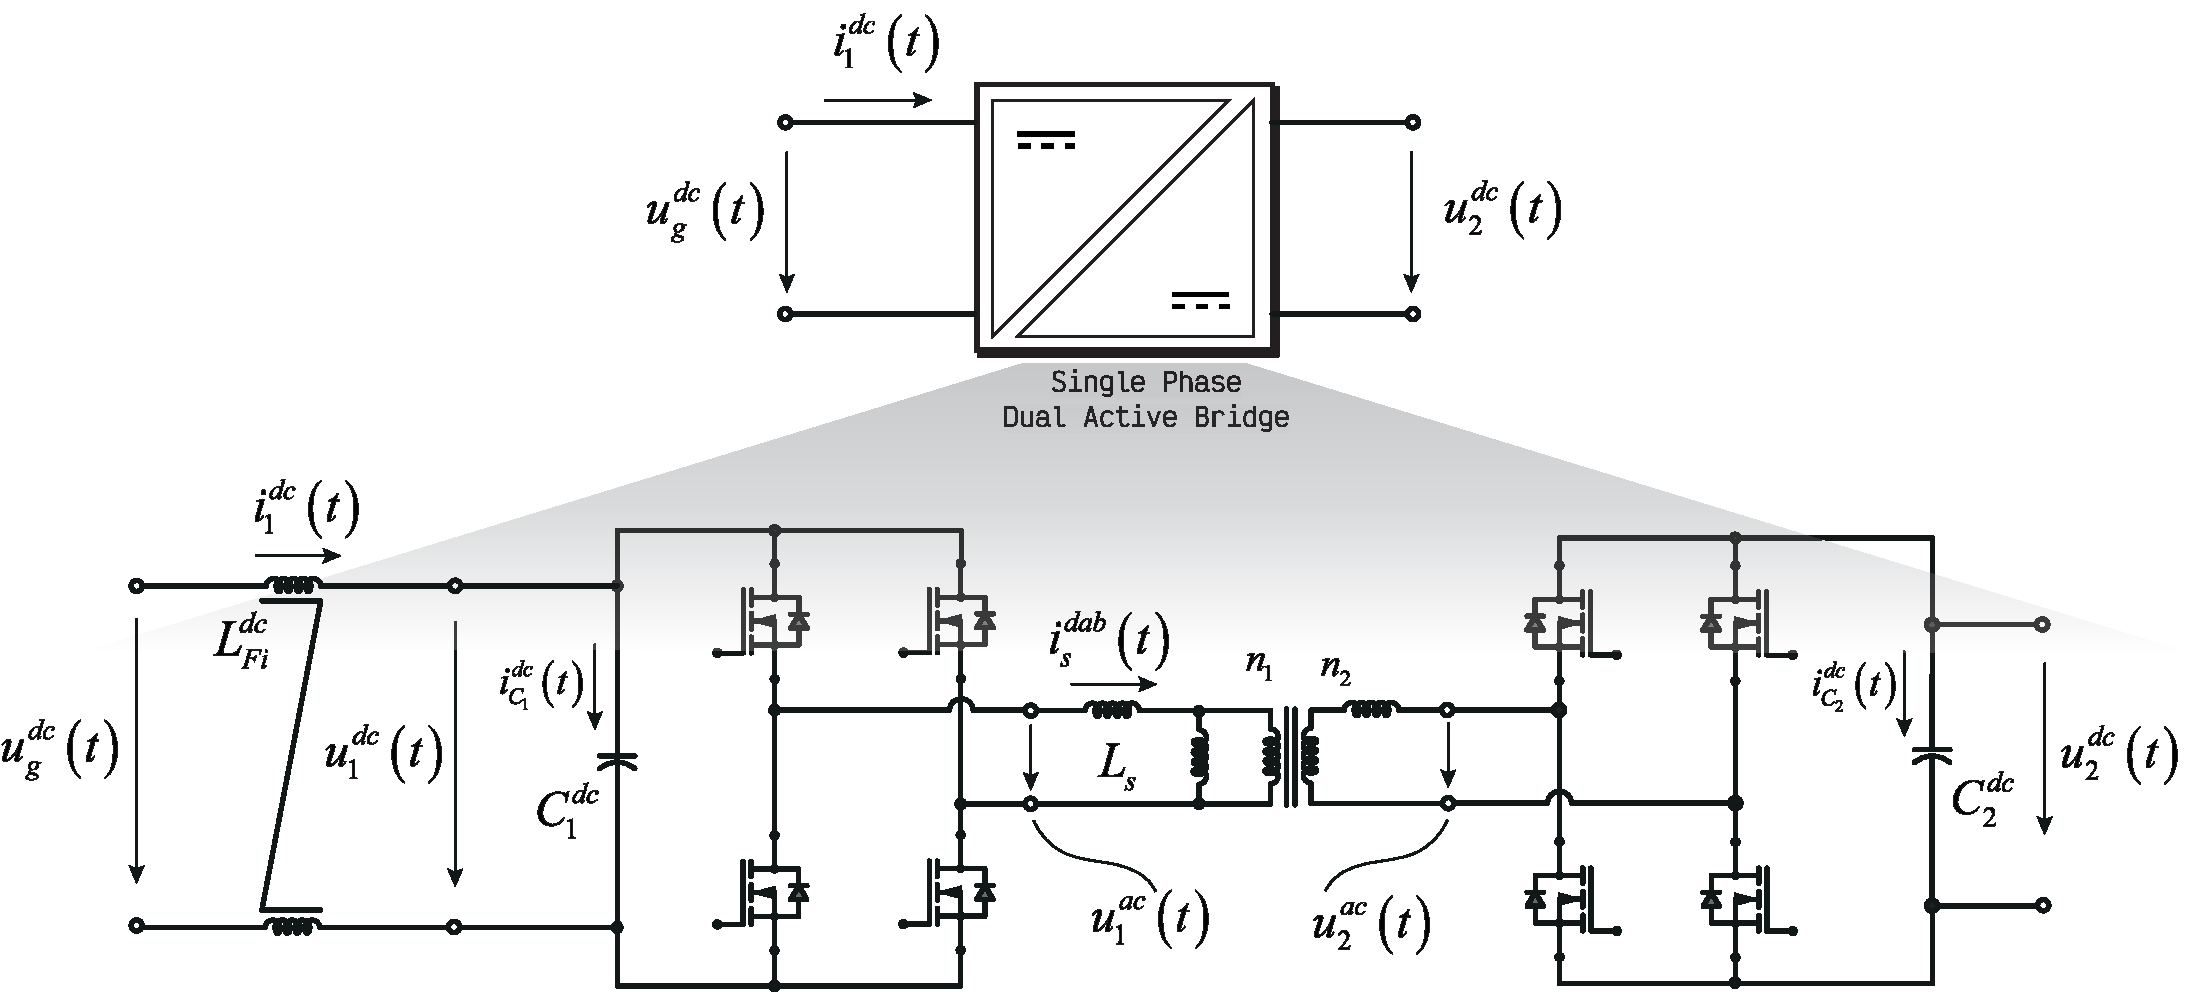
\includegraphics[width = 540pt, angle = 0, 
	keepaspectratio]{figures/arch/sst_design_ctrl_fig2}
	\captionsetup{width=0.5\textwidth, font=small}
	\caption{Single phase DAB.}
	\label{sst_design_ctrl_fig2}
\end{figure}
\begin{figure}[H]
	\centering
	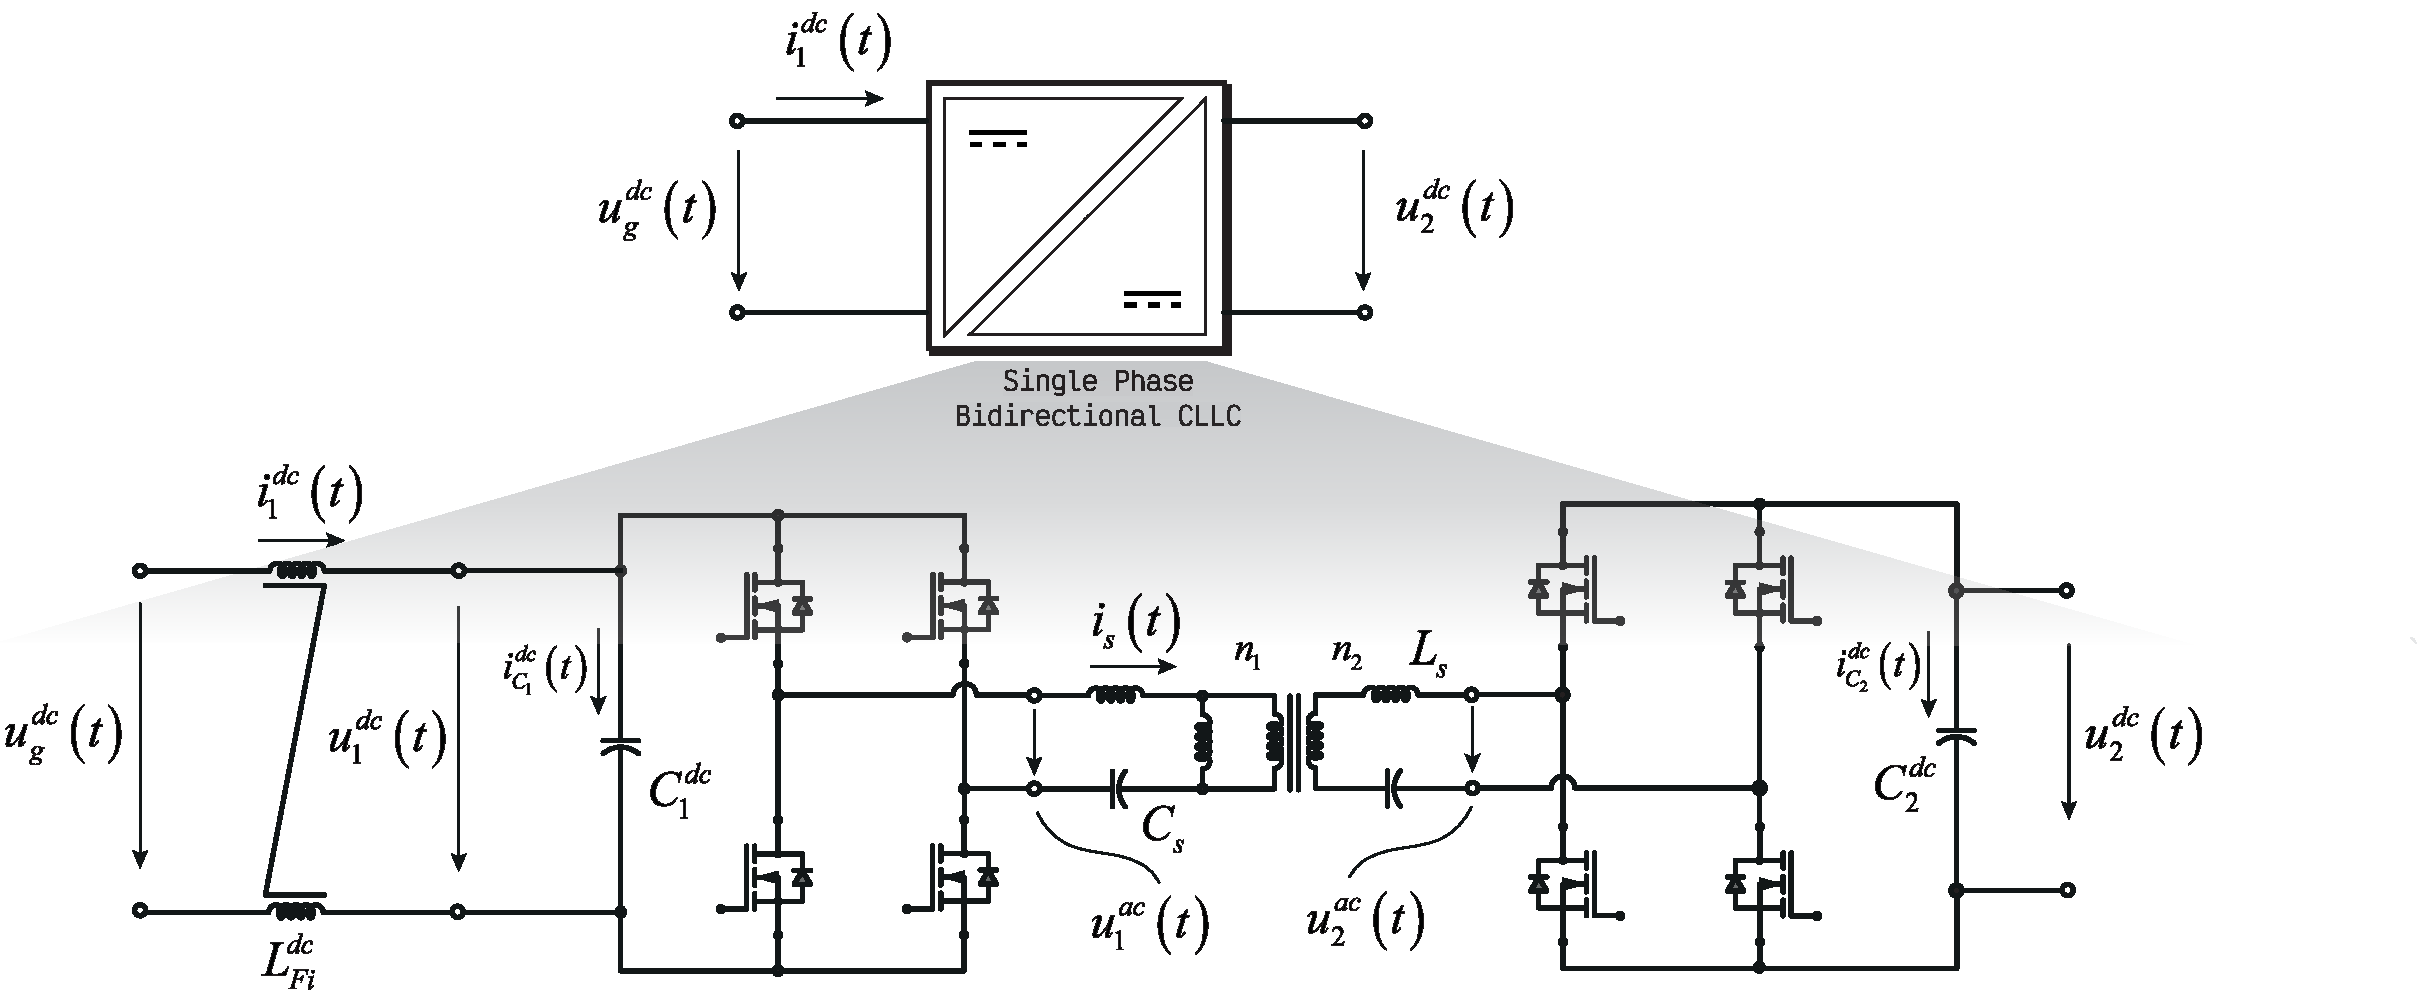
\includegraphics[width = 540pt, angle = 0, 
	keepaspectratio]{figures/arch/sst_design_ctrl_fig2c}
	\captionsetup{width=0.5\textwidth, font=small}
	\caption{Single phase bidirectional CLLC.}
	\label{sst_design_ctrl_fig2c}
\end{figure}
\begin{figure}[H]
	\centering
	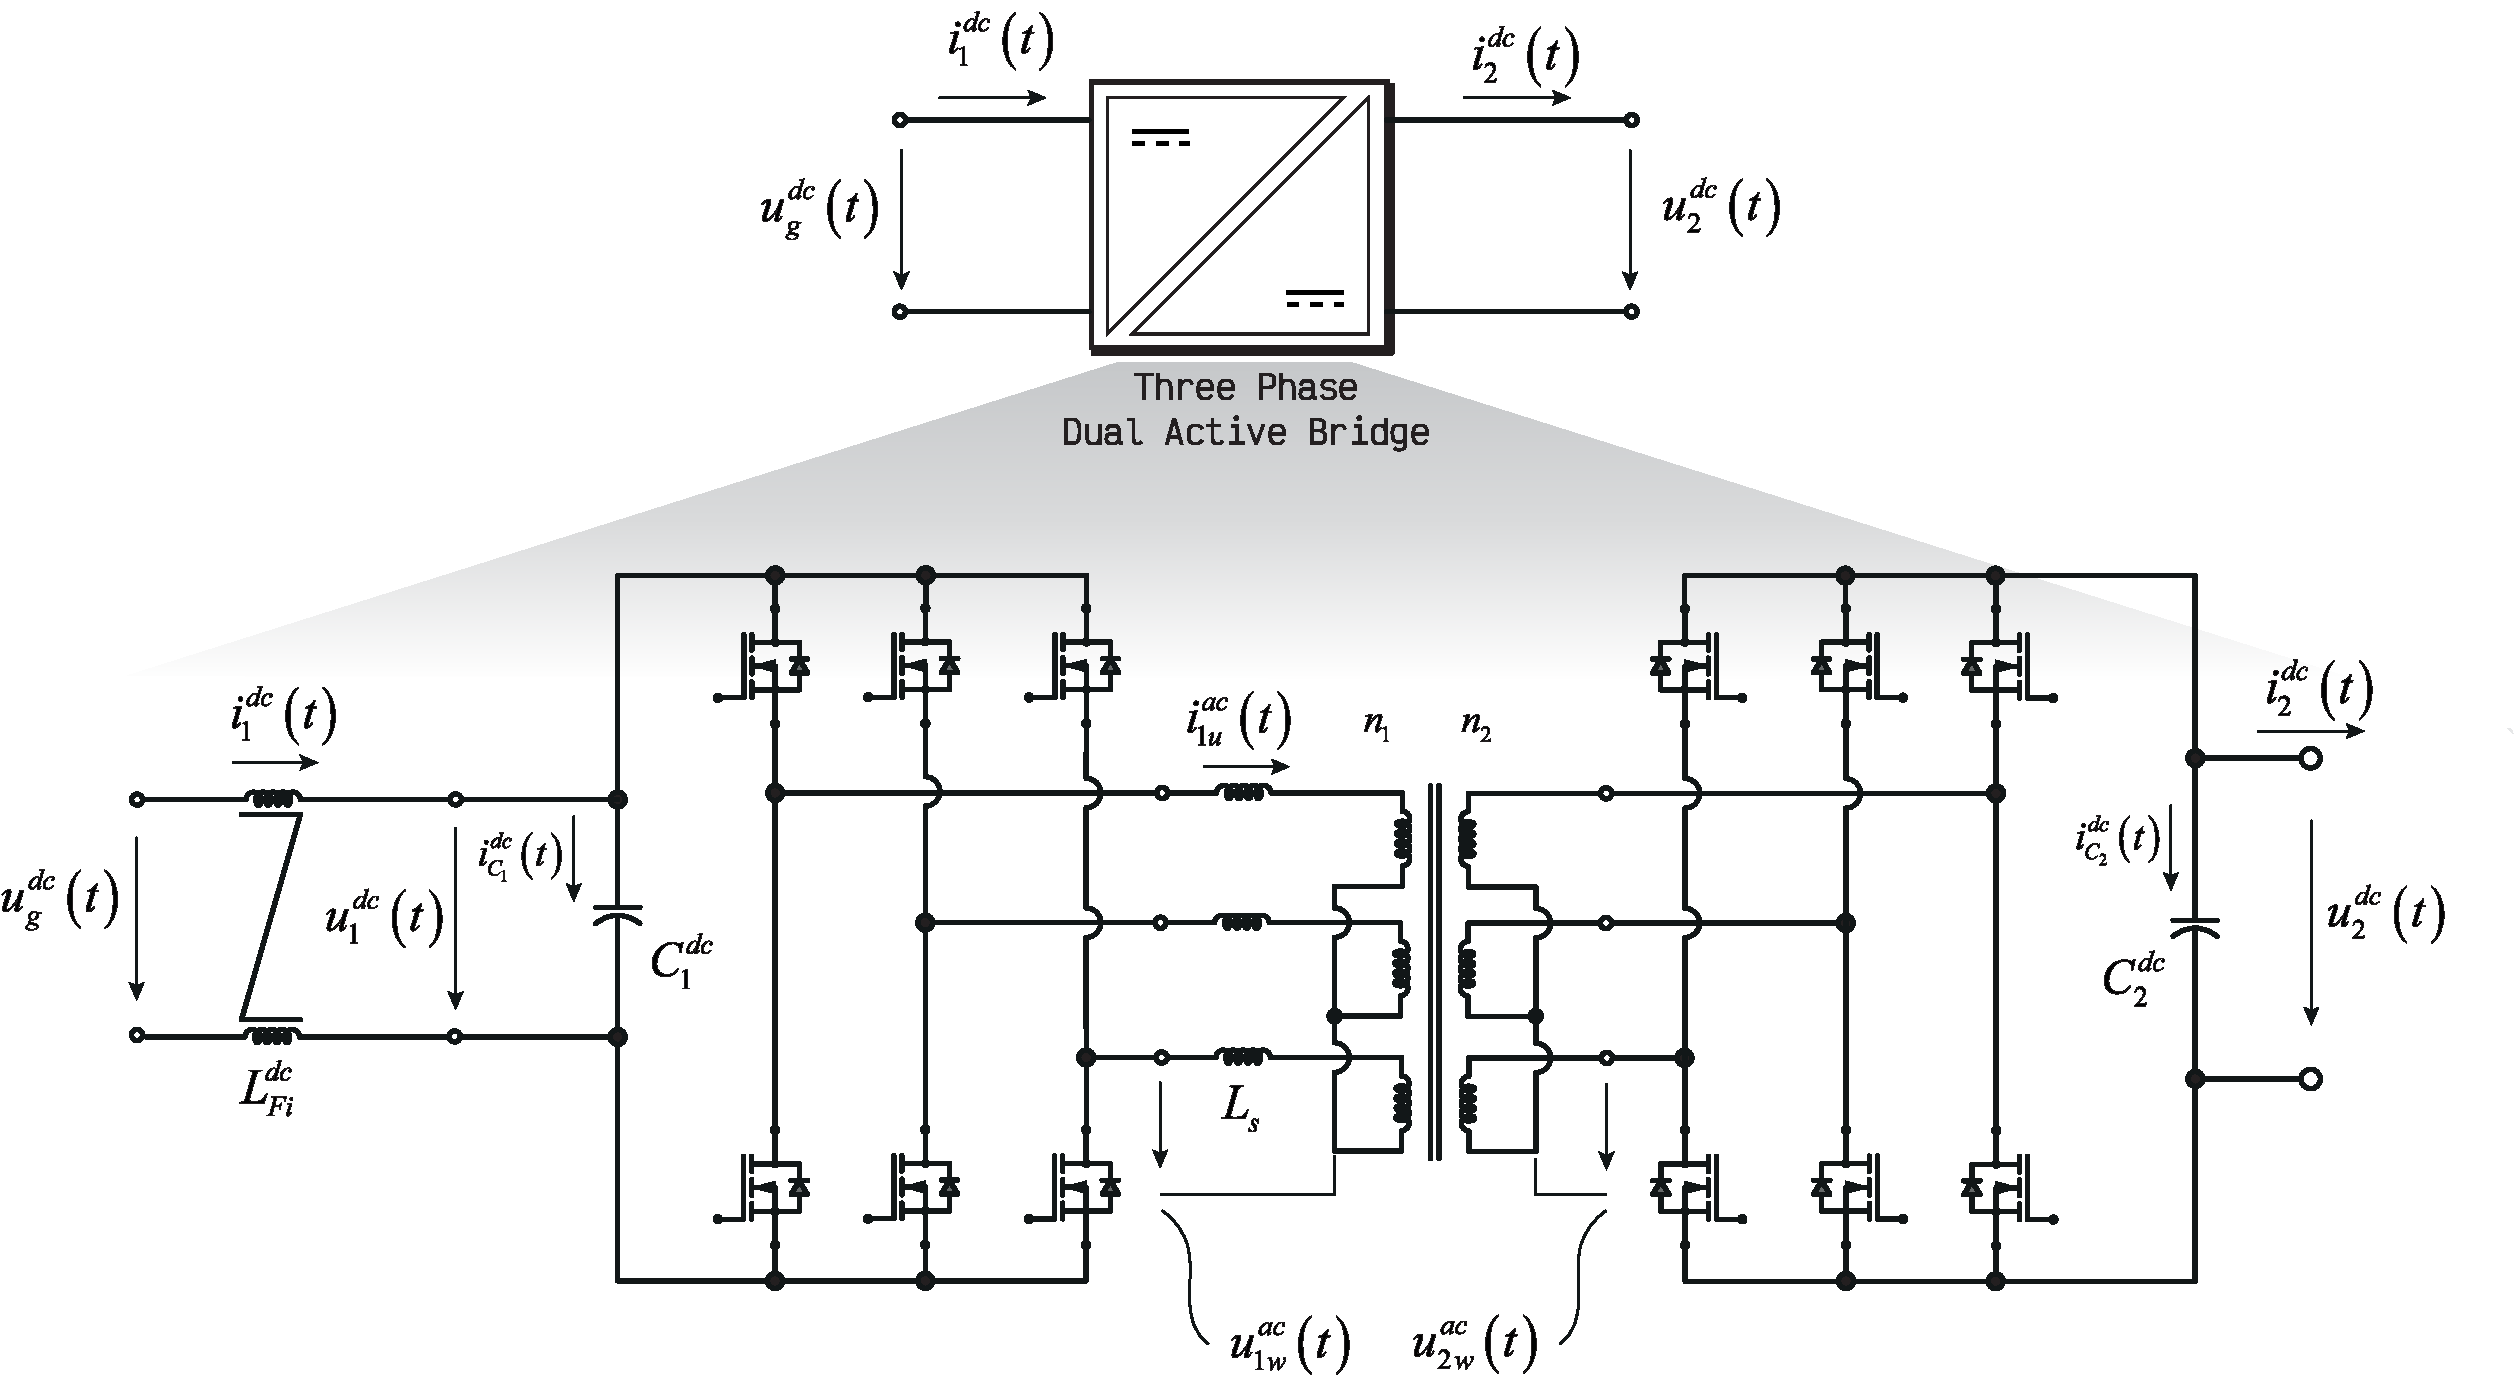
\includegraphics[width = 540pt, angle = 0, 
	keepaspectratio]{figures/arch/sst_design_ctrl_fig2b}
	\captionsetup{width=0.5\textwidth, font=small}
	\caption{Three phase DAB.}
	\label{sst_design_ctrl_fig2b}
\end{figure}






\section{Control Architecture}
\label{sec:control_arch}
The main goal for an SST architecture should be, on one side, to keep stable a DC-grid composed of many \textit{producers/consumers}, and to give an additional stability contribution to the AC-grid by properly absorbing/generating both reactive as well as active power (assuming DC-grid is integrated by energy storage systems).

Diving into the inner SST control architecture, it is assumed that each DC/DC converter provides a controlled (stable at a given value) DClink voltage, $u_2^{dc}(t) = u_2^{dc}\Big|_{ref}$, while the single phase inverter will drive a current to the AC-grid according to an outer control level\footnote{The outer control loop here intended concerns a global strategy which unified the stability of the DC-grid as well as the stability of the AC-grid according to, e.g. an optimal control based strategy.}, as shown in Figure~\ref{sst_design_ctrl_fig3} shows a possible control principle.
\begin{figure}[H]
	\centering
	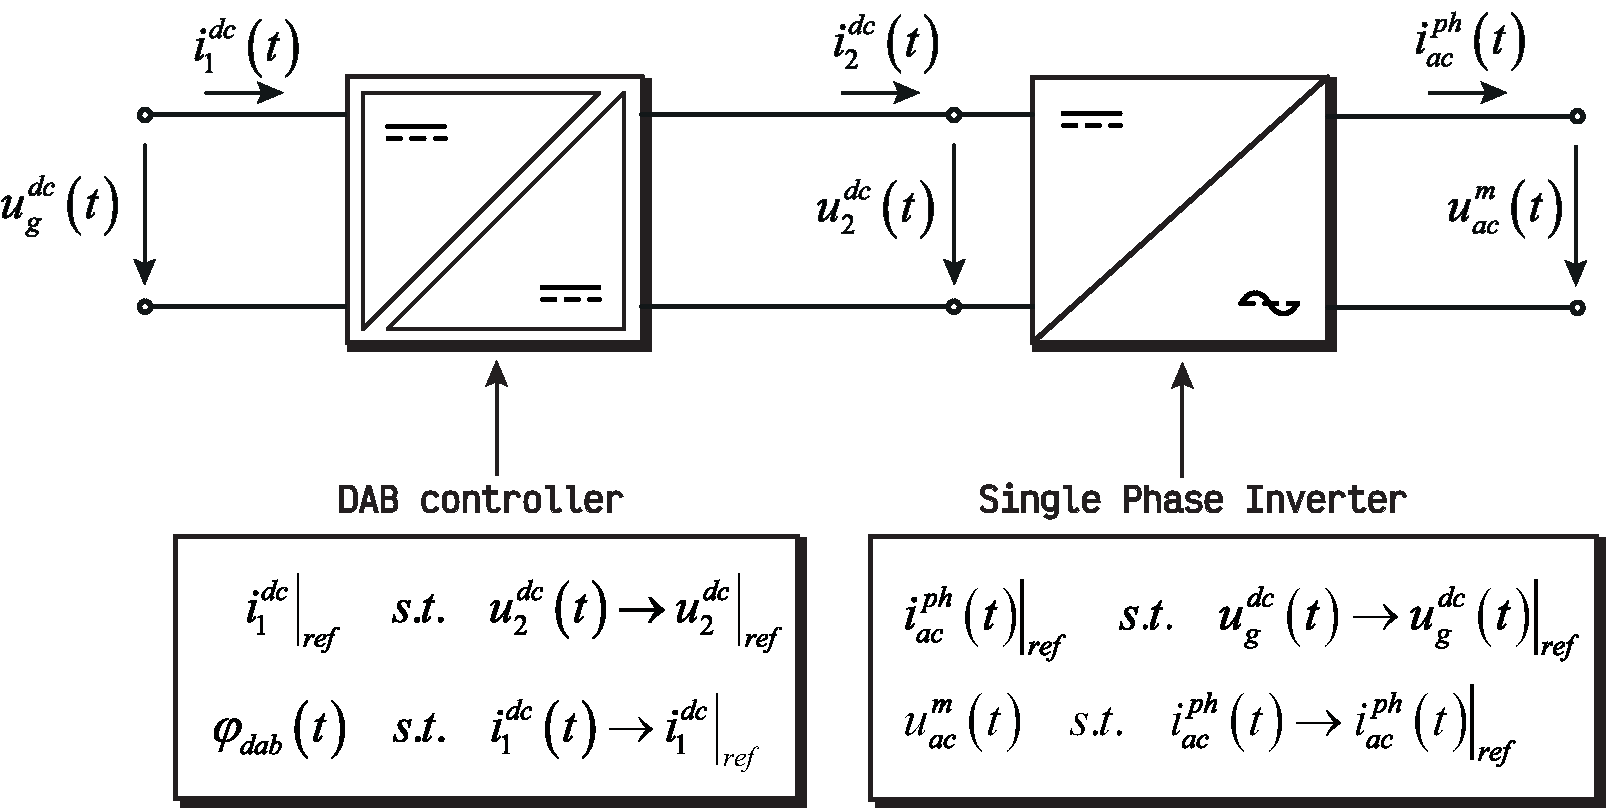
\includegraphics[width = 425pt, angle = 0, 
	keepaspectratio]{figures/arch/sst_design_ctrl_fig3}
	\captionsetup{width=0.5\textwidth, font=small}
	\caption{Fundamental control strategies of the isolated single phase inverter.}
	\label{sst_design_ctrl_fig3}
\end{figure}

\subsection{DC/DC Control Loops}
For the DAB stages (three phase and single phase) the DC/DC control is a cascade of PI controllers: an outer voltage loop on the isolated DC link $u_2^{dc}$ followed by an inner current loop, whose output is the phase displacement between the two bridges.

\noindent\textbf{Remark} - ZVS condition, for the single phase DAB, is achieved with a dead-time of $t_{dt} = \SI{400}{\nano\second}$.

\noindent\textbf{Remark} - the CLLC stage is not regulated. It runs as a DC transformer (DCX): both bridges at \SI{50}{\percent} duty, switching frequency a little below the series resonance, rectifying bridge driven as a synchronous rectifier by the sign of its own current, so that the rectifier turns off at zero current and the driving bridge commutates the magnetizing current only (ZVS). The isolated DC link follows the input bus through the turns ratio and the power is set by the inverter. The reason is quantitative: close to resonance the series reactance of the tank is small, the nominal power corresponds to a phase displacement of a few degrees, less than the dead time, and a regulated phase would force the rectifier to switch with current; the CLLC runs of Section~\ref{sec:sim_cllc} were made in this way (at \SI{13}{\kilo\hertz}, with the rectifier in discontinuous conduction) and the \SI{50}{\kilo\hertz} stage of the 2026 bench is designed on the same principle, see \cite{cllc_dcx_doc}.

\subsection{Single Phase Lock Loop}
Single phase inverter uses a single phase lock loop as shown in Figure~\ref{single_phase_pll_fig1}

\begin{figure}[H]
	\centering
	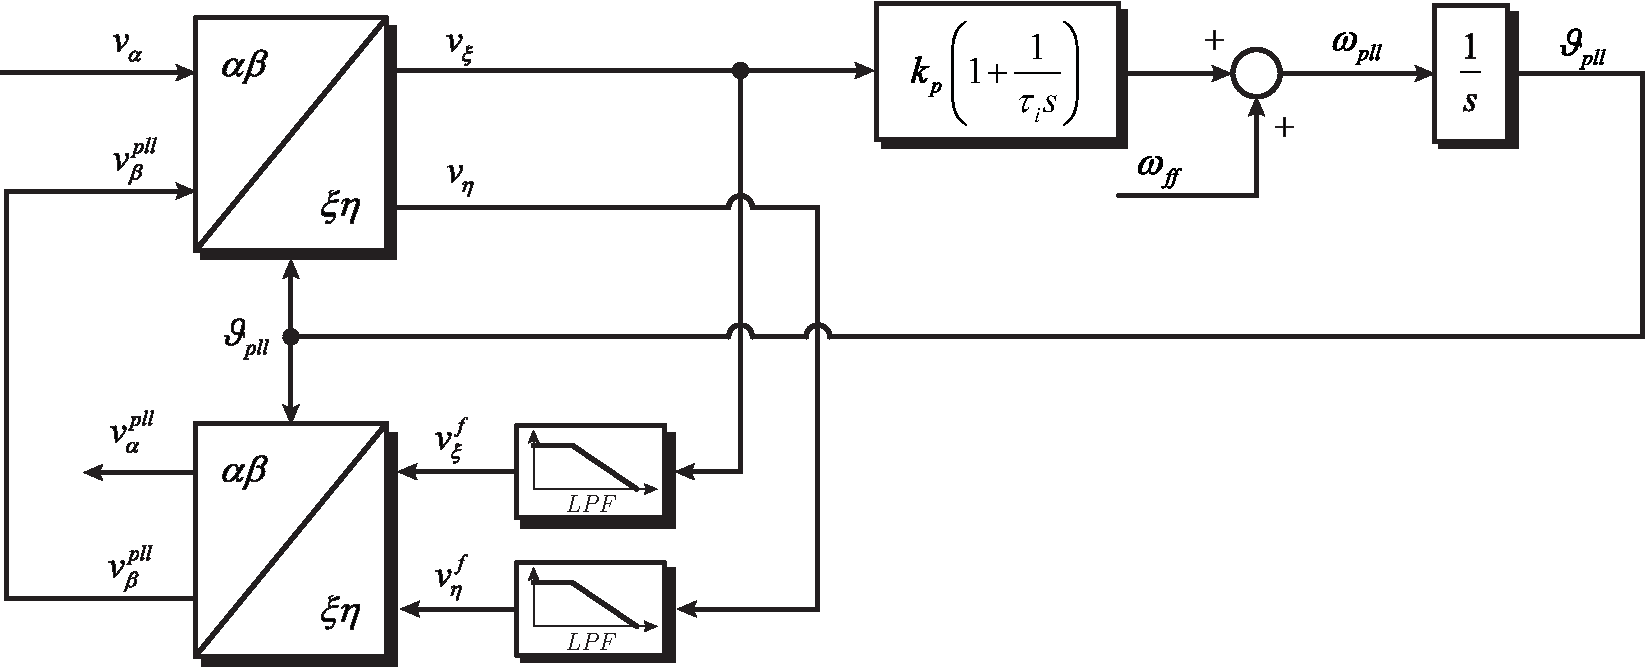
\includegraphics[width = 425pt, angle = 0, 
	keepaspectratio]{figures/control/single_phase_pll_fig1}
	\captionsetup{width=0.5\textwidth, font=small}
	\caption{Single phase lock loop for grid phase estimation.}
	\label{single_phase_pll_fig1}
\end{figure}


\subsection{Single Phase Inverter Control Layouts}
Single phase inverter has been simulated with resonant PI as well as with virtual vector control as shown in Figure~\ref{single_phase_afe_control_1}

\begin{figure}[H]
	\centering
	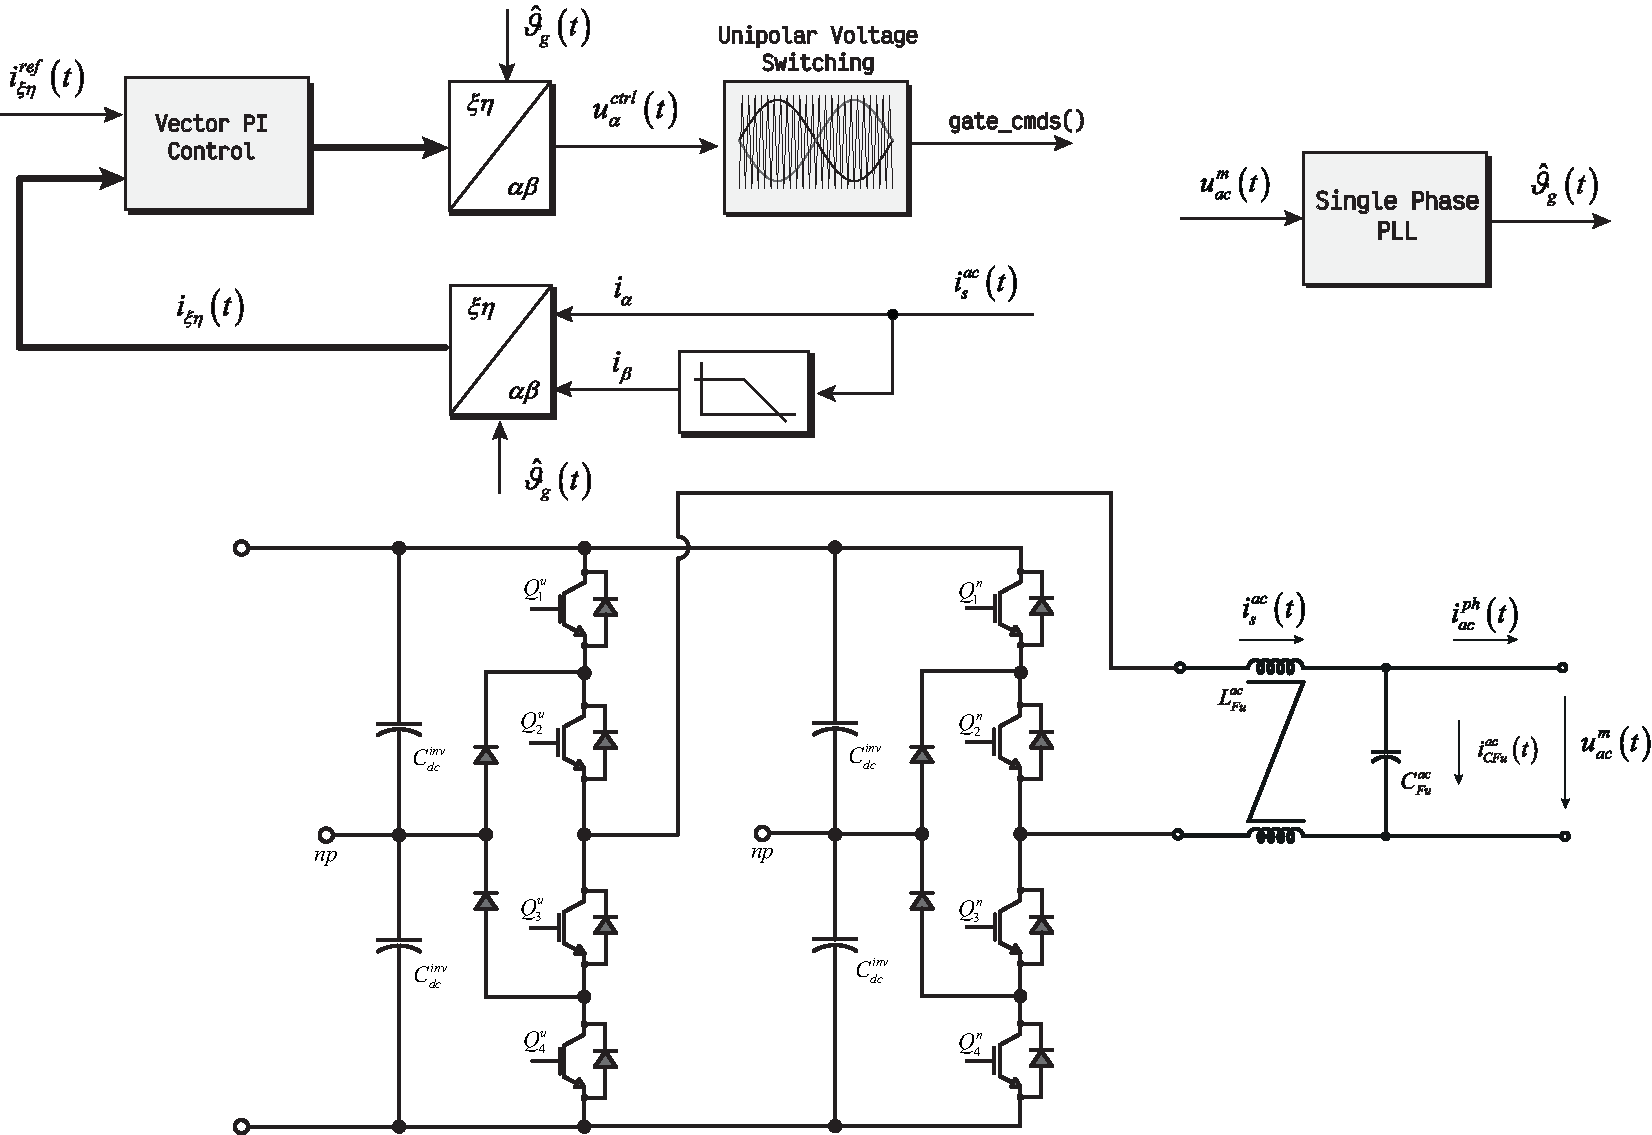
\includegraphics[width = 500pt, angle = 0, 
	keepaspectratio]{figures/control/single_phase_afe_control_1}
	\captionsetup{width=0.5\textwidth, font=small}
	\caption{Control layout of the single phase inverter. Same strategy for T-Type.}
	\label{single_phase_afe_control_1}
\end{figure}

\section{Simulation results}
\label{sec:sim_results}
\noindent\textbf{Remark (Rev.~01)} - the results of this section are those of the comparative study of 2025, at about \SI{250}{\kilo\watt} per module with the devices and the frequencies listed below. The models they were produced with are no longer in the tree of the repository; the bench that replaced them (\SI{50}{\kilo\watt} per module, CLLC-DCX at \SI{50}{\kilo\hertz} and T-type inverter) is described in Section~\ref{sec:bench2026}.

In this section simulation results of the architecture based on three phase DAB is shown, in particular the following operative conditions have been accounted:
\begin{itemize}
	\item[--] three phase DAB works at fundamental frequency of $f_{dab} = \SI{4}{\kilo\hertz}$;	
	\item[--] single phase CLLC works at fundamental frequency of $f_{llc} = \SI{13}{\kilo\hertz}$;
	\item[--] single phase DAB works at fundamental frequency of $f_{spdab} = \SI{12}{\kilo\hertz}$;
	\item[--] single phase inverter operates at the switching frequency of  $f_{inv}^{pwm} = \SI{4}{\kilo\hertz}$, both NPC and T-Type.
\end{itemize}

\noindent\textbf{Remark} - the following switching devices have been used selected
\begin{itemize}
	\item[--] Wolfspeed \textbf{CAB450M12XM3} for the three phase DAB;
	\item[--] Wolfspeed \textbf{CAB760M12HM3} for the single phase DAB and CLLC;
	\item[--] Wolfspeed \textbf{CAB760M12HM3} for the NPC (the number of paralleled device is two);
	\item[--] Wolfspeed \textbf{CAB760M12HM3} + \textbf{CLB800M12HM3P} for the T-Type (the number of paralleled device is two);
\end{itemize}

According to Figure~\ref{sst_design_ctrl_fig2c} and Figure~\ref{sst_design_ctrl_fig1b}, the following components shall be accounted:
\begin{itemize}
	\item[--] $L_{Fi}^{dc} = \SI{400}{\micro\henry}$ - input DAB inductance with nominal current of $I_{LFu}^{nom} = \SI{325}{\ampere}$;
	\item[--] $C_{1}^{dc} = \SI{3.6}{\milli\farad}$ - input DAB capacitor with nominal voltage of $U_{dc1}^{nom} = \SI{800}{\volt}$;
	\item[--] $C_{2}^{dc} = \SI{3.6}{\milli\farad}$ - output DAB capacitor with nominal voltage of $U_{dc2}^{nom} = \SI{800}{\volt}$;
	\item[--] $C_{dc}^{inv} = \SI{3.6}{\milli\farad}$ - single phase DClink capacitor, with nominal voltage of $U_{dc}^{nom} = \SI{400}{\volt}$;
	\item[--] $L_{Fu}^{ac} = \SI{300}{\micro\henry}$ - output single phase inverter inductance with nominal current $I_{LFu}^{nom} = \SI{1000}{\ampere}$;
	\item[--] $C_{Fu}^{ac} = \SI{360}{\micro\henry}$ - output single phase inverter capacitor with nominal voltage of $U_{CFu}^{nom} = \SI{270}{\volt}$;
	\item[--] $L_s = \SI{28}{\micro\henry}$ - three phase DAB inductance (this value takes into account also the leakage inductance of the transformer) with nominal current of $I_{Ls}^{nom} = \SI{250}{\ampere}$ at nominal frequency of $f_{Ls}^{nom} = \SI{4}{\kilo\hertz}$;
	\item[--] $L_s = \SI{11}{\micro\henry}$ - single phase DAB inductance (this value takes into account also the leakage inductance of the transformer) with nominal current of $I_{Ls}^{nom} = \SI{400}{\ampere}$ at nominal frequency of $f_{Ls}^{nom} = \SI{12}{\kilo\hertz}$;
	\item[--] $L_s = \SI{13}{\micro\henry}$ - single phase CLLC inductance (this value takes into account also the leakage inductance of the transformer) with nominal current of $I_{Ls}^{nom} = \SI{450}{\ampere}$ at nominal frequency of $f_{Ls}^{nom} = \SI{13}{\kilo\hertz}$;
	\item[--] $C_{s1} = C_{s2} = \SI{10}{\micro\farad}$ - single phase CLLC resonant capacitor ($f_{res} = \SI{20}{\kilo\hertz}$) with nominal current of $I_{Cs}^{nom} = \SI{450}{\ampere}$;
\end{itemize}
Figure~\ref{single_phase_afe_control_1} show the control architecture of the single phase inverter.
\begin{figure}[H]
	\centering
	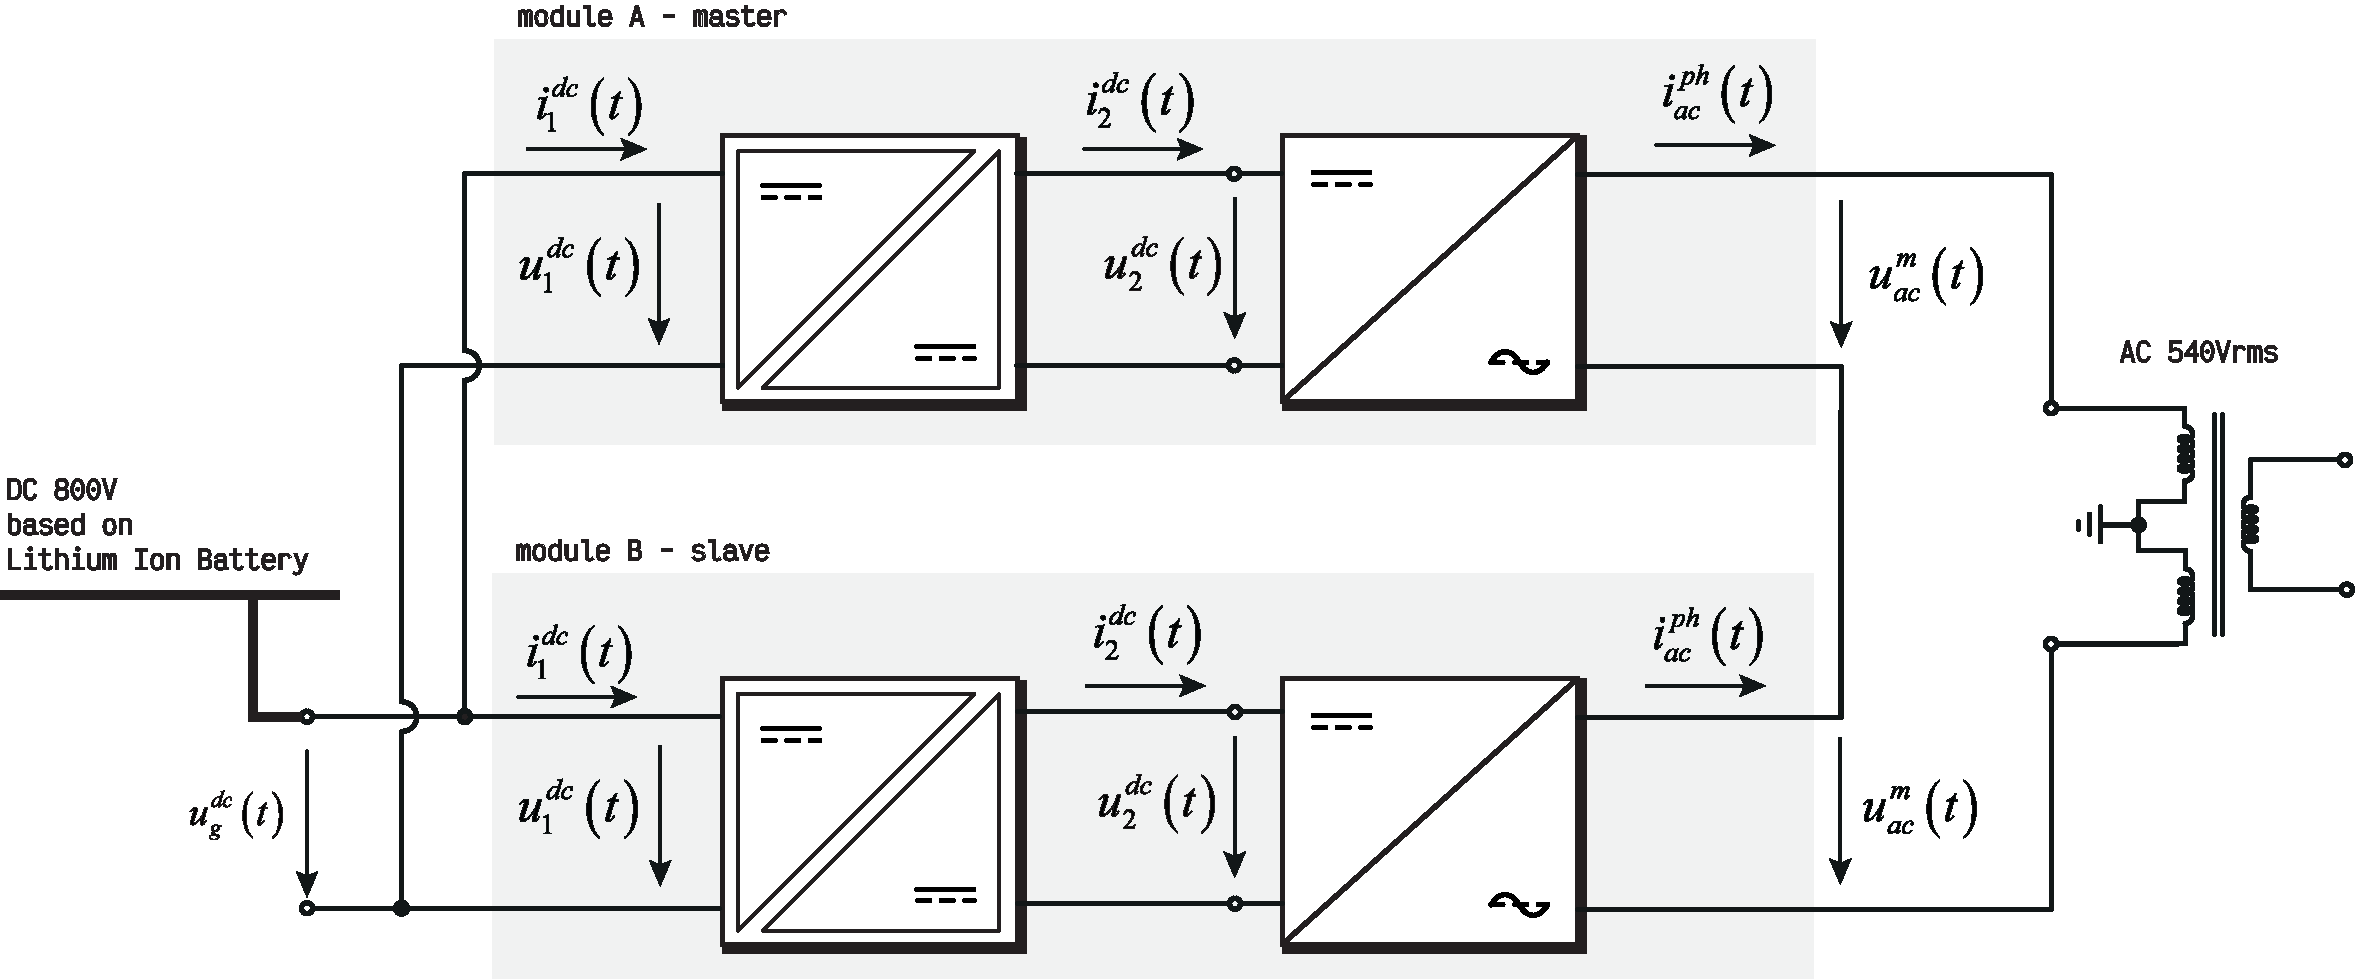
\includegraphics[width = 500pt, angle = 0, 
	keepaspectratio]{figures/sim_results/simulation_layout}
	\captionsetup{width=0.75\textwidth, font=small}
	\caption{Simulation layout: simulation has been performance using a single phase SST composed by two single phase inverter connected in series with three difference case scenario of DCDC: three phase DAB, single phase DAB, and single phase CLLC.}
	\label{simulation_layout}
\end{figure}


\subsection{SST based on Three Phase DAB and NPC Single Phase Inverter}
Here performance of the SST based on three phase DAB and a cascade of two three level NPC/T-Type single phase inverters.

\noindent\textbf{Remark} - only one single phase has been simulated and the total power at DC grid side is resulting in one third of an equivalent three phase implementation.

\noindent\textbf{Remark} - simulations have been performed under the following condition of grids and load:
\begin{itemize}
	\item[--] DC grid nominal voltage (from Lithium Ion Battery) : $u_{g}^{dc}\Big|_{nom} = \SI{750}{\volt}-\SI{800}{\volt}$;
	\item[--] AC grid nominal voltage : $u_{g}^{ac}\Big|_{nom} = \SI{540}{\volt}$ - rms per phase-centertap;
	\item[--] AC grid load current : $i_{g}^{ac} = \SI{1000}{\ampere}$ - rms;
\end{itemize}

\begin{figure}[H]
	\centering
	\begin{subfigure}{0.5\textwidth}
		\centering
		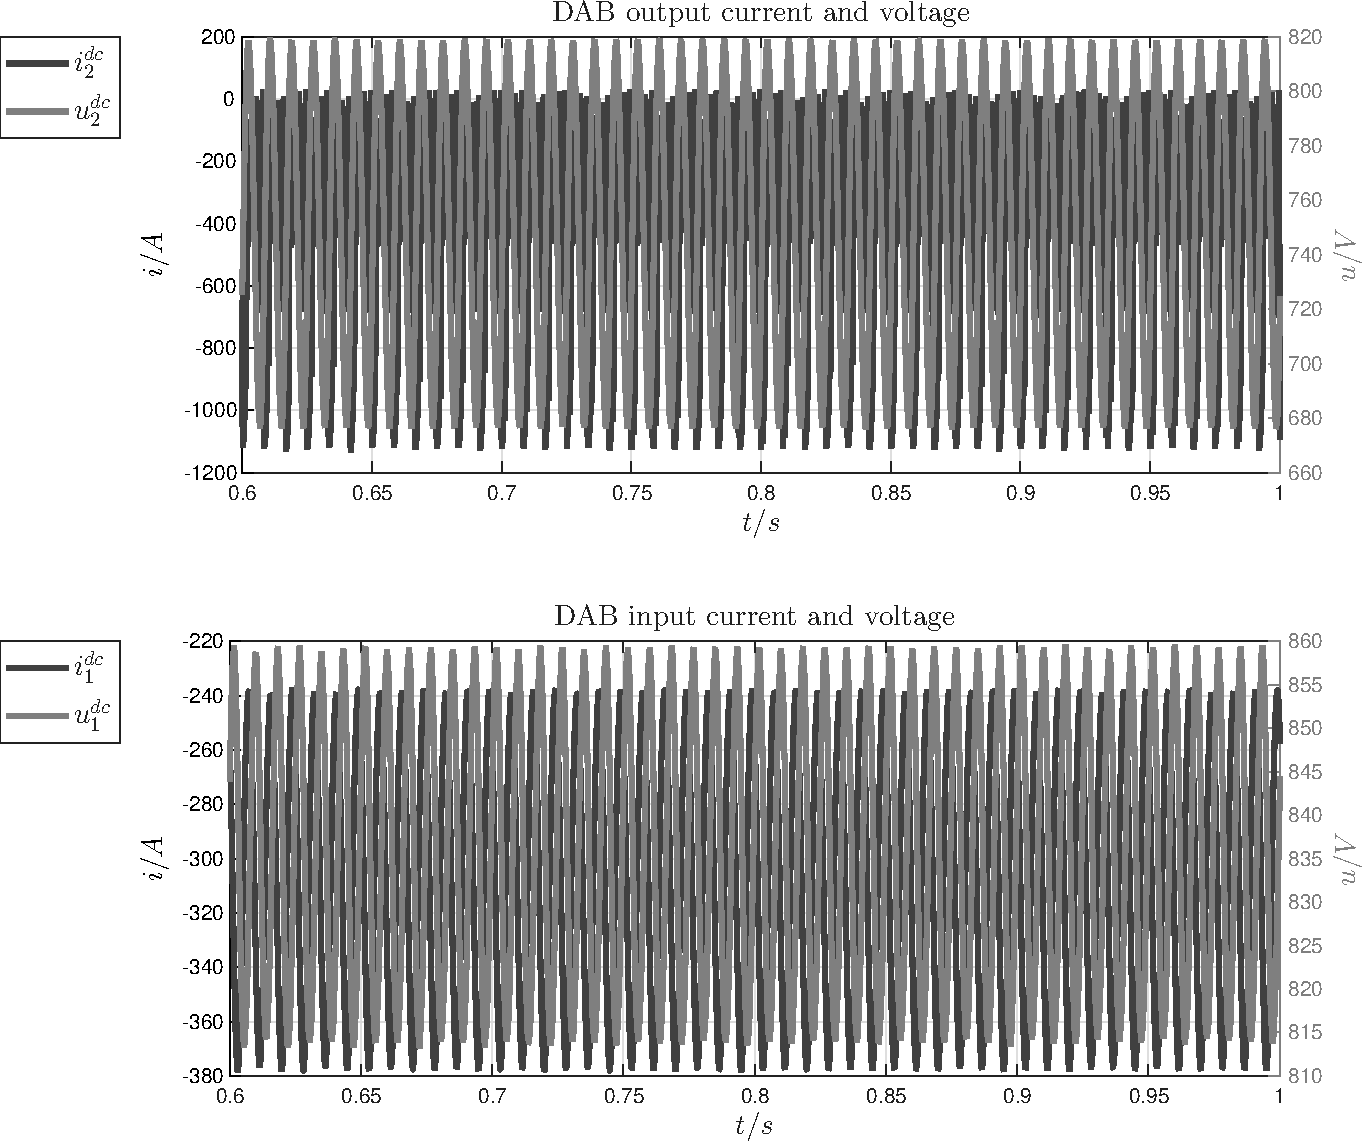
\includegraphics[width =225pt, angle = 0, 
		keepaspectratio]{figures/sim_results/three_phase_dab/dab_ui_output_input}
		\captionsetup{width=0.95\textwidth, font=footnotesize}	
		\caption{Master three phase DAB input current and voltage (bottom) and outputs (top).}
		\label{}
	\end{subfigure}%
	\begin{subfigure}{0.5\textwidth}
		\centering
		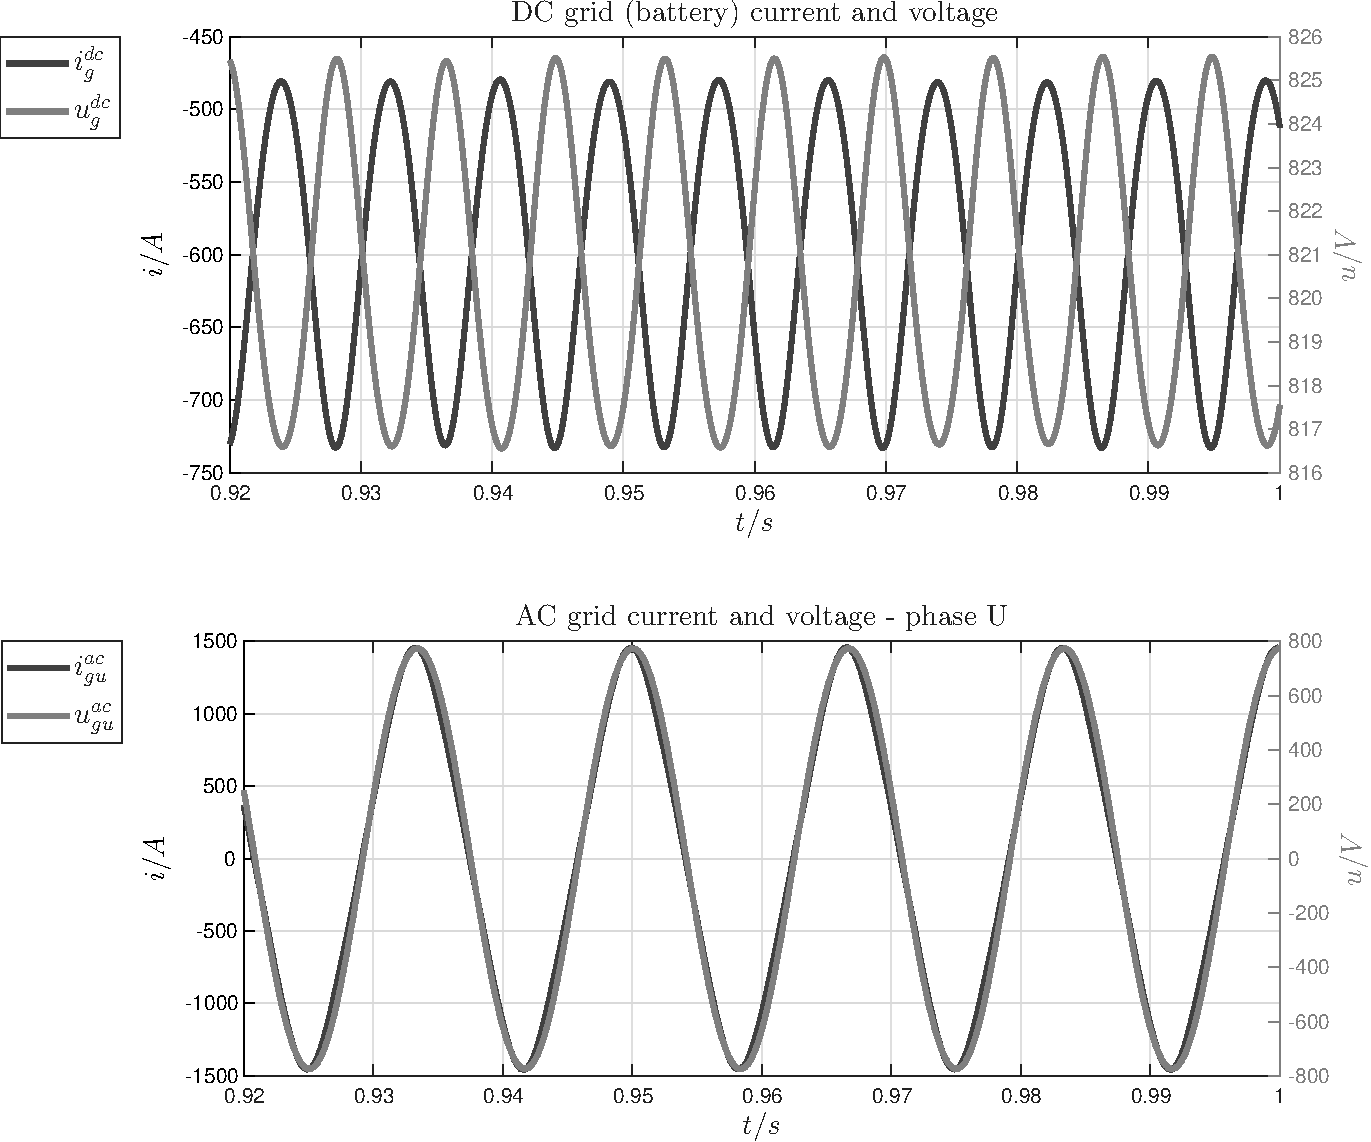
\includegraphics[width=225pt, angle = 0, 
		keepaspectratio]{figures/sim_results/three_phase_dab/dc_ac_grid_voltage_current}
		\captionsetup{width=0.75\textwidth, font=footnotesize}	
		\caption{DC grid current and voltage (top) and AC grid current and voltage (bottom).}
		\label{}
	\end{subfigure}
	\captionsetup{width=0.65\textwidth, font=small}	
	\caption{Three phase DAB with NPC single phase inverter - performance of two stages single phase SST: three phase DAB input/output and grids.}
	\label{}
\end{figure}

\begin{figure}[H]
	\centering
	\begin{subfigure}{0.5\textwidth}
		\centering
		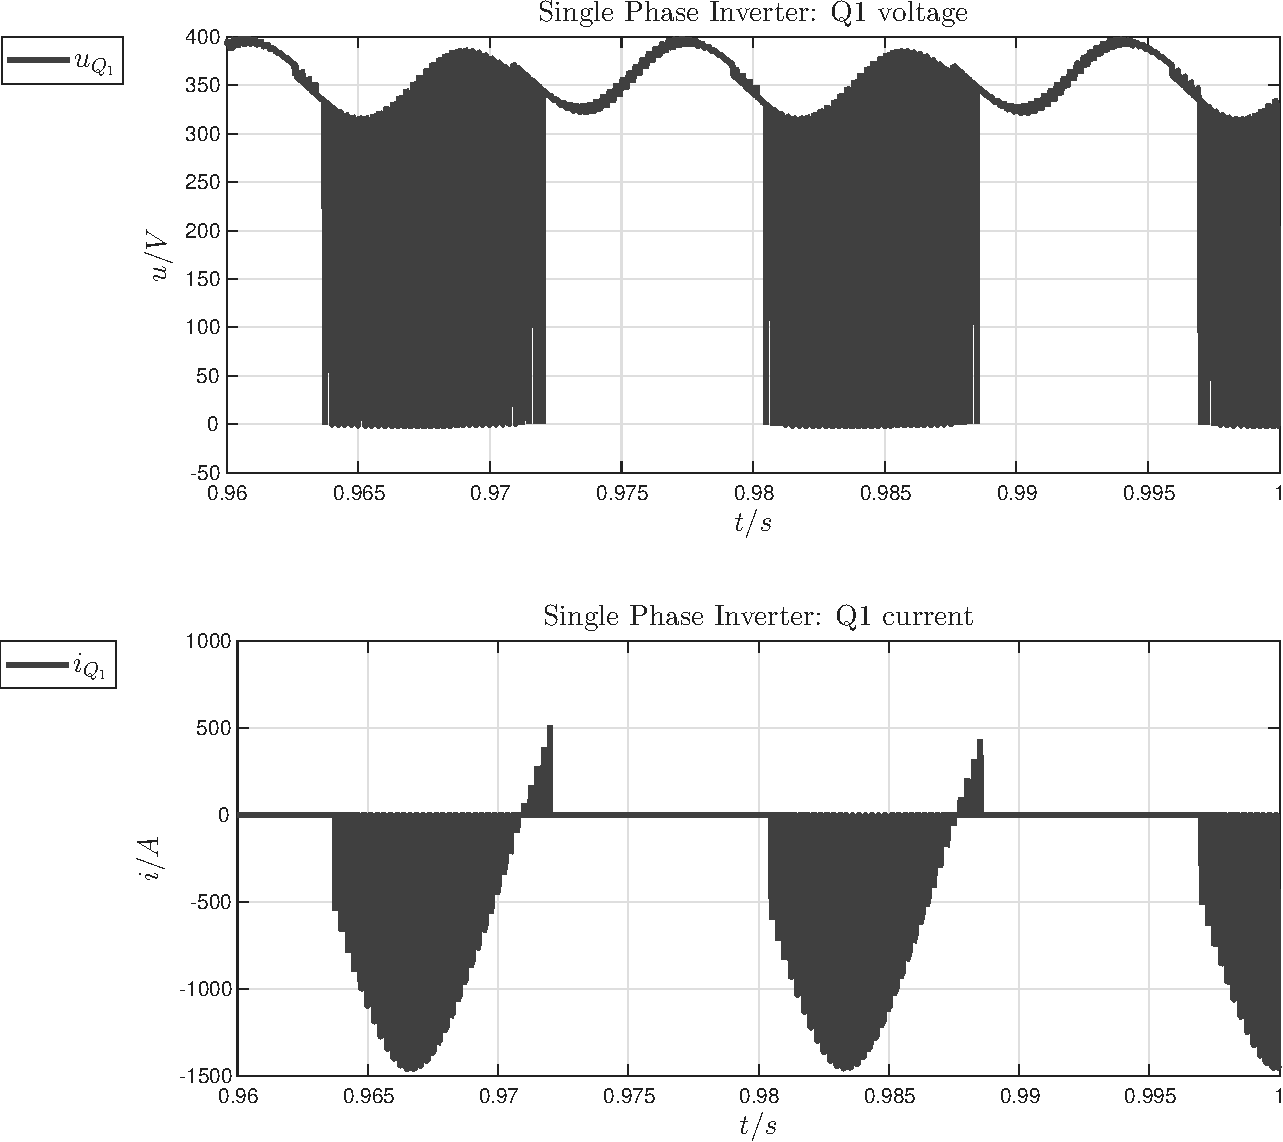
\includegraphics[width =225pt, angle = 0, 
		keepaspectratio]{figures/sim_results/three_phase_dab/single_phase_inverter_Q1}
		\captionsetup{width=0.95\textwidth, font=footnotesize}	
		\caption{Single phase inverter: Q1-IGBT voltage and current. The aim of this image is to proof the effective operative working of the three level NPC single phase inverter. }
		\label{}
	\end{subfigure}%
	\begin{subfigure}{0.5\textwidth}
		\centering
		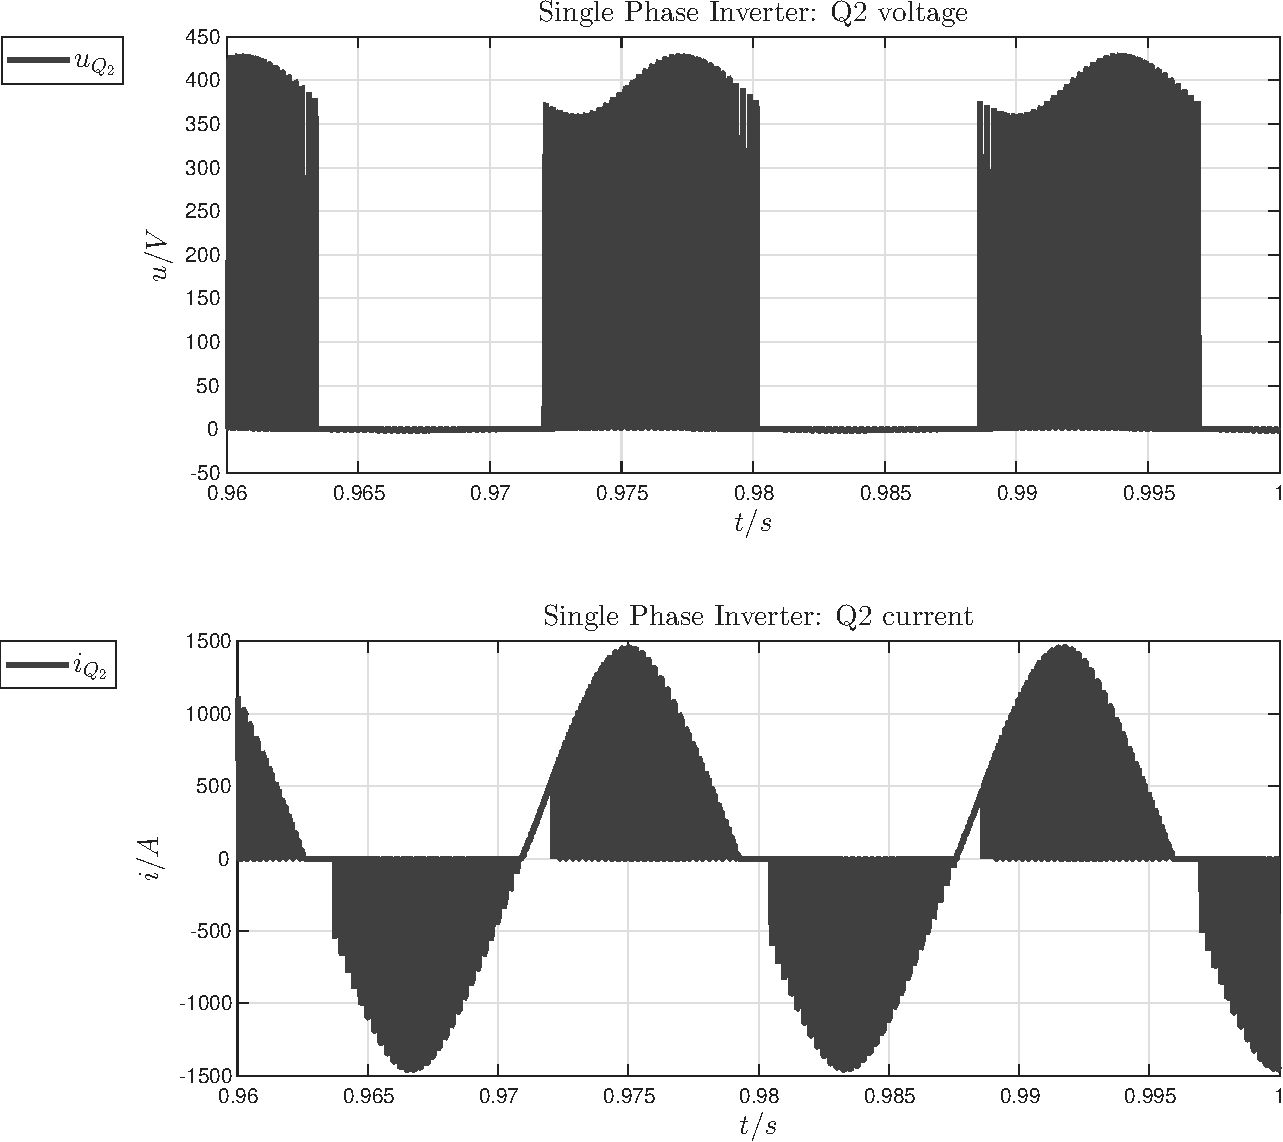
\includegraphics[width =225pt, angle = 0, 
		keepaspectratio]{figures/sim_results/three_phase_dab/single_phase_inverter_Q2}
		\captionsetup{width=0.75\textwidth, font=footnotesize}	
		\caption{Single phase inverter: Q2-IGBT voltage and current. The aim of this image is to proof the effective operative working of the three level NPC single phase inverter.}
		\label{}
	\end{subfigure}
	\captionsetup{width=0.65\textwidth, font=small}	
	\caption{Three phase DAB with NPC single phase inverter - single phase inverter NPC: IGBTs voltage and current.}
	\label{}
\end{figure}

\begin{figure}[H]
	\centering
	\begin{subfigure}{0.5\textwidth}
		\centering
		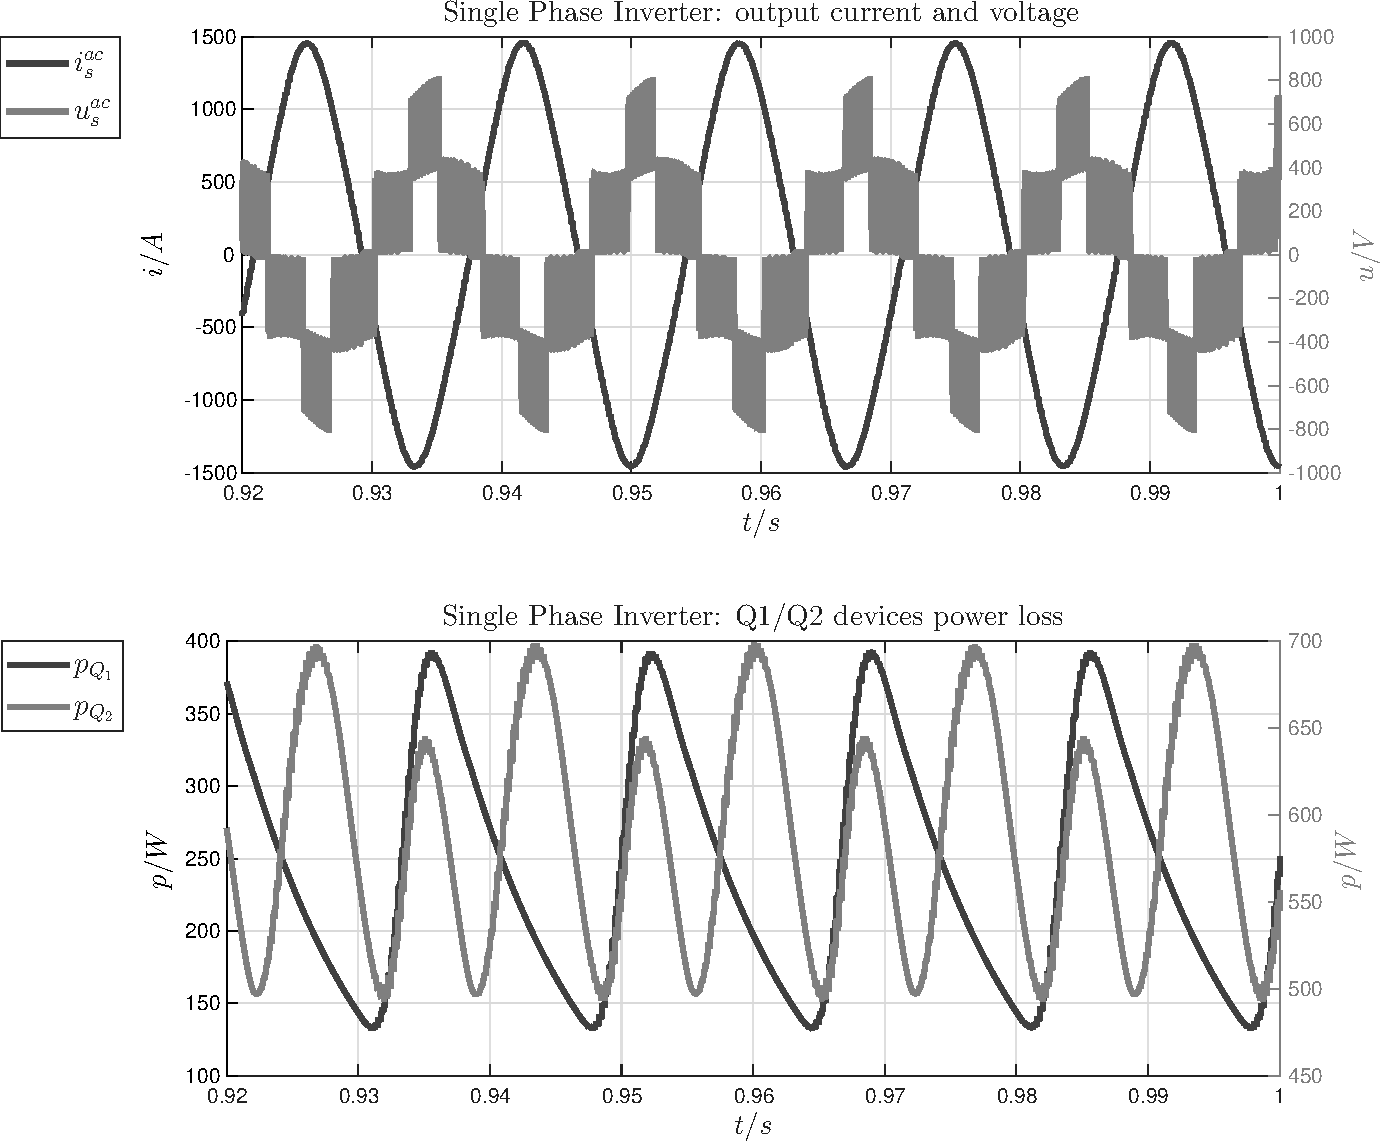
\includegraphics[width =225pt, angle = 0, 
		keepaspectratio]{figures/sim_results/three_phase_dab/single_phase_inverter_performance}
		\captionsetup{width=0.95\textwidth, font=footnotesize}	
		\caption{IGBT Q1 and Q2 power loss (bottom). Single phase output current and voltage, before the output filter (top).}
		\label{}
	\end{subfigure}%
	\begin{subfigure}{0.5\textwidth}
		\centering
		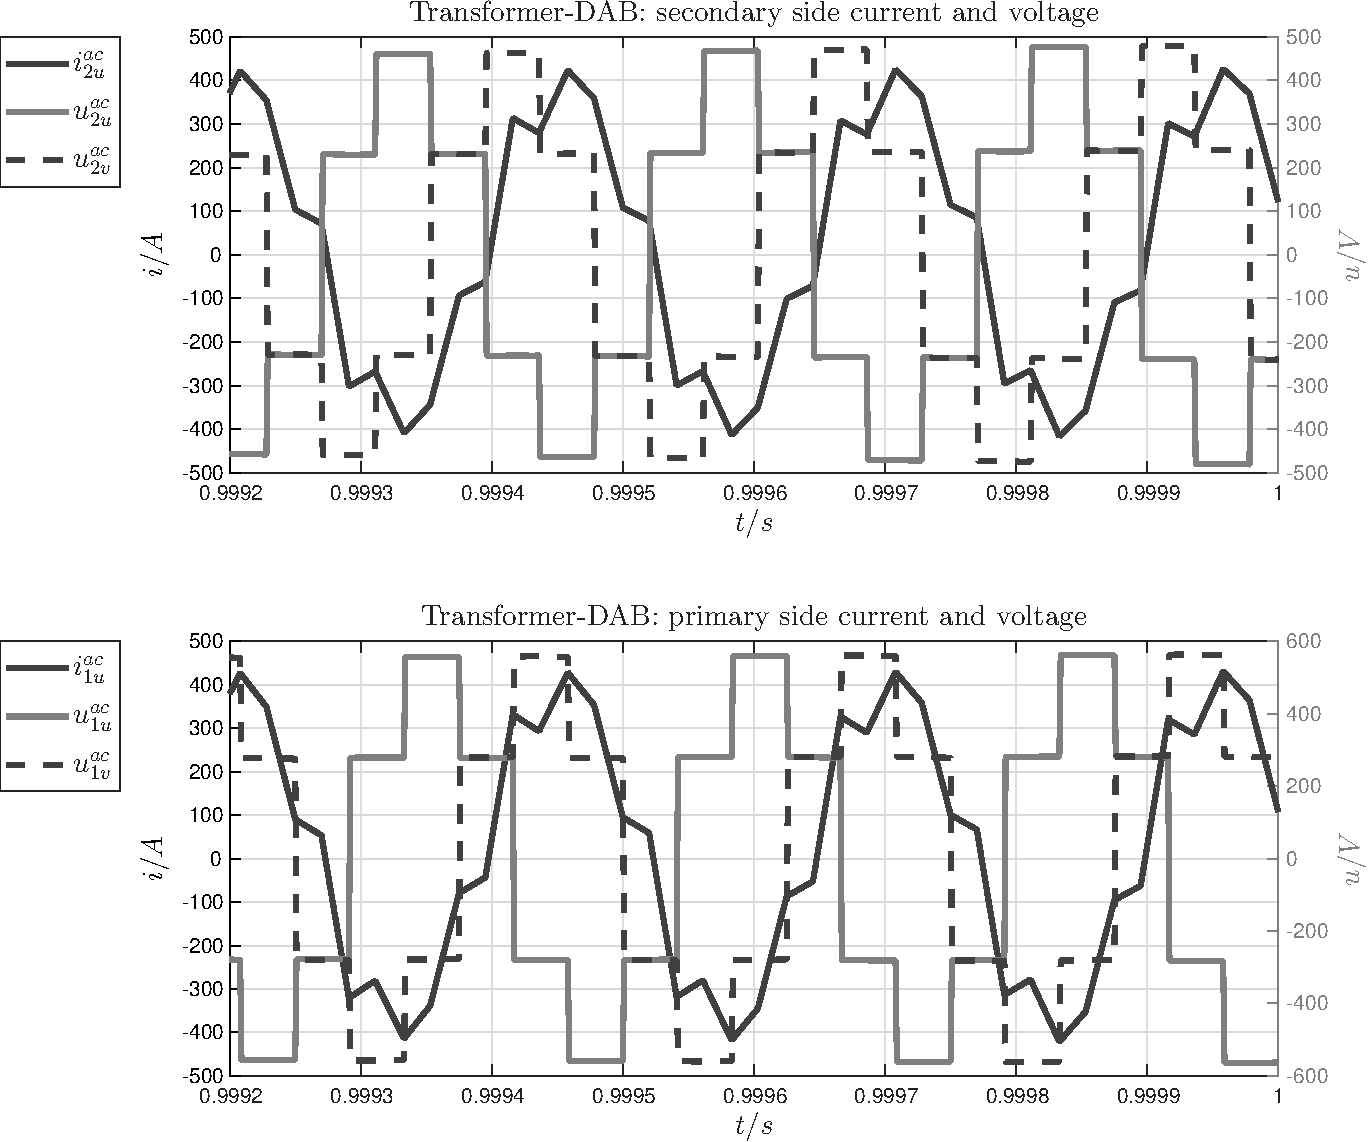
\includegraphics[width =225pt, angle = 0, 
		keepaspectratio]{figures/sim_results/three_phase_dab/dab_transformer_voltage_current}
		\captionsetup{width=0.75\textwidth, font=footnotesize}	
		\caption{Three phase DAB operative condition at nominal flow power.}
		\label{}
	\end{subfigure}
	\captionsetup{width=0.65\textwidth, font=small}	
	\caption{Three phase DAB with NPC single phase inverter - single phase inverter and three phase DAB performances.}
	\label{}
\end{figure}

\begin{figure}[H]
	\centering
	\begin{subfigure}{0.5\textwidth}
		\centering
		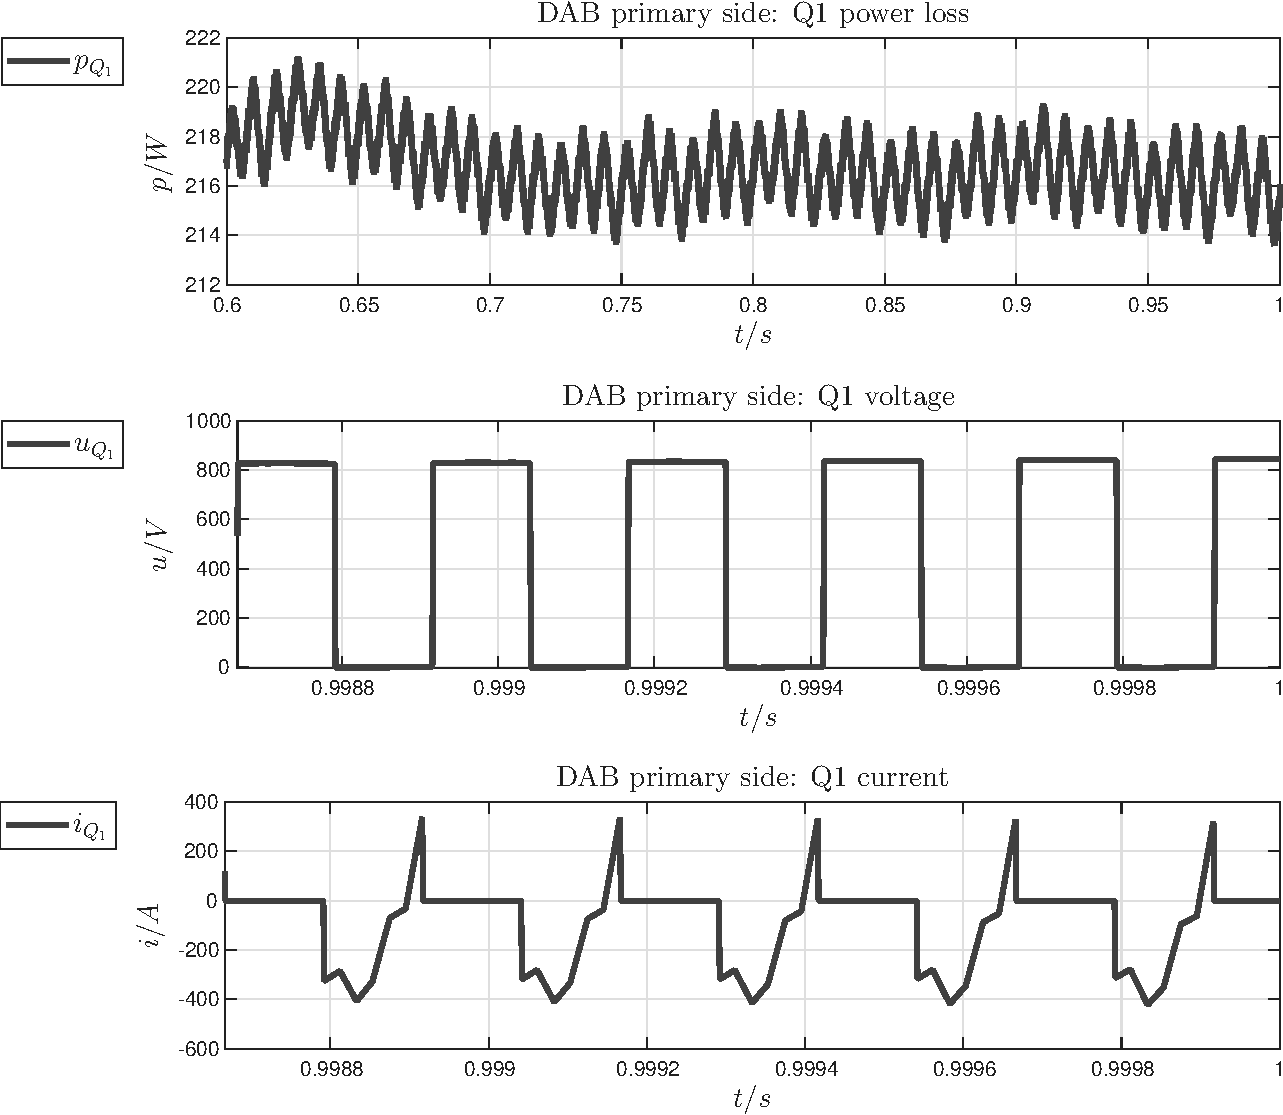
\includegraphics[width =225pt, angle = 0, 
		keepaspectratio]{figures/sim_results/three_phase_dab/DAB_primary_side_Q1}
		\captionsetup{width=0.95\textwidth, font=footnotesize}	
		\caption{Three phase DAB - primary inverter: Q1-MOSFET power loss, voltage and current.}
		\label{}
	\end{subfigure}%
	\begin{subfigure}{0.5\textwidth}
		\centering
		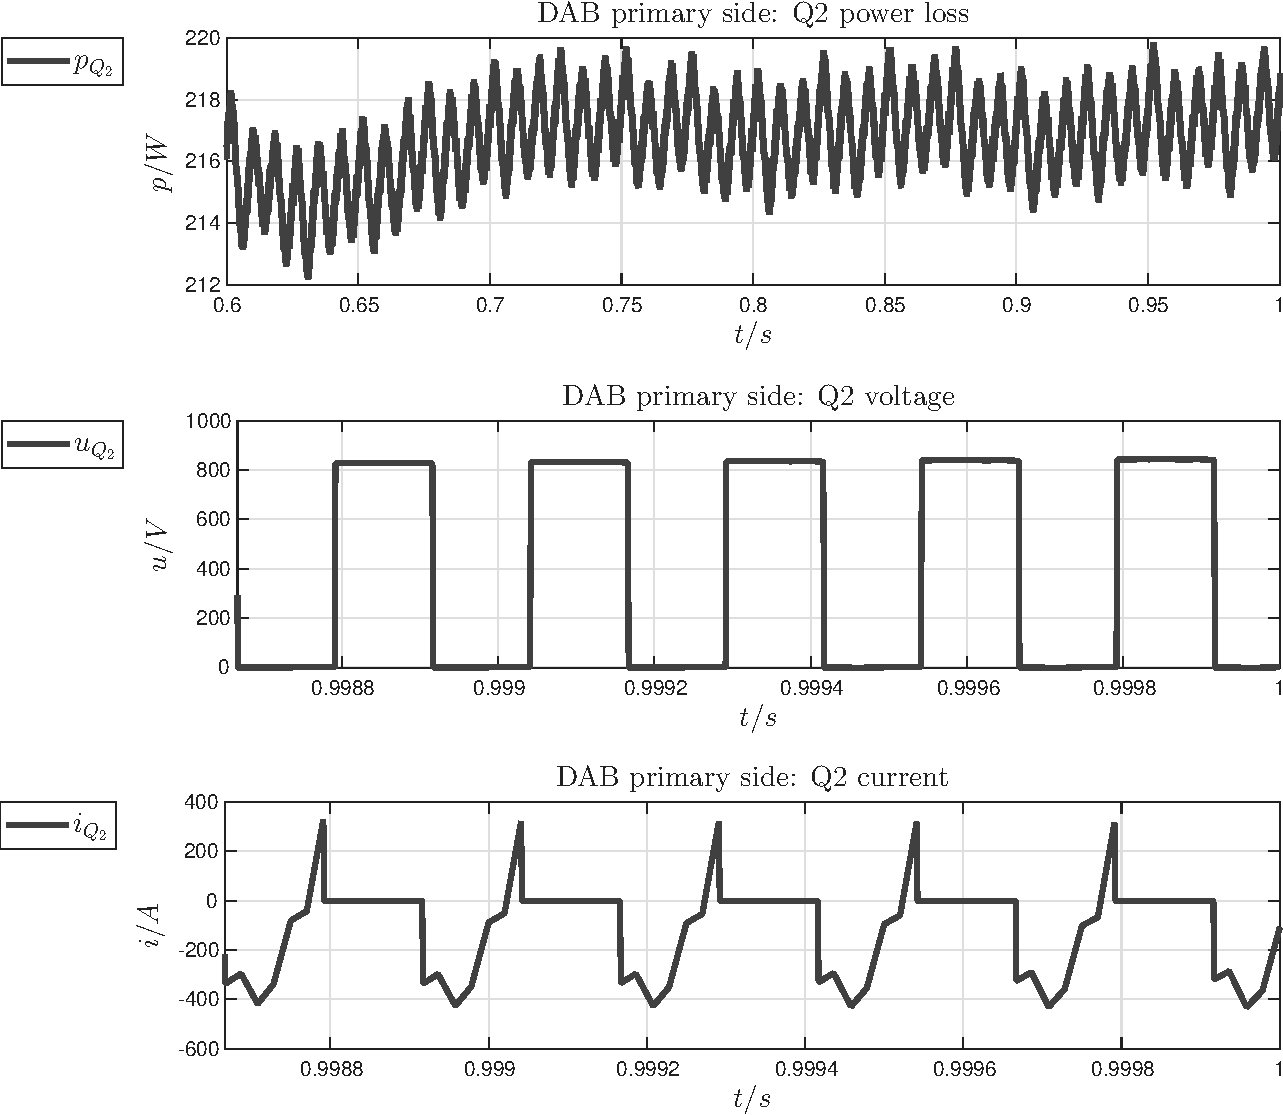
\includegraphics[width =225pt, angle = 0, 
		keepaspectratio]{figures/sim_results/three_phase_dab/DAB_primary_side_Q2}
		\captionsetup{width=0.75\textwidth, font=footnotesize}	
		\caption{Three phase DAB - primary inverter: Q2-MOSFET power loss, voltage and current.}
		\label{}
	\end{subfigure}
	\captionsetup{width=0.65\textwidth, font=small}	
	\caption{Three phase DAB with NPC single phase inverter - primary inverter devices performances.}
	\label{}
\end{figure}

\begin{figure}[H]
	\centering
	\begin{subfigure}{0.5\textwidth}
		\centering
		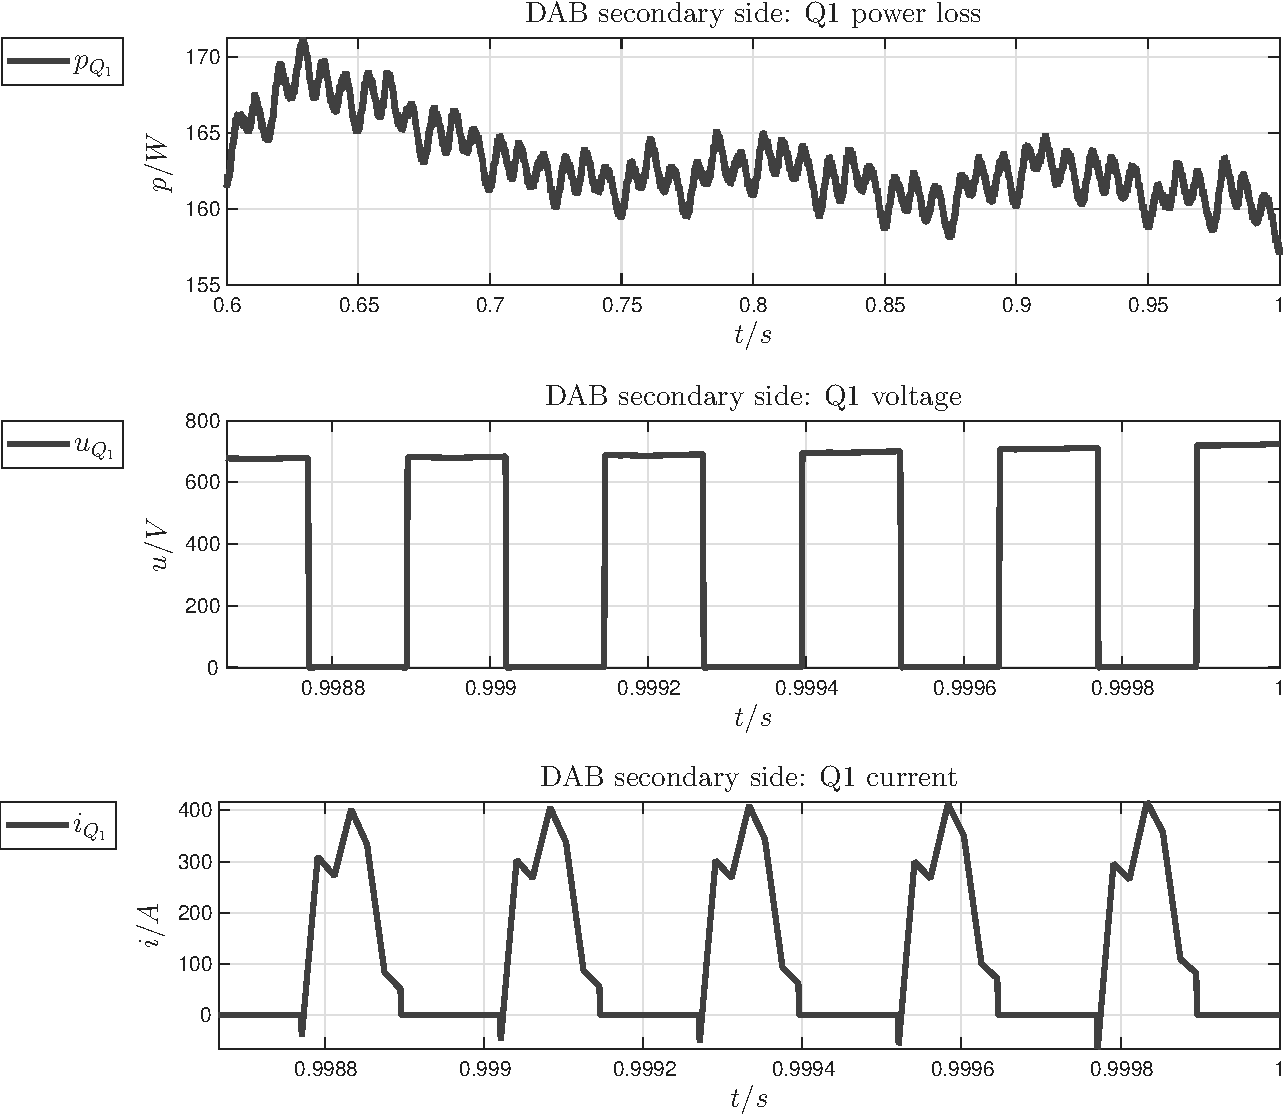
\includegraphics[width =225pt, angle = 0, 
		keepaspectratio]{figures/sim_results/three_phase_dab/DAB_secondary_side_Q1}
		\captionsetup{width=0.95\textwidth, font=footnotesize}	
		\caption{Three phase DAB - secondary inverter: Q1-MOSFET power loss, voltage and current.}
		\label{}
	\end{subfigure}%
	\begin{subfigure}{0.5\textwidth}
		\centering
		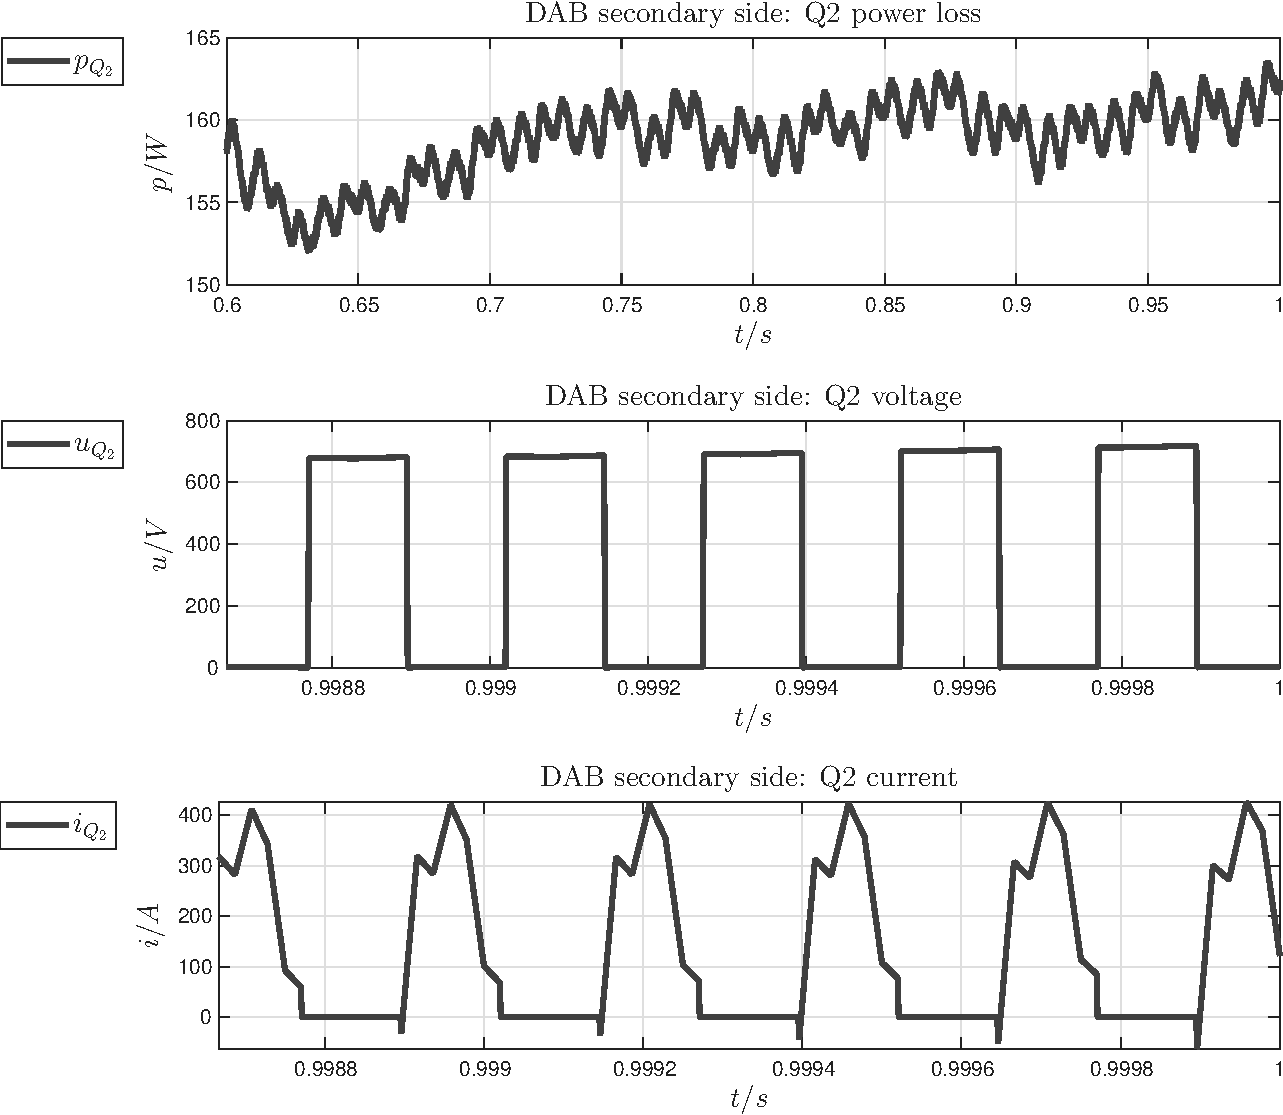
\includegraphics[width =225pt, angle = 0, 
		keepaspectratio]{figures/sim_results/three_phase_dab/DAB_secondary_side_Q2}
		\captionsetup{width=0.75\textwidth, font=footnotesize}	
		\caption{Three phase DAB - secondary inverter: Q2-MOSFET power loss, voltage and current.}
		\label{}
	\end{subfigure}
	\captionsetup{width=0.65\textwidth, font=small}	
	\caption{Three phase DAB with NPC single phase inverter - secondary inverter devices performances.}
	\label{}
\end{figure}

\subsection{SST based on Three Phase DAB and T-Type Single Phase Inverter}
Here performance of the SST based on three phase DAB and a cascade of two three level T-Type single phase inverters.

\noindent\textbf{Remark} - only one single phase has been simulated and total power at DC grid side is resulting in one third than in an equivalent three phase implementation.

\noindent\textbf{Remark} - simulations have been performed under the following condition of grids and load:
\begin{itemize}
	\item[--] DC grid nominal voltage (from Lithium Ion Battery) : $u_{g}^{dc}\Big|_{nom} = \SI{800}{\volt}$;
	\item[--] AC grid nominal voltage : $u_{g}^{ac}\Big|_{nom} = \SI{554}{\volt}$ - rms per phase-centertap;
	\item[--] AC grid load current : $i_{g}^{ac} = \SI{1000}{\ampere}$ - rms;
\end{itemize}

\begin{figure}[H]
	\centering
	\begin{subfigure}{0.5\textwidth}
		\centering
		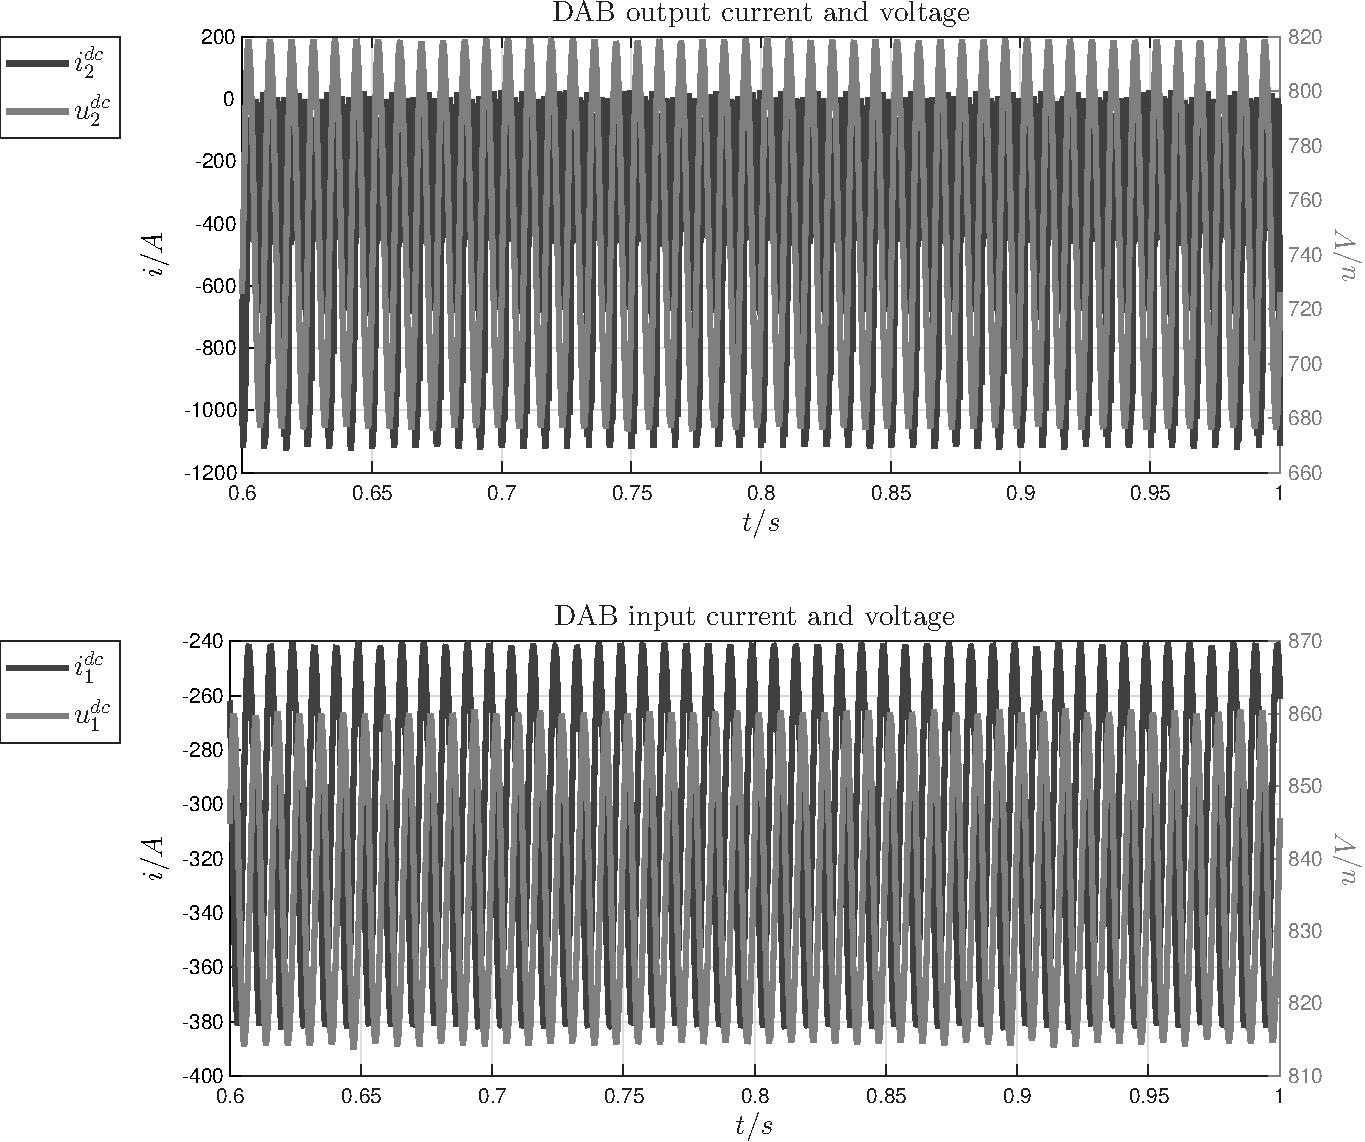
\includegraphics[width =225pt, angle = 0, 
		keepaspectratio]{figures/sim_results/three_phase_dab_with_ttype_inverter/dab_ui_output_input}
		\captionsetup{width=0.95\textwidth, font=footnotesize}	
		\caption{Master three phase DAB input current and voltage (bottom) and outputs (top).}
		\label{}
	\end{subfigure}%
	\begin{subfigure}{0.5\textwidth}
		\centering
		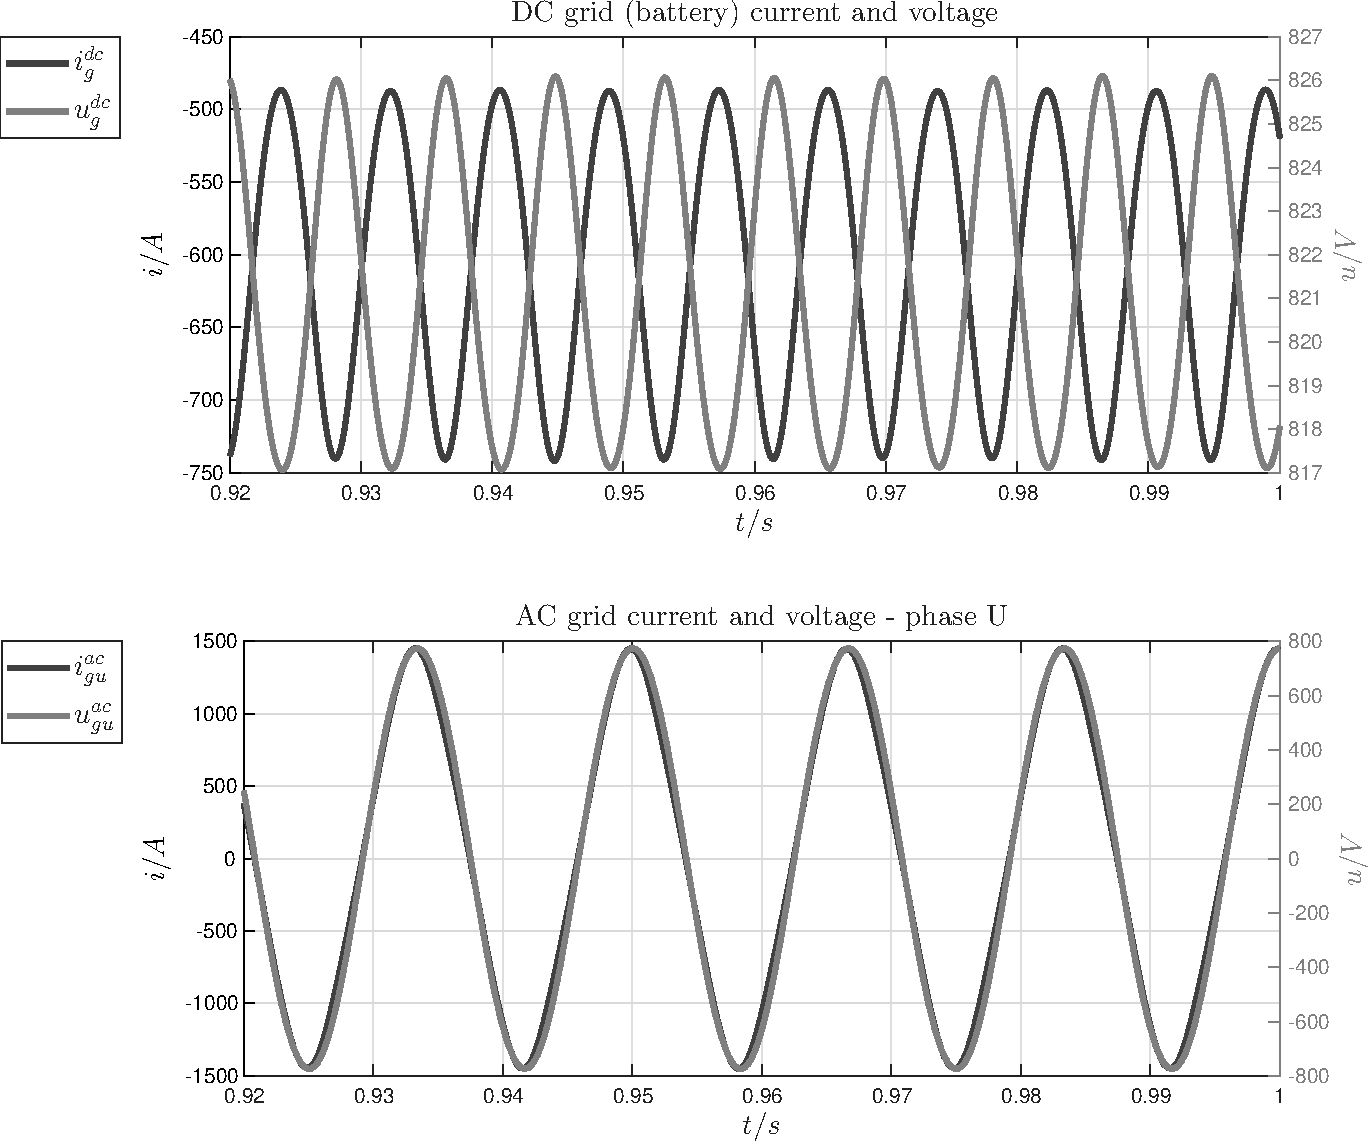
\includegraphics[width=225pt, angle = 0, 
		keepaspectratio]{figures/sim_results/three_phase_dab_with_ttype_inverter/dc_ac_grid_voltage_current}
		\captionsetup{width=0.75\textwidth, font=footnotesize}	
		\caption{DC grid current and voltage (top) and AC grid current and voltage (bottom).}
		\label{}
	\end{subfigure}
	\captionsetup{width=0.65\textwidth, font=small}	
	\caption{Three phase DAB with T-Type single phase inverter - performance of two stages single phase SST: three phase DAB input/output and grids.}
	\label{}
\end{figure}

\begin{figure}[H]
	\centering
	\begin{subfigure}{0.5\textwidth}
		\centering
		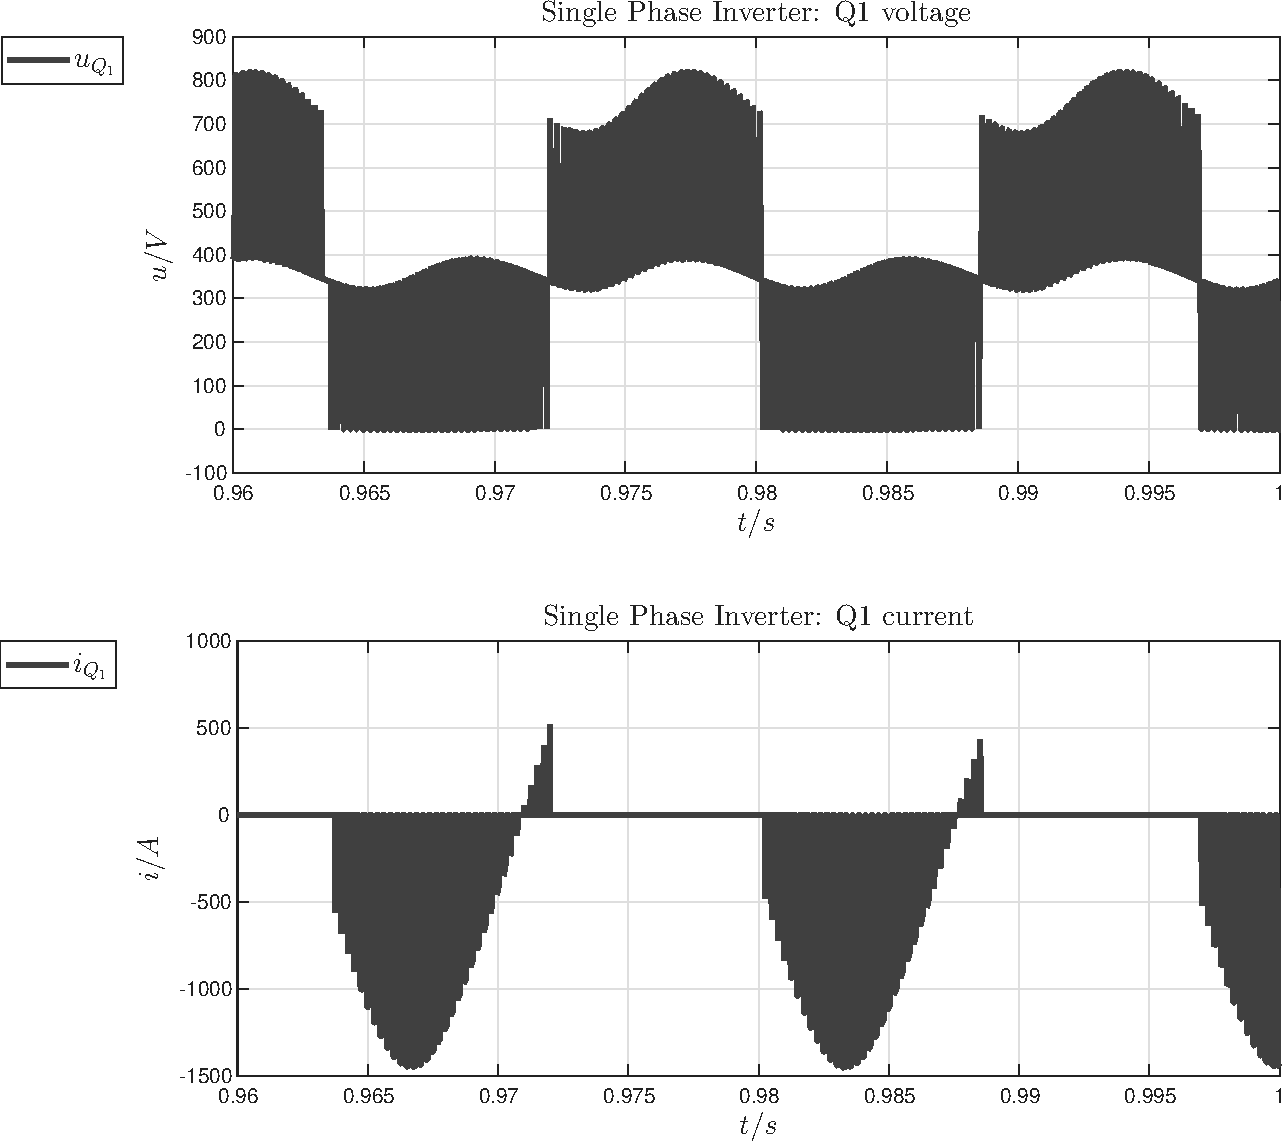
\includegraphics[width =225pt, angle = 0, 
		keepaspectratio]{figures/sim_results/three_phase_dab_with_ttype_inverter/single_phase_inverter_Q1}
		\captionsetup{width=0.95\textwidth, font=footnotesize}	
		\caption{Single phase inverter: Q1-IGBT voltage and current. The aim of this image is to proof the effective operative working of the three level NPC single phase inverter. }
		\label{}
	\end{subfigure}%
	\begin{subfigure}{0.5\textwidth}
		\centering
		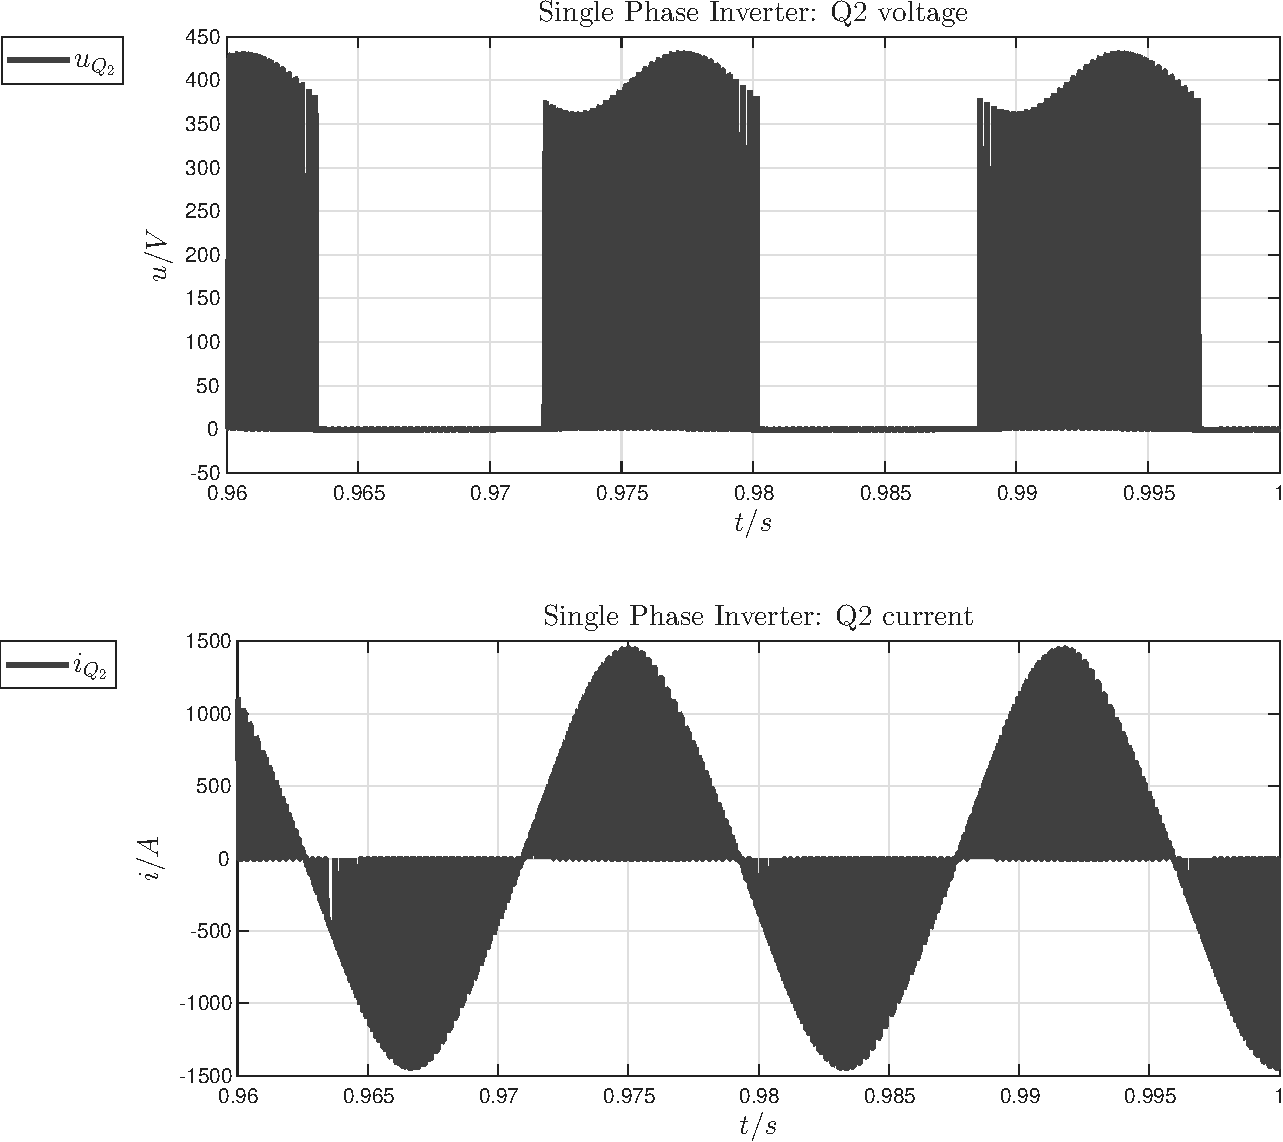
\includegraphics[width =225pt, angle = 0, 
		keepaspectratio]{figures/sim_results/three_phase_dab_with_ttype_inverter/single_phase_inverter_Q2}
		\captionsetup{width=0.75\textwidth, font=footnotesize}	
		\caption{Single phase inverter: Q2-IGBT voltage and current. The aim of this image is to proof the effective operative working of the three level NPC single phase inverter.}
		\label{}
	\end{subfigure}
	\captionsetup{width=0.65\textwidth, font=small}	
	\caption{Three phase DAB with T-Type single phase inverter - single phase inverter T-Type: IGBTs voltage and current.}
	\label{}
\end{figure}

\begin{figure}[H]
	\centering
	\begin{subfigure}{0.5\textwidth}
		\centering
		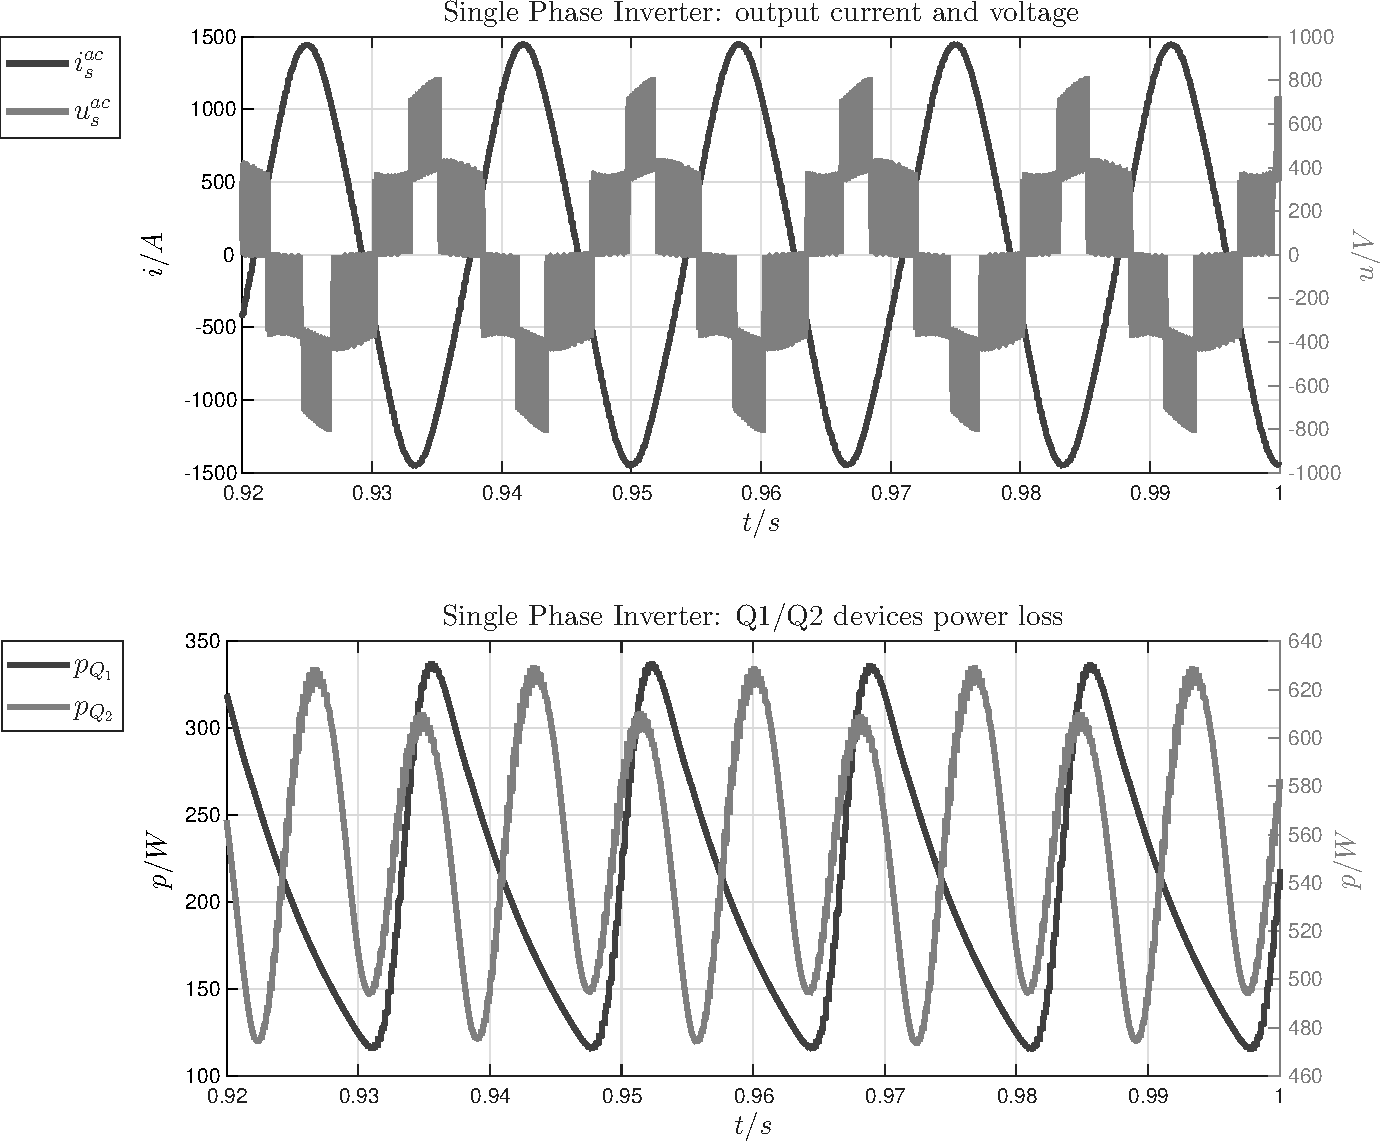
\includegraphics[width =225pt, angle = 0, 
		keepaspectratio]{figures/sim_results/three_phase_dab_with_ttype_inverter/single_phase_inverter_performance}
		\captionsetup{width=0.95\textwidth, font=footnotesize}	
		\caption{IGBT Q1 and Q2 power loss (bottom). Single phase output current and voltage, before the output filter (top).}
		\label{}
	\end{subfigure}%
	\begin{subfigure}{0.5\textwidth}
		\centering
		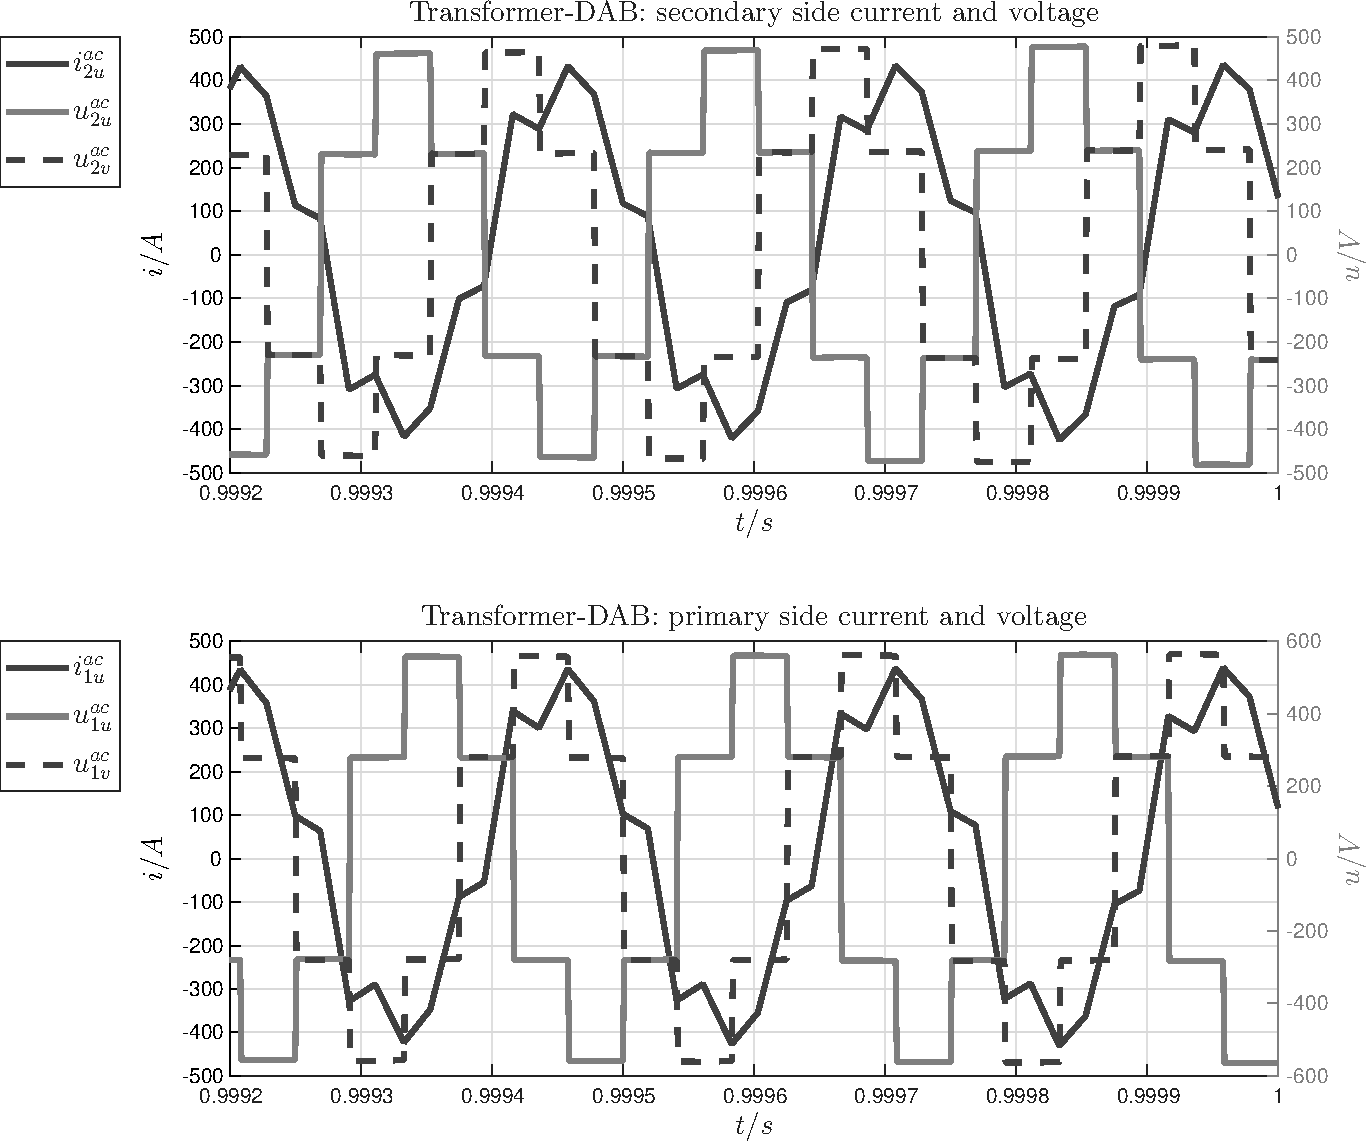
\includegraphics[width =225pt, angle = 0, 
		keepaspectratio]{figures/sim_results/three_phase_dab_with_ttype_inverter/dab_transformer_voltage_current}
		\captionsetup{width=0.75\textwidth, font=footnotesize}	
		\caption{Three phase DAB operative condition at nominal flow power.}
		\label{}
	\end{subfigure}
	\captionsetup{width=0.65\textwidth, font=small}	
	\caption{Three phase DAB with T-Type single phase inverter - single phase inverter and three phase DAB performances.}
	\label{}
\end{figure}

\begin{figure}[H]
	\centering
	\begin{subfigure}{0.5\textwidth}
		\centering
		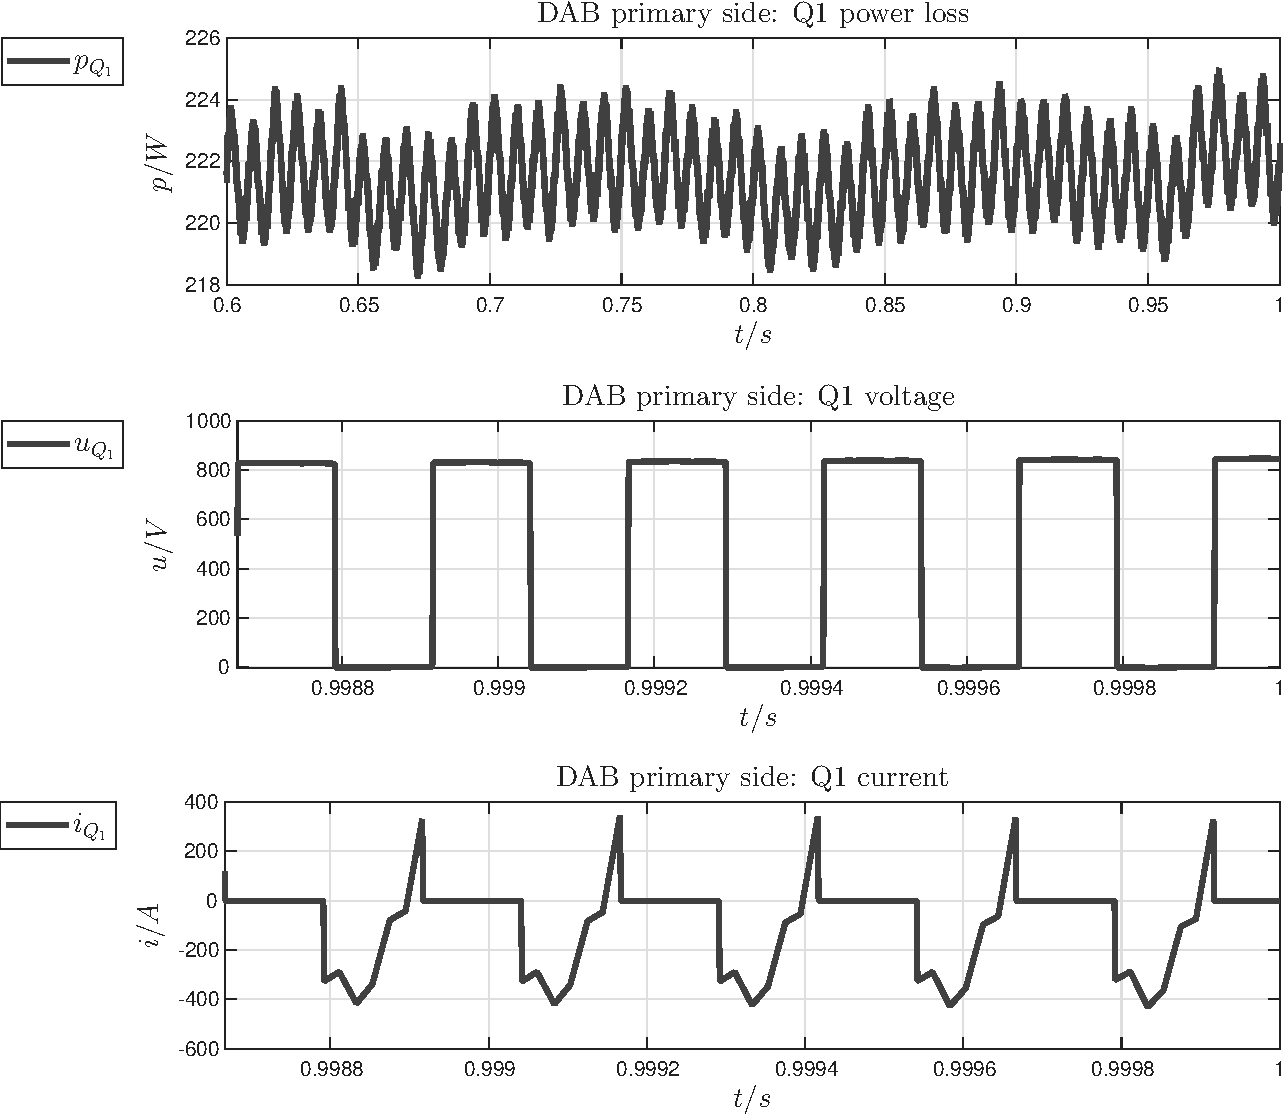
\includegraphics[width =225pt, angle = 0, 
		keepaspectratio]{figures/sim_results/three_phase_dab_with_ttype_inverter/DAB_primary_side_Q1}
		\captionsetup{width=0.95\textwidth, font=footnotesize}	
		\caption{Three phase DAB - primary inverter: Q1-MOSFET power loss, voltage and current.}
		\label{}
	\end{subfigure}%
	\begin{subfigure}{0.5\textwidth}
		\centering
		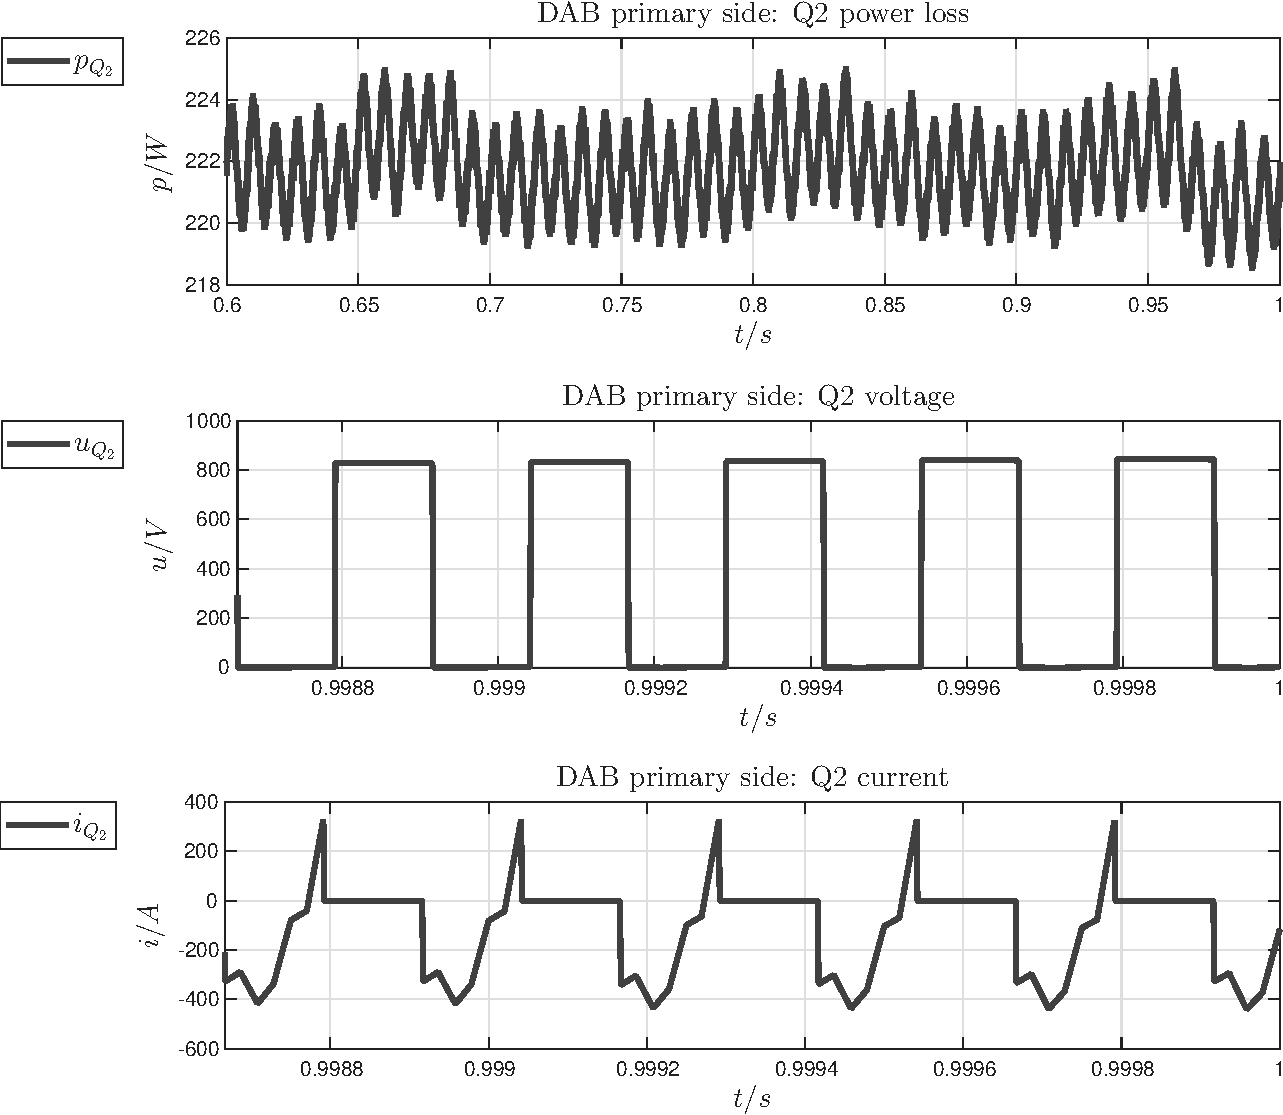
\includegraphics[width =225pt, angle = 0, 
		keepaspectratio]{figures/sim_results/three_phase_dab_with_ttype_inverter/DAB_primary_side_Q2}
		\captionsetup{width=0.75\textwidth, font=footnotesize}	
		\caption{Three phase DAB - primary inverter: Q2-MOSFET power loss, voltage and current.}
		\label{}
	\end{subfigure}
	\captionsetup{width=0.65\textwidth, font=small}	
	\caption{Three phase DAB with T-Type single phase inverter - primary inverter devices performances.}
	\label{}
\end{figure}

\begin{figure}[H]
	\centering
	\begin{subfigure}{0.5\textwidth}
		\centering
		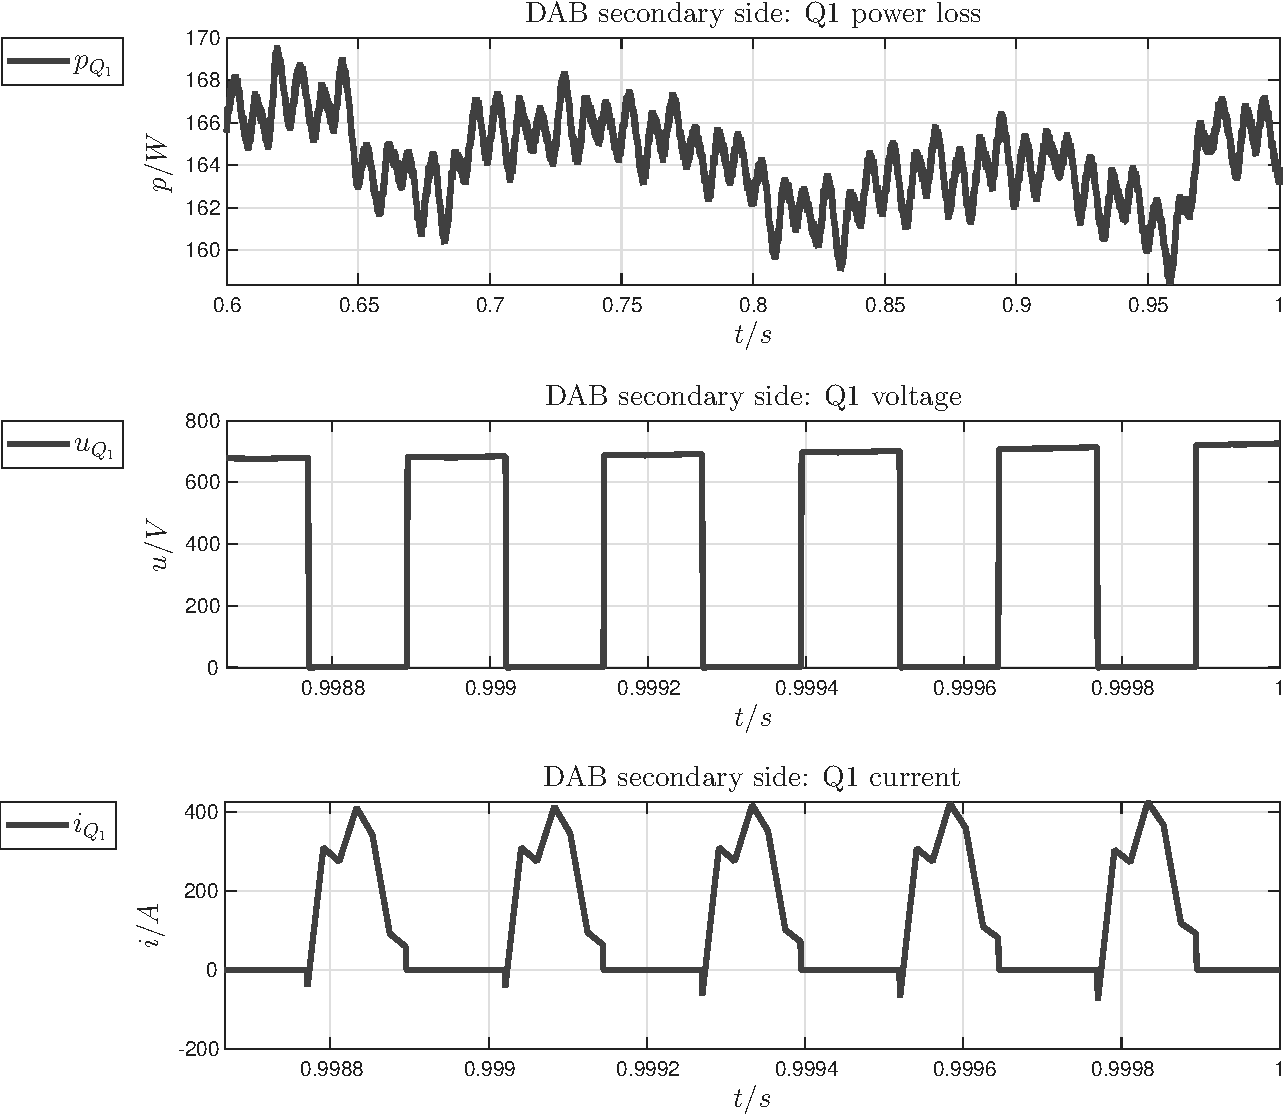
\includegraphics[width =225pt, angle = 0, 
		keepaspectratio]{figures/sim_results/three_phase_dab_with_ttype_inverter/DAB_secondary_side_Q1}
		\captionsetup{width=0.95\textwidth, font=footnotesize}	
		\caption{Three phase DAB - secondary inverter: Q1-MOSFET power loss, voltage and current.}
		\label{}
	\end{subfigure}%
	\begin{subfigure}{0.5\textwidth}
		\centering
		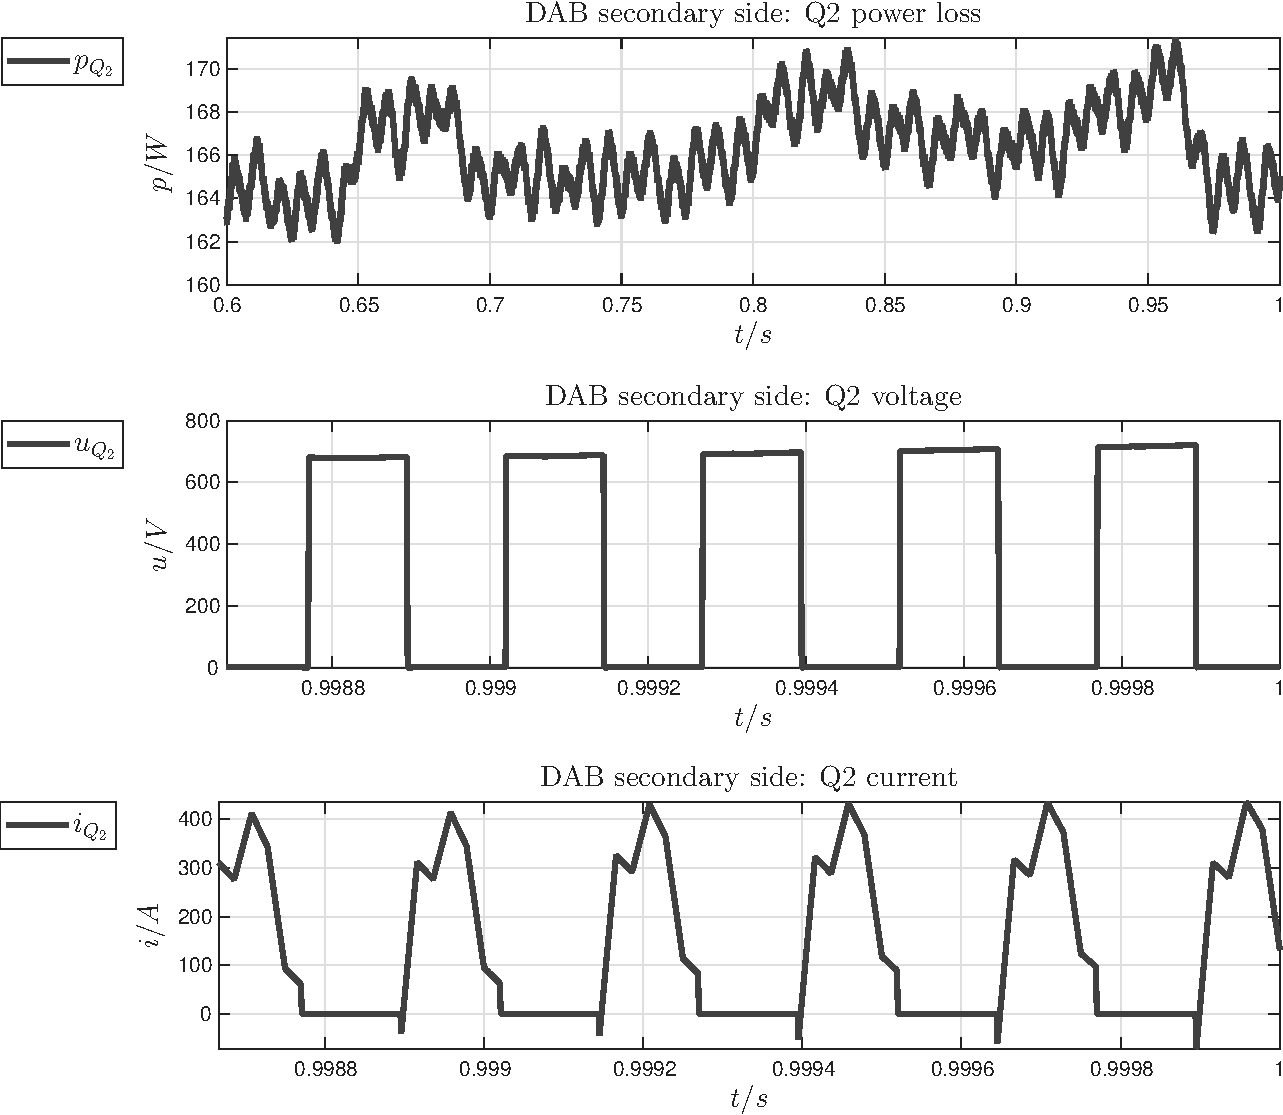
\includegraphics[width =225pt, angle = 0, 
		keepaspectratio]{figures/sim_results/three_phase_dab_with_ttype_inverter/DAB_secondary_side_Q2}
		\captionsetup{width=0.75\textwidth, font=footnotesize}	
		\caption{Three phase DAB - secondary inverter: Q2-MOSFET power loss, voltage and current.}
		\label{}
	\end{subfigure}
	\captionsetup{width=0.65\textwidth, font=small}	
	\caption{Three phase DAB with T-Type single phase inverter - secondary inverter devices performances.}
	\label{}
\end{figure}


\subsection{SST based on Single Phase CLLC and NPC Single Phase Inverter}
\label{sec:sim_cllc}
In this section the performance of the CLLC has been investigated. The control strategy of the CLLC DCDC converter has been assumed as follows
\begin{itemize}
	\item[--] single phase CLLC is operating at constant frequency of $f_{\text{llc}} = \SI{13}{\kilo\hertz}$;
	\item[--] power flow direction as well as amplitude is controlled by phase shift between primary and secondary side H-bridges;
	\item[--] the above control law keep the CLLC conversion in a constant condition of zero current switching;	
\end{itemize}

\begin{figure}[H]
	\centering
	\begin{subfigure}{0.5\textwidth}
		\centering
		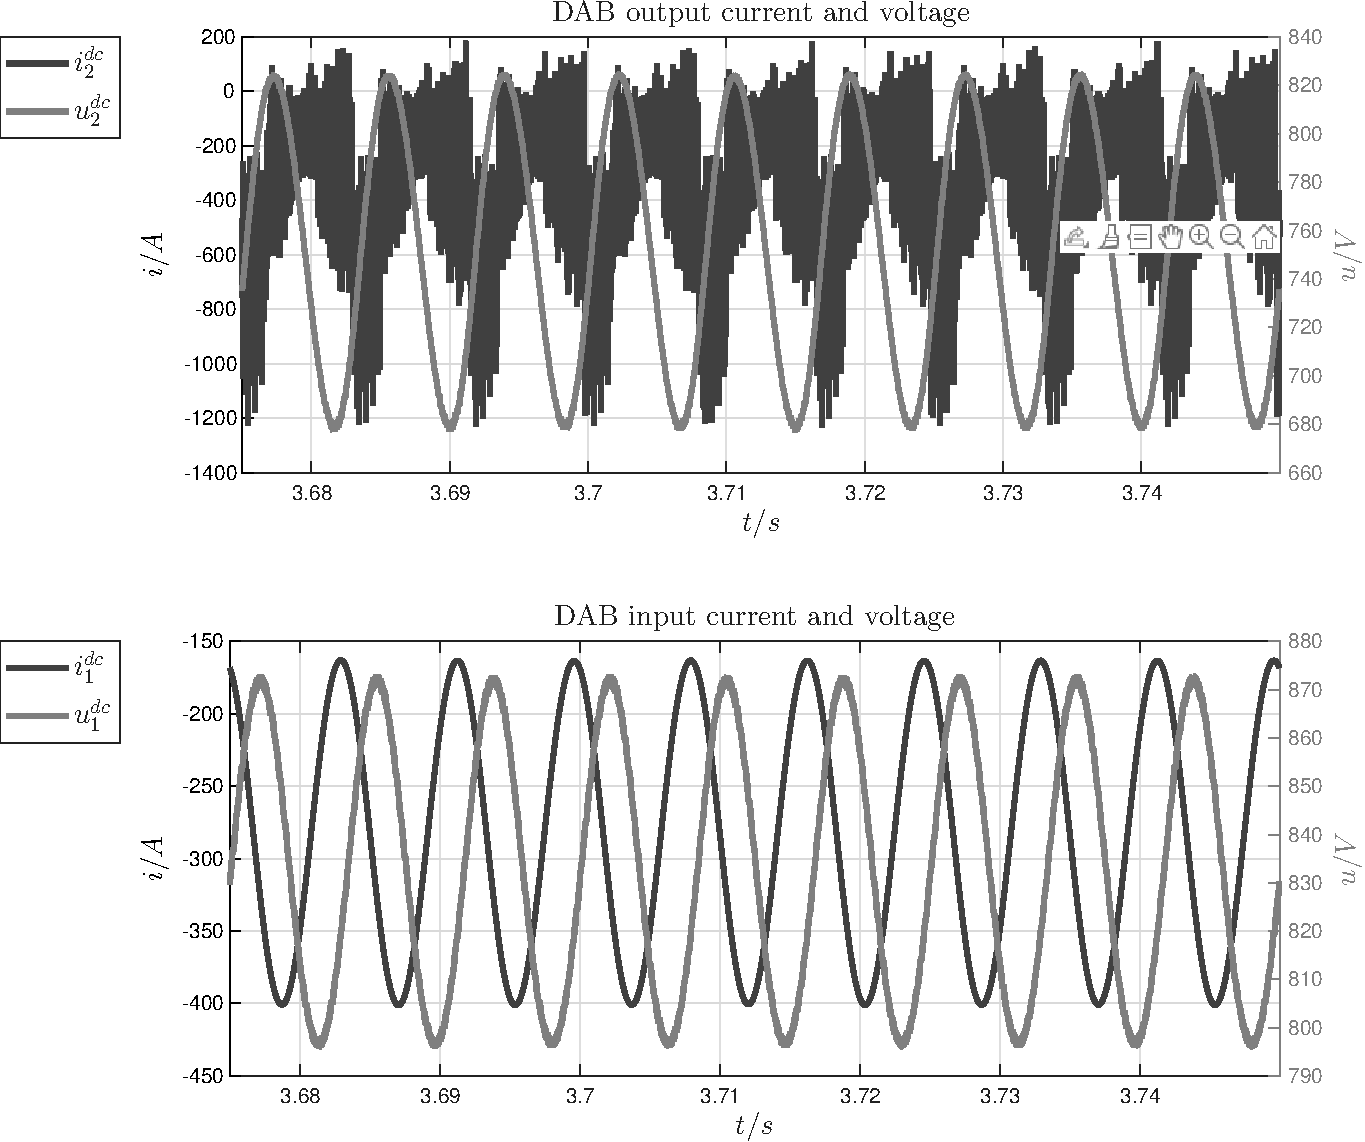
\includegraphics[width =225pt, angle = 0, 
		keepaspectratio]{figures/sim_results/single_phase_llc/dab_ui_output_input}
		\captionsetup{width=0.95\textwidth, font=footnotesize}	
		\caption{Single phase CLLC with NPC single phase inverter - Master single phase CLLC input current and voltage (bottom) and outputs (top).}
		\label{}
	\end{subfigure}%
	\begin{subfigure}{0.5\textwidth}
		\centering
		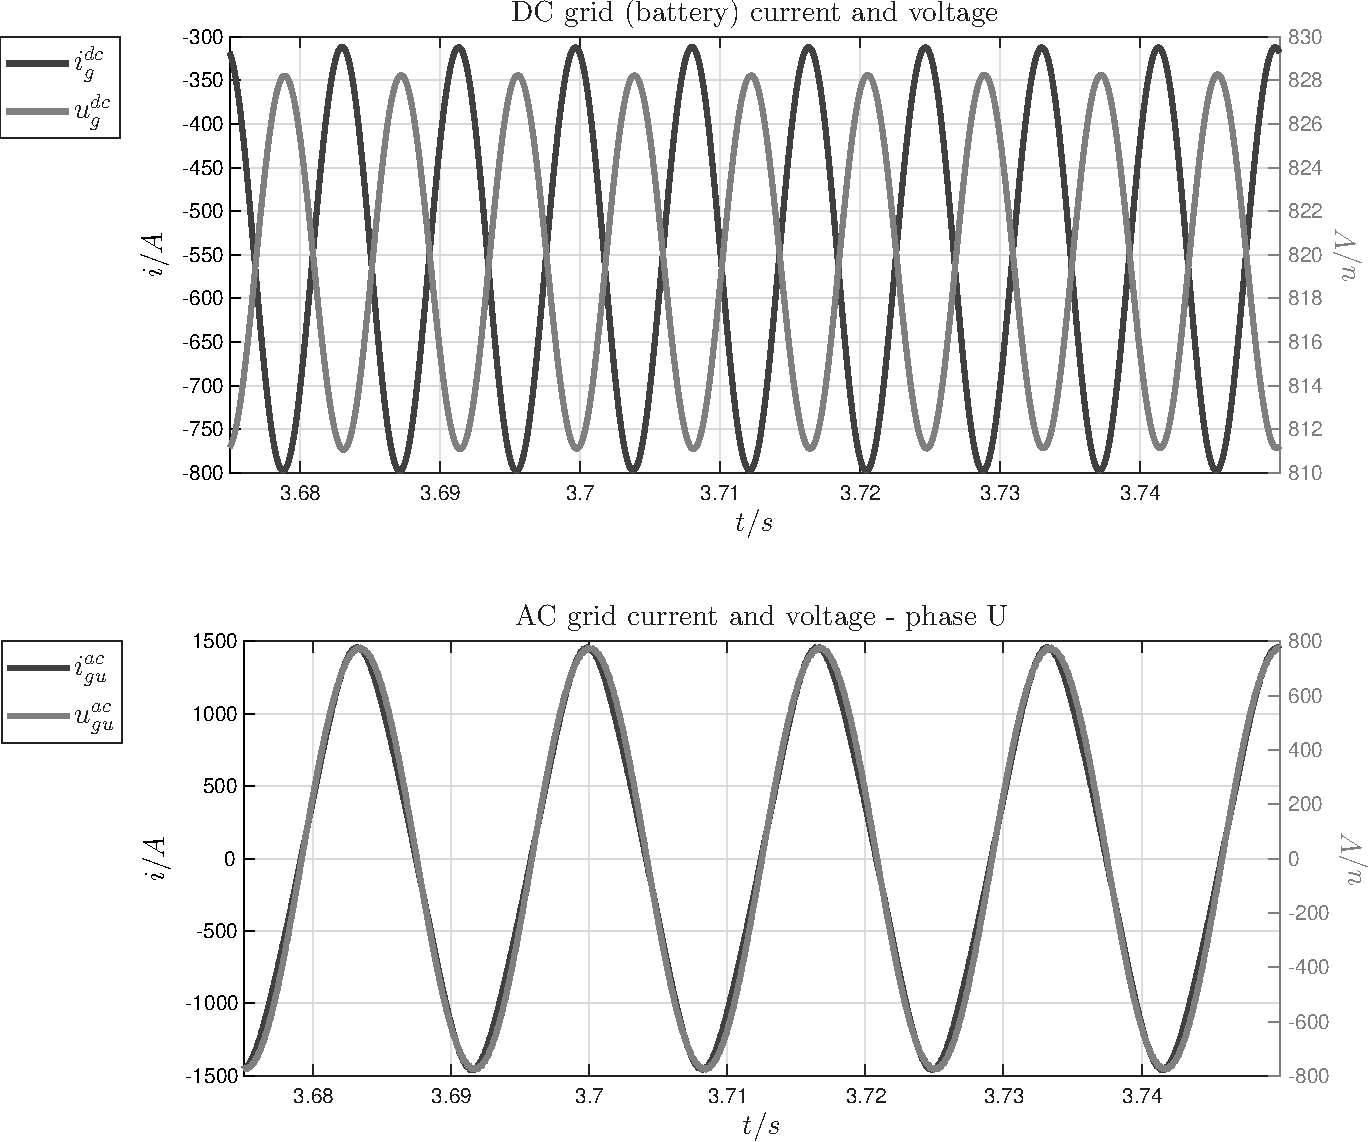
\includegraphics[width =225pt, angle = 0, 
		keepaspectratio]{figures/sim_results/single_phase_llc/dc_ac_grid_voltage_current}
		\captionsetup{width=0.75\textwidth, font=footnotesize}	
		\caption{DC grid current and voltage (top) and AC grid current and voltage (bottom).}	
		\label{}
	\end{subfigure}
	\captionsetup{width=0.65\textwidth, font=small}	
	\caption{Single phase CLLC with NPC single phase inverter - performance of two stages single phase SST: single phase CLLC input/output and grids.}
	\label{}
\end{figure}

\begin{figure}[H]
	\centering
	\begin{subfigure}{0.5\textwidth}
		\centering
		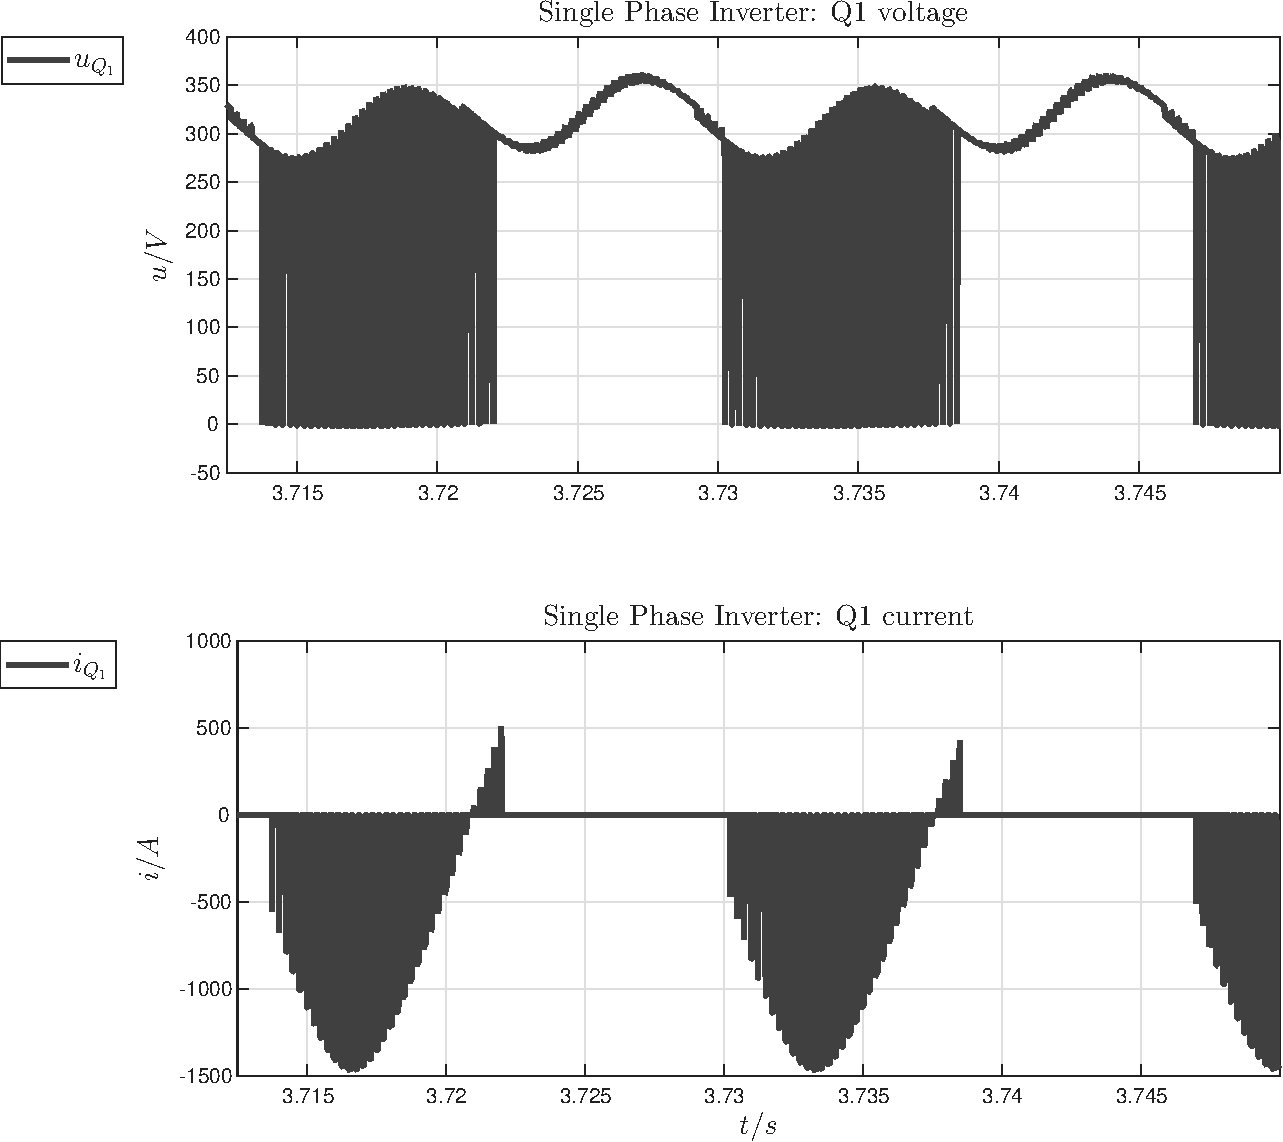
\includegraphics[width =225pt, angle = 0, 
		keepaspectratio]{figures/sim_results/single_phase_llc/single_phase_inverter_Q1}
		\captionsetup{width=0.95\textwidth, font=footnotesize}	
		\caption{Single phase inverter: Q1-IGBT voltage and current. The aim of this image is to proof the effective operative working of the three level NPC single phase inverter.}
		\label{}
	\end{subfigure}%
	\begin{subfigure}{0.5\textwidth}
		\centering
		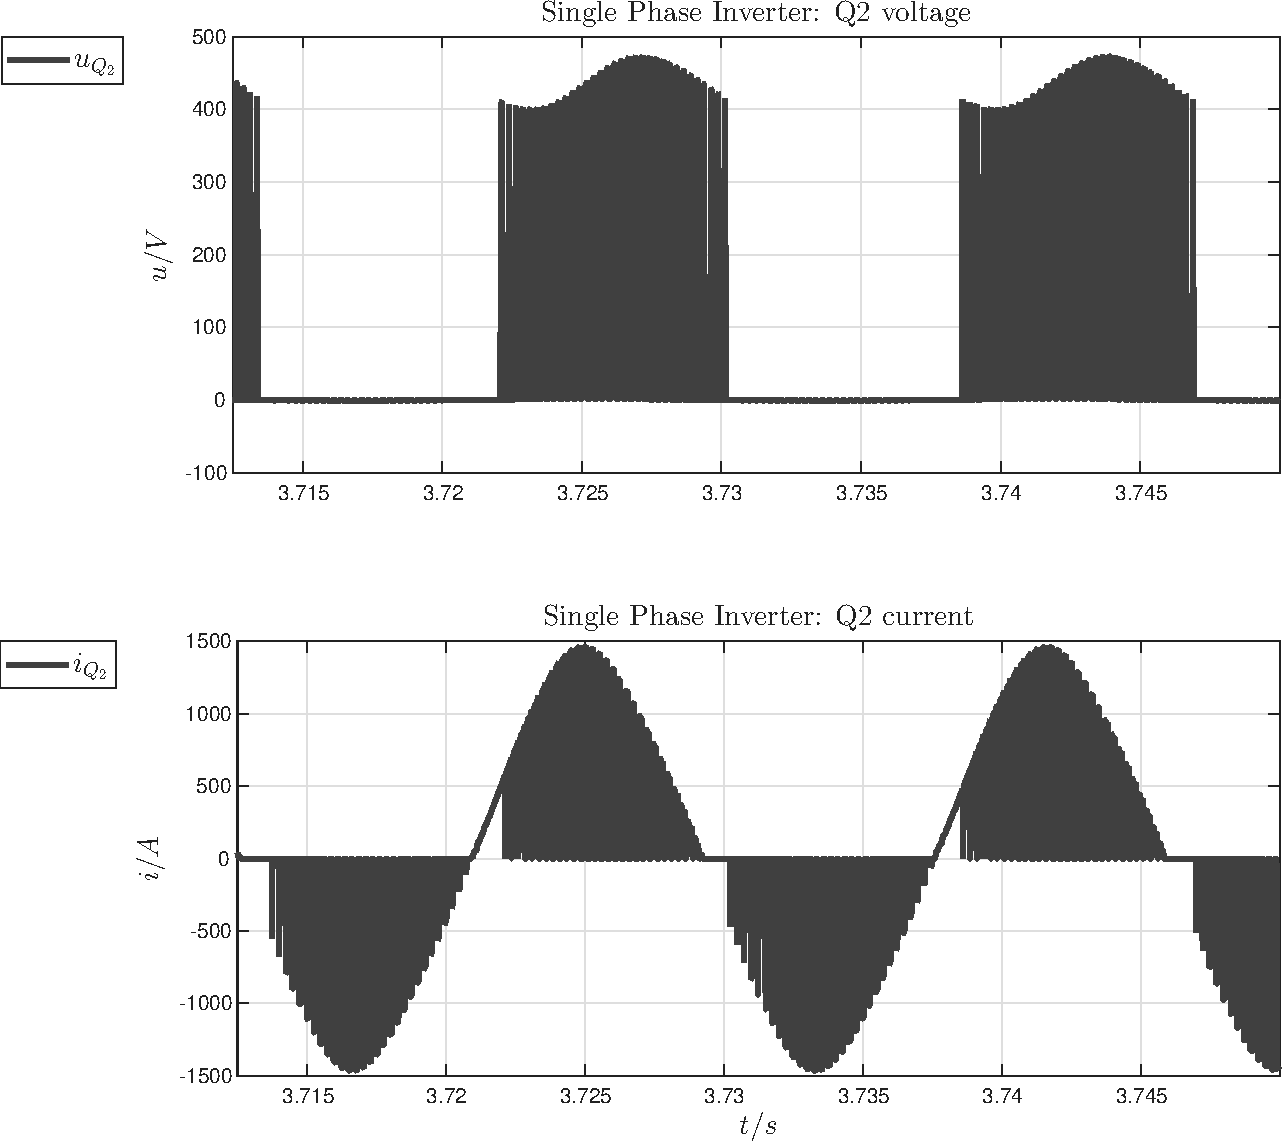
\includegraphics[width =225pt, angle = 0, 
		keepaspectratio]{figures/sim_results/single_phase_llc/single_phase_inverter_Q2}
		\captionsetup{width=0.75\textwidth, font=footnotesize}	
		\caption{Single phase inverter: Q2-IGBT voltage and current. The aim of this image is to proof the effective operative working of the three level NPC single phase inverter.}
		\label{}
	\end{subfigure}
	\captionsetup{width=0.65\textwidth, font=small}	
	\caption{Single phase CLLC with NPC single phase inverter - single phase inverter NPC: IGBTs voltage and current.}
	\label{}
\end{figure}


\begin{figure}[H]
	\centering
	\begin{subfigure}{0.5\textwidth}
		\centering
		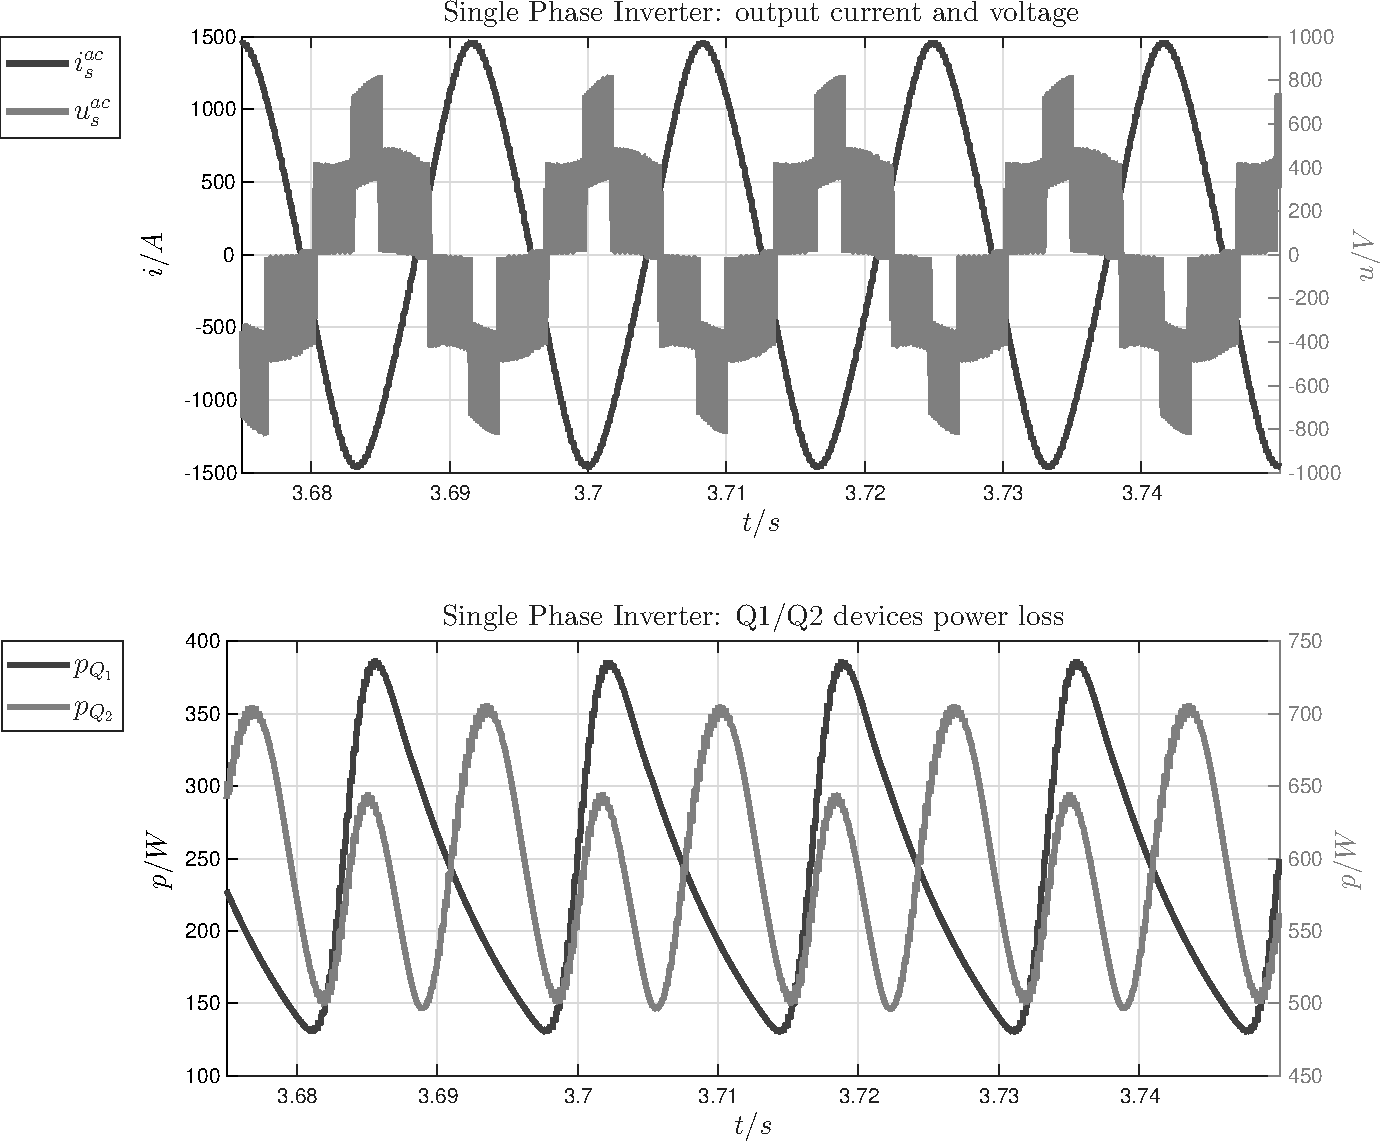
\includegraphics[width =225pt, angle = 0, 
		keepaspectratio]{figures/sim_results/single_phase_llc/single_phase_inverter_performance}
		\captionsetup{width=0.95\textwidth, font=footnotesize}	
		\caption{IGBT Q1 and Q2 power loss (bottom). Single phase output current and voltage, before the output filter (top).}
		\label{}
	\end{subfigure}%
	\begin{subfigure}{0.5\textwidth}
		\centering
		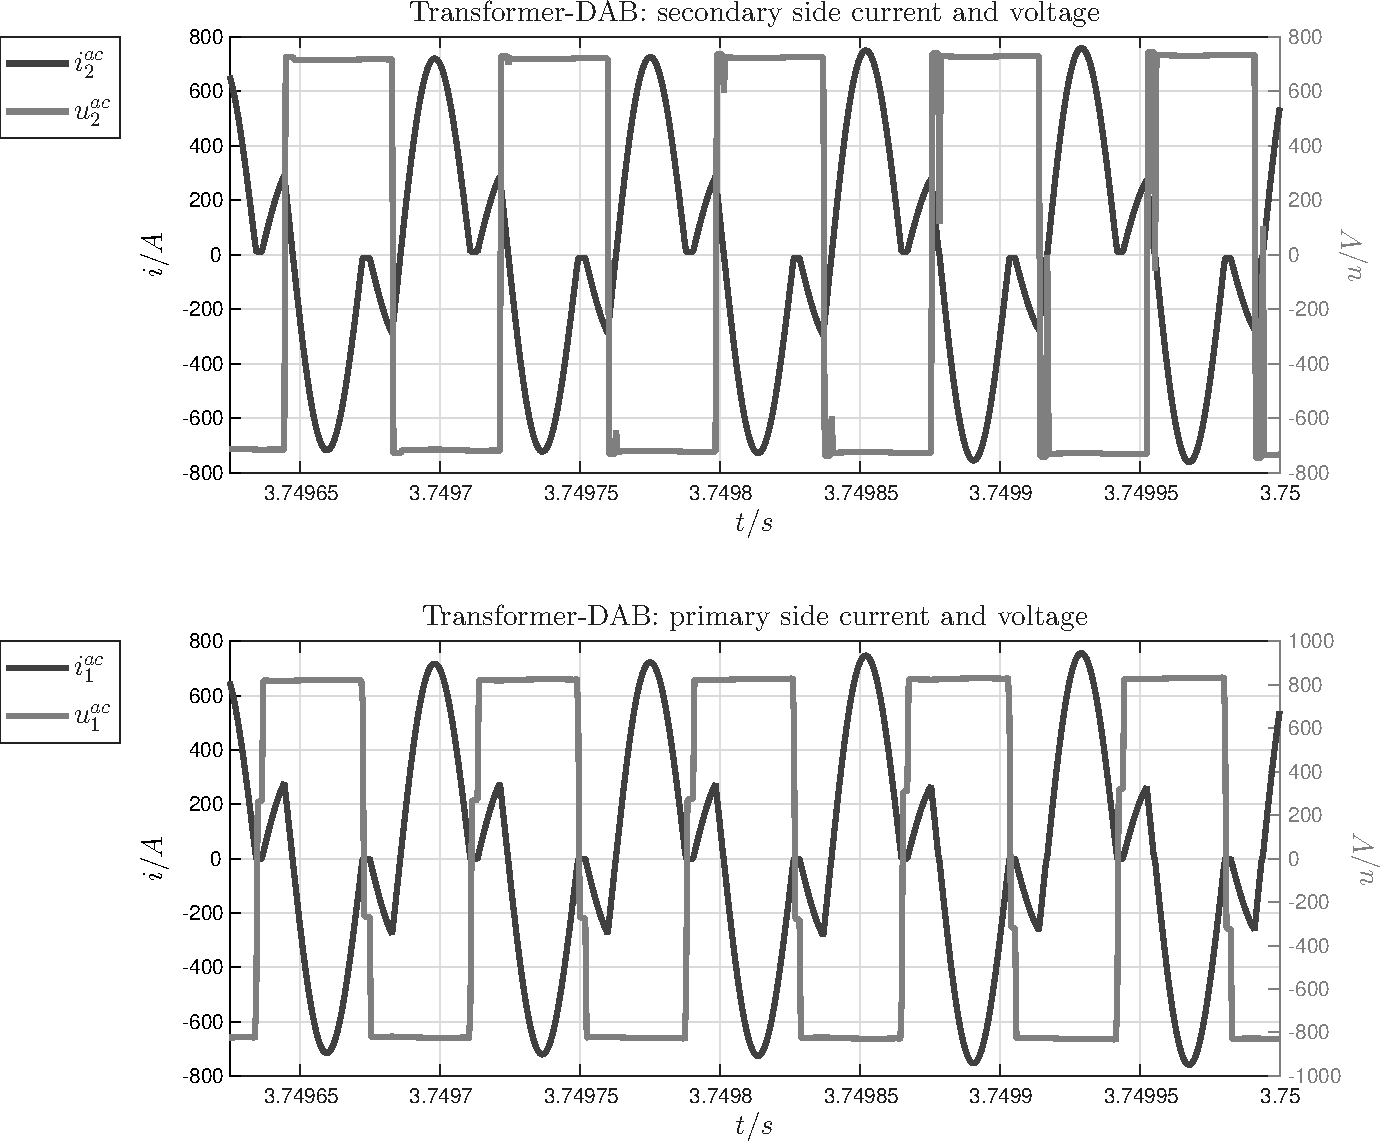
\includegraphics[width =225pt, angle = 0, 
		keepaspectratio]{figures/sim_results/single_phase_llc/dab_transformer_voltage_current}
		\captionsetup{width=0.75\textwidth, font=footnotesize}	
		\caption{Single phase CLLC operative condition at nominal flow power.}
		\label{}
	\end{subfigure}
	\captionsetup{width=0.65\textwidth, font=small}	
	\caption{Single phase CLLC with NPC single phase inverter - single phase inverter and single phase CLLC performances.}
	\label{}
\end{figure}

\begin{figure}[H]
	\centering
	\begin{subfigure}{0.5\textwidth}
		\centering
		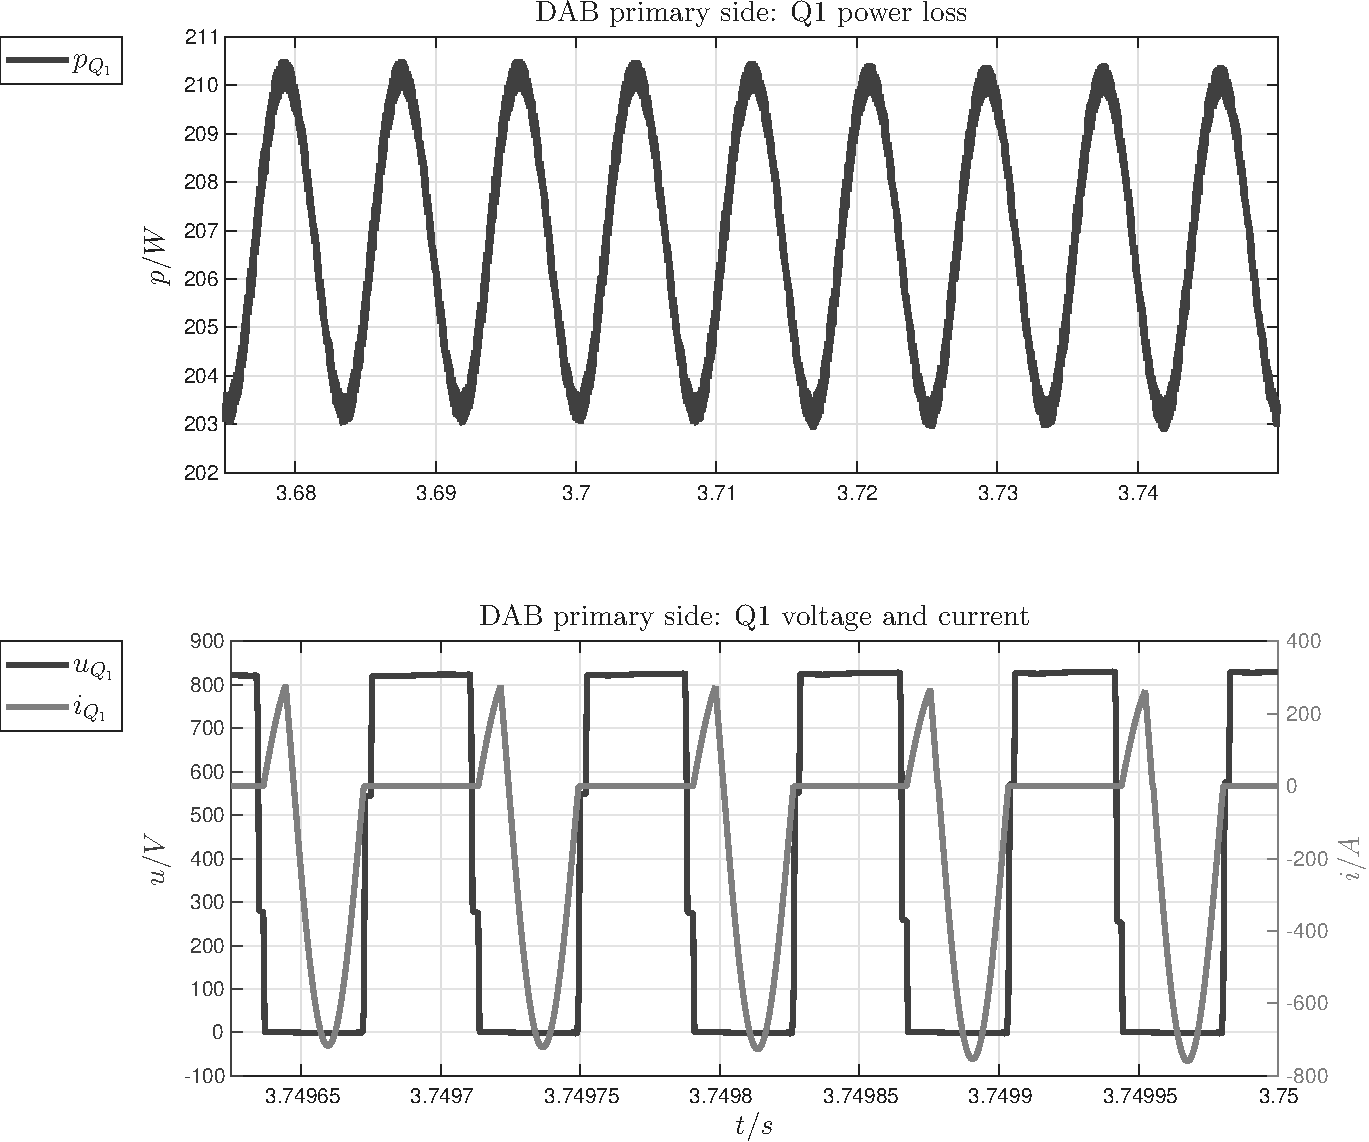
\includegraphics[width =225pt, angle = 0, 
		keepaspectratio]{figures/sim_results/single_phase_llc/DAB_primary_side_Q1}
		\captionsetup{width=0.95\textwidth, font=footnotesize}	
		\caption{Single phase CLLC - primary inverter: Q1-MOSFET power loss, voltage and current.}
		\label{}
	\end{subfigure}%
	\begin{subfigure}{0.5\textwidth}
		\centering
		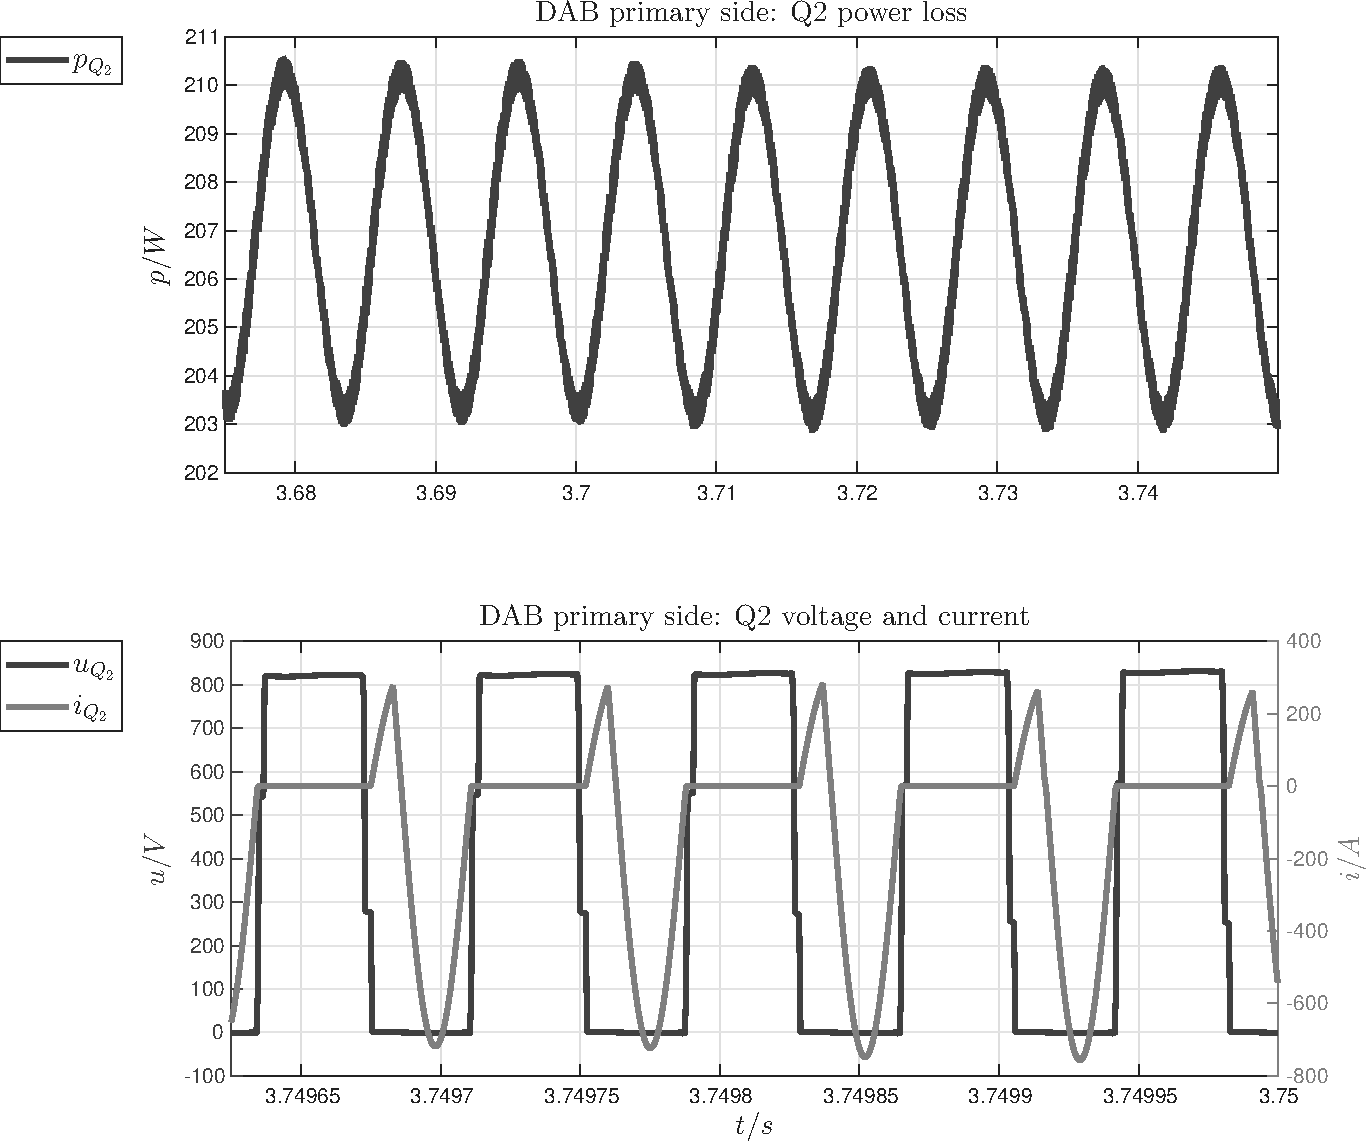
\includegraphics[width =225pt, angle = 0, 
		keepaspectratio]{figures/sim_results/single_phase_llc/DAB_primary_side_Q2}
		\captionsetup{width=0.75\textwidth, font=footnotesize}	
		\caption{Single phase CLLC - primary inverter: Q2-MOSFET power loss, voltage and current.}
		\label{}
	\end{subfigure}
	\captionsetup{width=0.65\textwidth, font=small}	
	\caption{Single phase CLLC with NPC single phase inverter - primary inverter devices performances.}
	\label{}
\end{figure}


\begin{figure}[H]
	\centering
	\begin{subfigure}{0.5\textwidth}
		\centering
		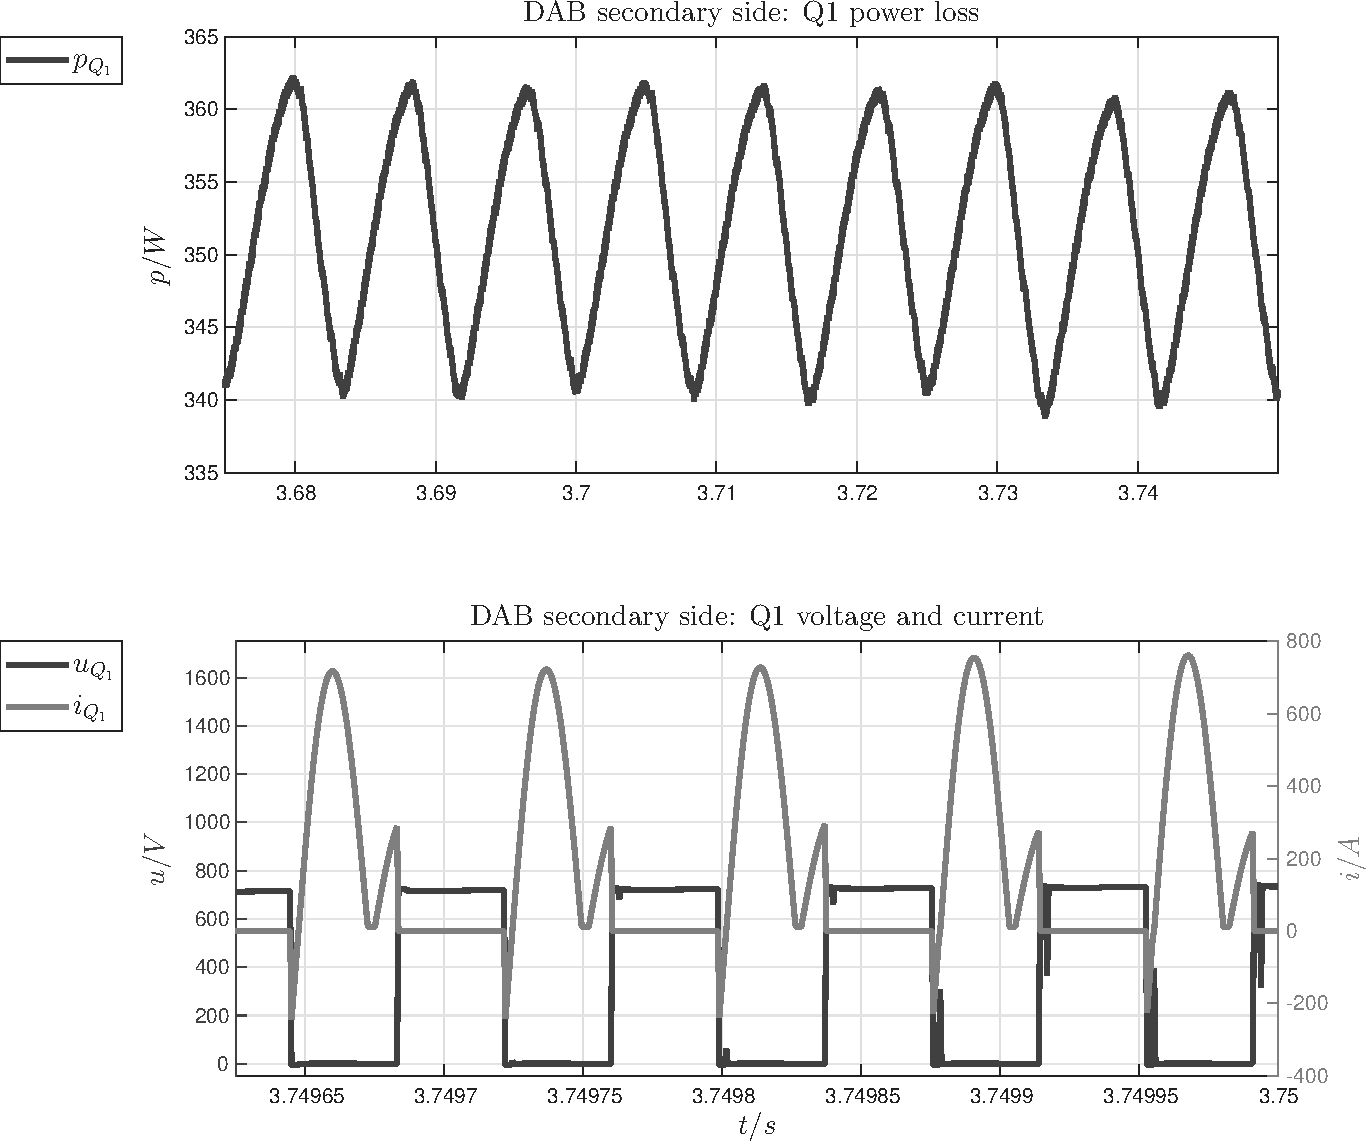
\includegraphics[width =225pt, angle = 0, 
		keepaspectratio]{figures/sim_results/single_phase_llc/DAB_secondary_side_Q1}
		\captionsetup{width=0.95\textwidth, font=footnotesize}	
		\caption{Single phase CLLC - secondary inverter: Q1-MOSFET power loss, voltage and current.}
		\label{}
	\end{subfigure}%
	\begin{subfigure}{0.5\textwidth}
		\centering
		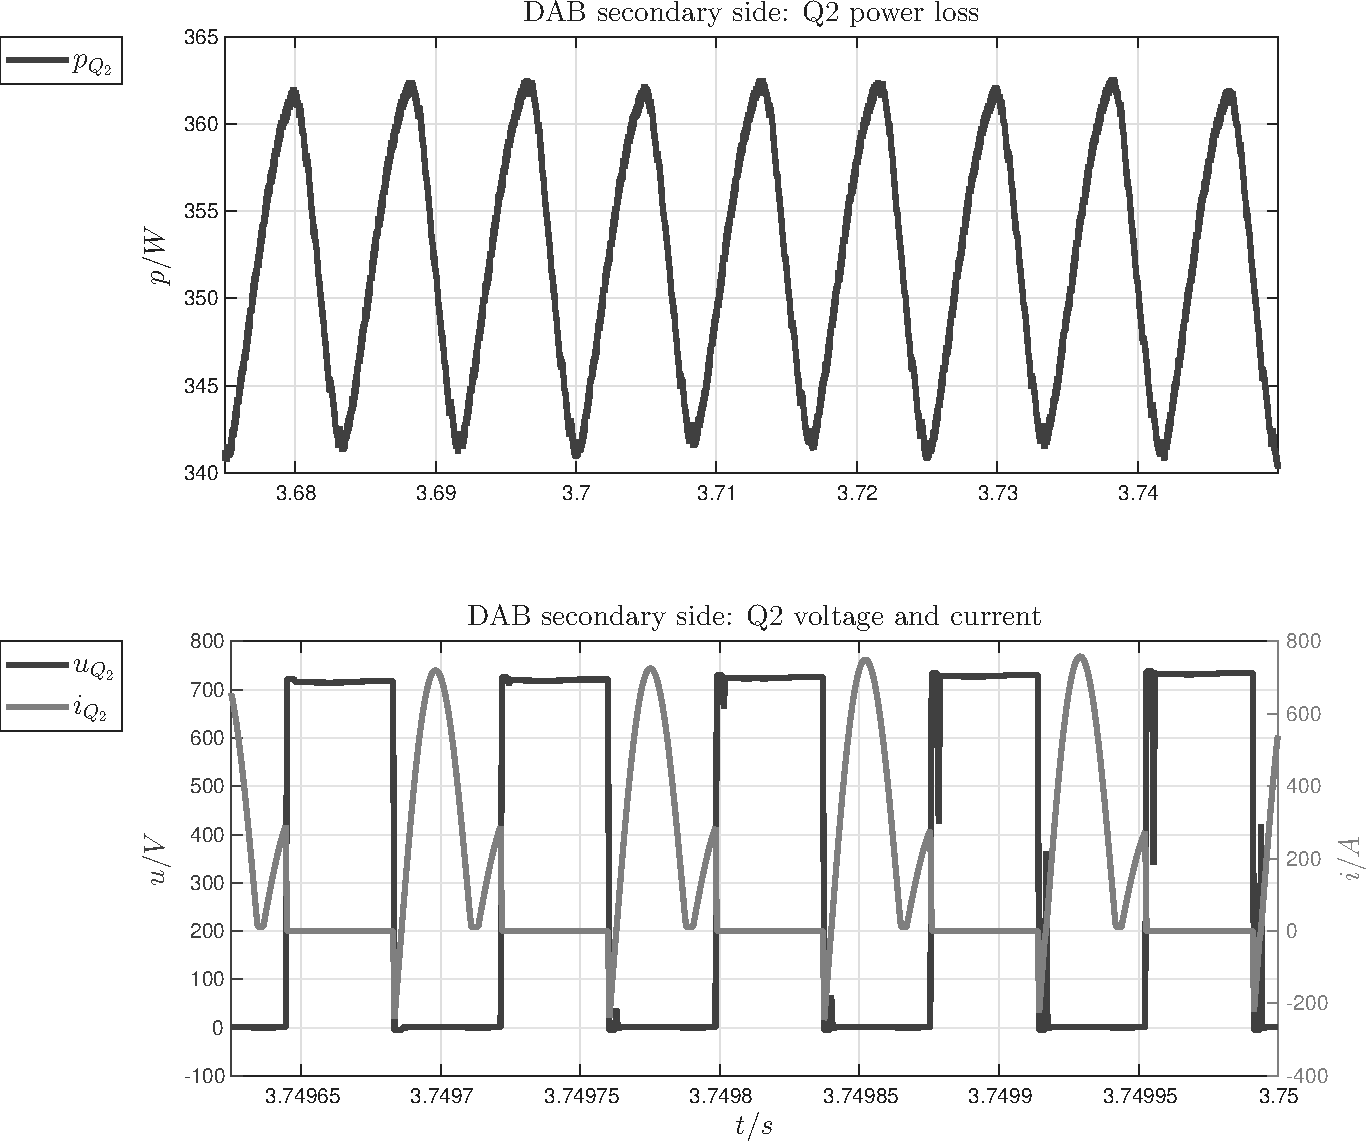
\includegraphics[width =225pt, angle = 0, 
		keepaspectratio]{figures/sim_results/single_phase_llc/DAB_secondary_side_Q2}
		\captionsetup{width=0.75\textwidth, font=footnotesize}	
		\caption{Single phase CLLC - secondary inverter: Q2-MOSFET power loss, voltage and current.}
		\label{}
	\end{subfigure}
	\captionsetup{width=0.65\textwidth, font=small}	
	\caption{Single phase CLLC with NPC single phase inverter - secondary inverter devices performances.}
	\label{}
\end{figure}

\subsection{SST based on Single Phase DAB and NPC Single Phase Inverter}

Single phase DAB performance.

\begin{figure}[H]
	\centering
	\begin{subfigure}{0.5\textwidth}
		\centering
		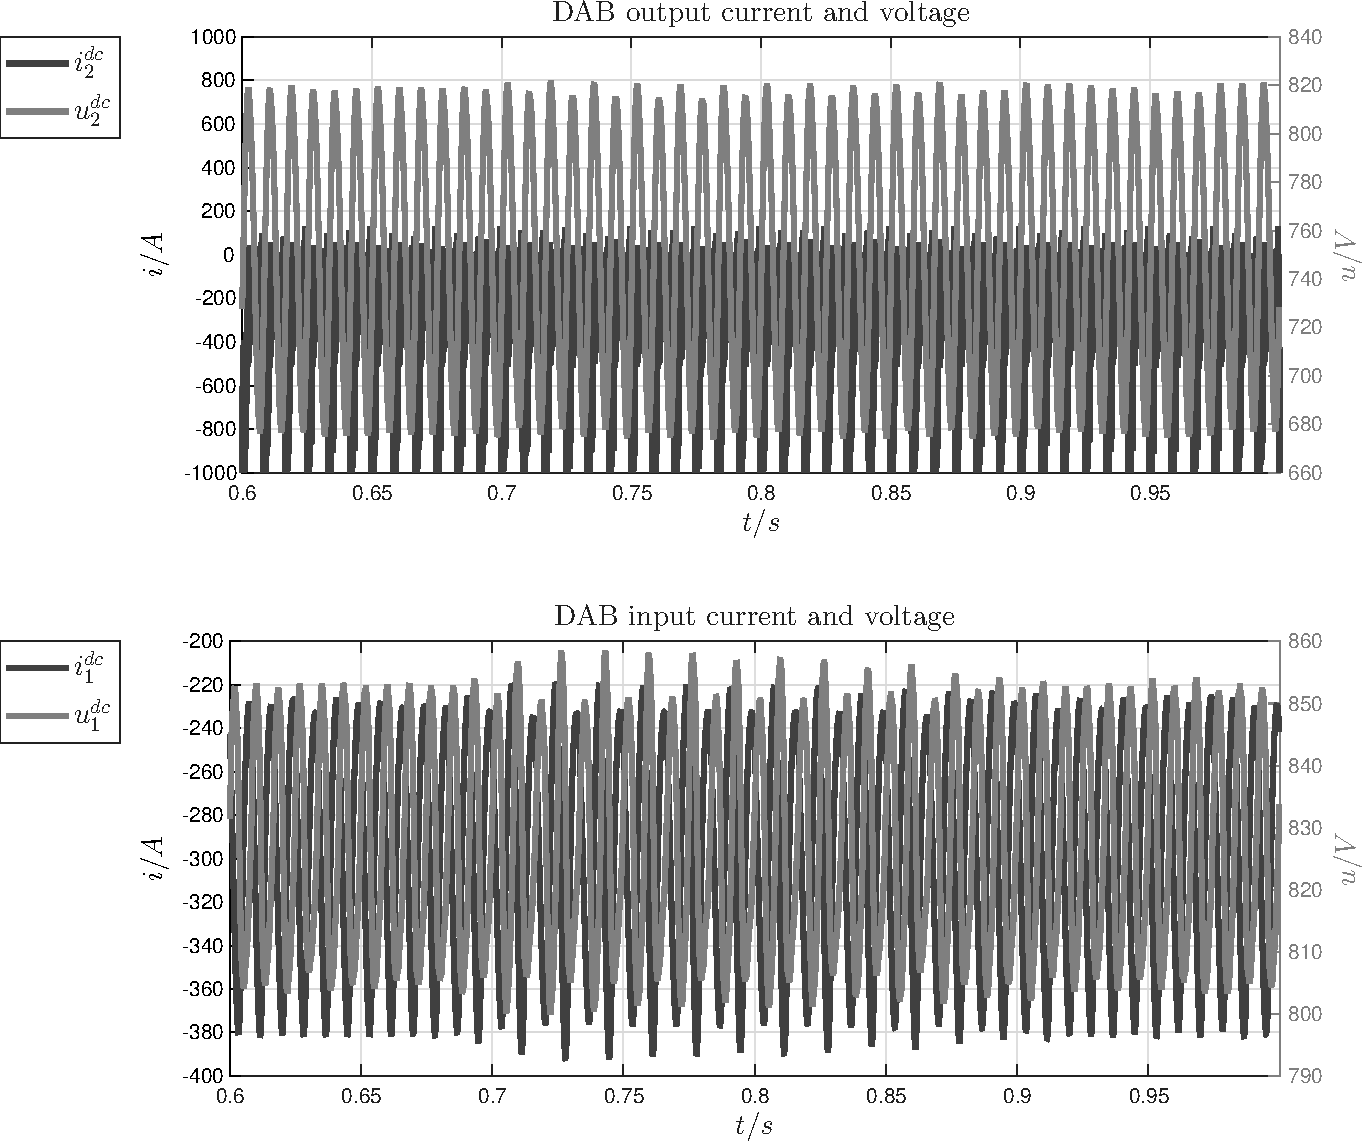
\includegraphics[width =225pt, angle = 0, 
		keepaspectratio]{figures/sim_results/single_phase_dab/dab_ui_output_input}
		\captionsetup{width=0.95\textwidth, font=footnotesize}	
		\caption{Master single phase DAB input current and voltage (bottom) and outputs (top).}
		\label{}
	\end{subfigure}%
	\begin{subfigure}{0.5\textwidth}
		\centering
		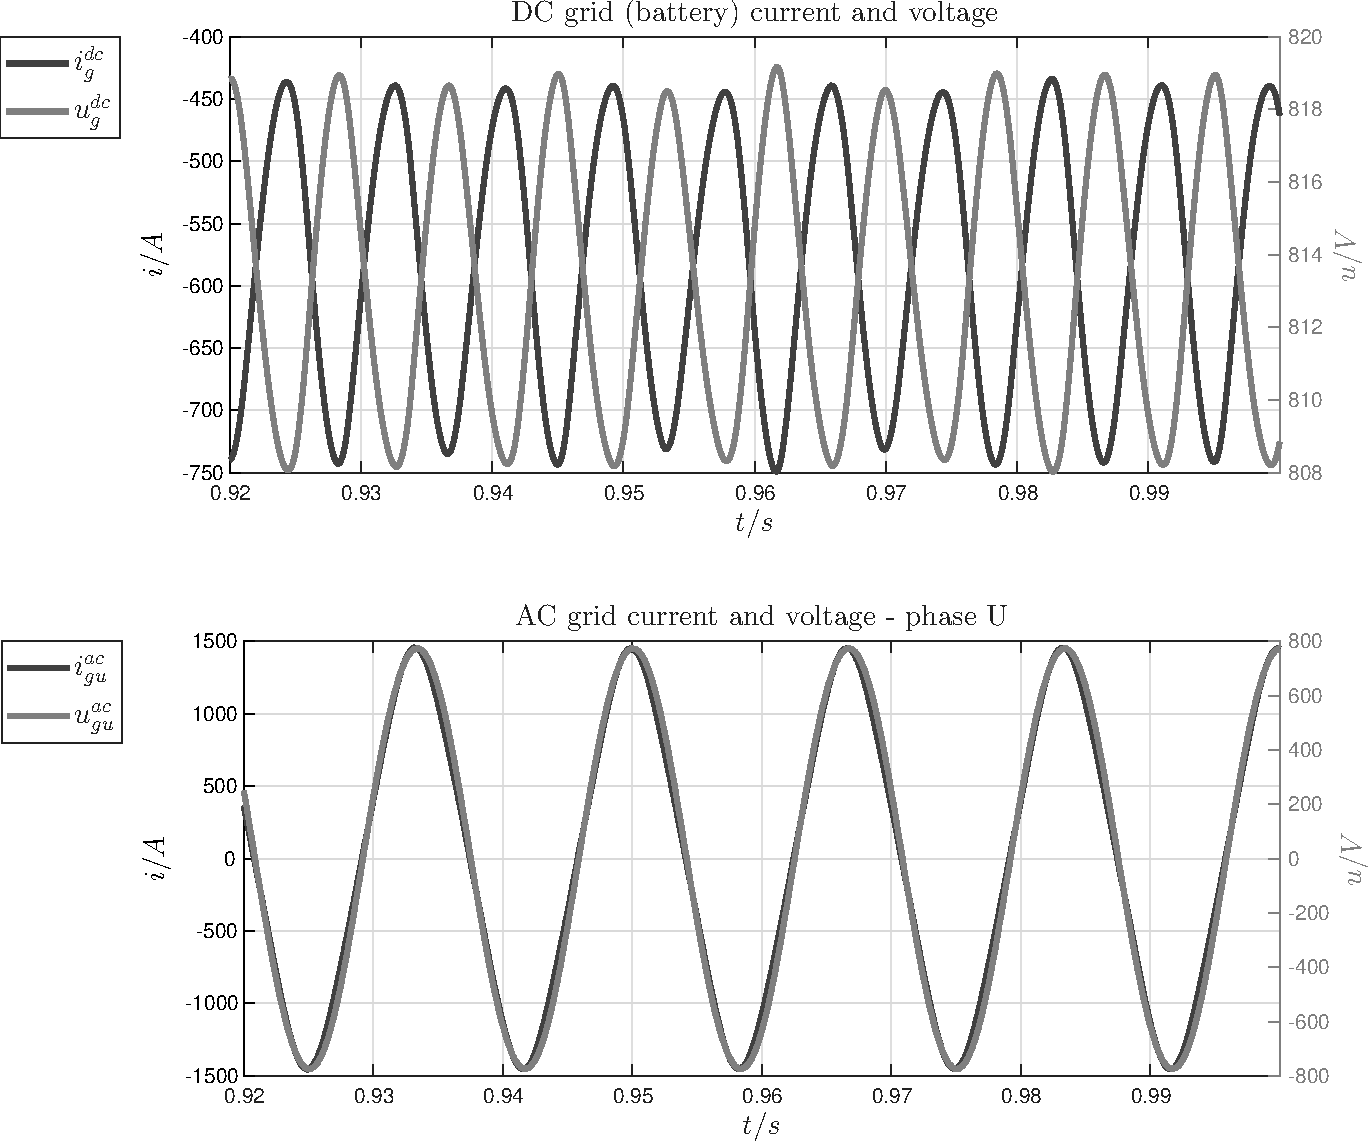
\includegraphics[width =225pt, angle = 0, 
		keepaspectratio]{figures/sim_results/single_phase_dab/dc_ac_grid_voltage_current}
		\captionsetup{width=0.75\textwidth, font=footnotesize}	
		\caption{DC grid current and voltage (top) and AC grid current and voltage (bottom).}	
		\label{}
	\end{subfigure}
	\captionsetup{width=0.65\textwidth, font=small}	
	\caption{Single phase DAB with NPC single phase inverter - performance of two stages single phase SST: single phase DAB input/output and grids.}
	\label{}
\end{figure}

\begin{figure}[H]
	\centering
	\begin{subfigure}{0.5\textwidth}
		\centering
		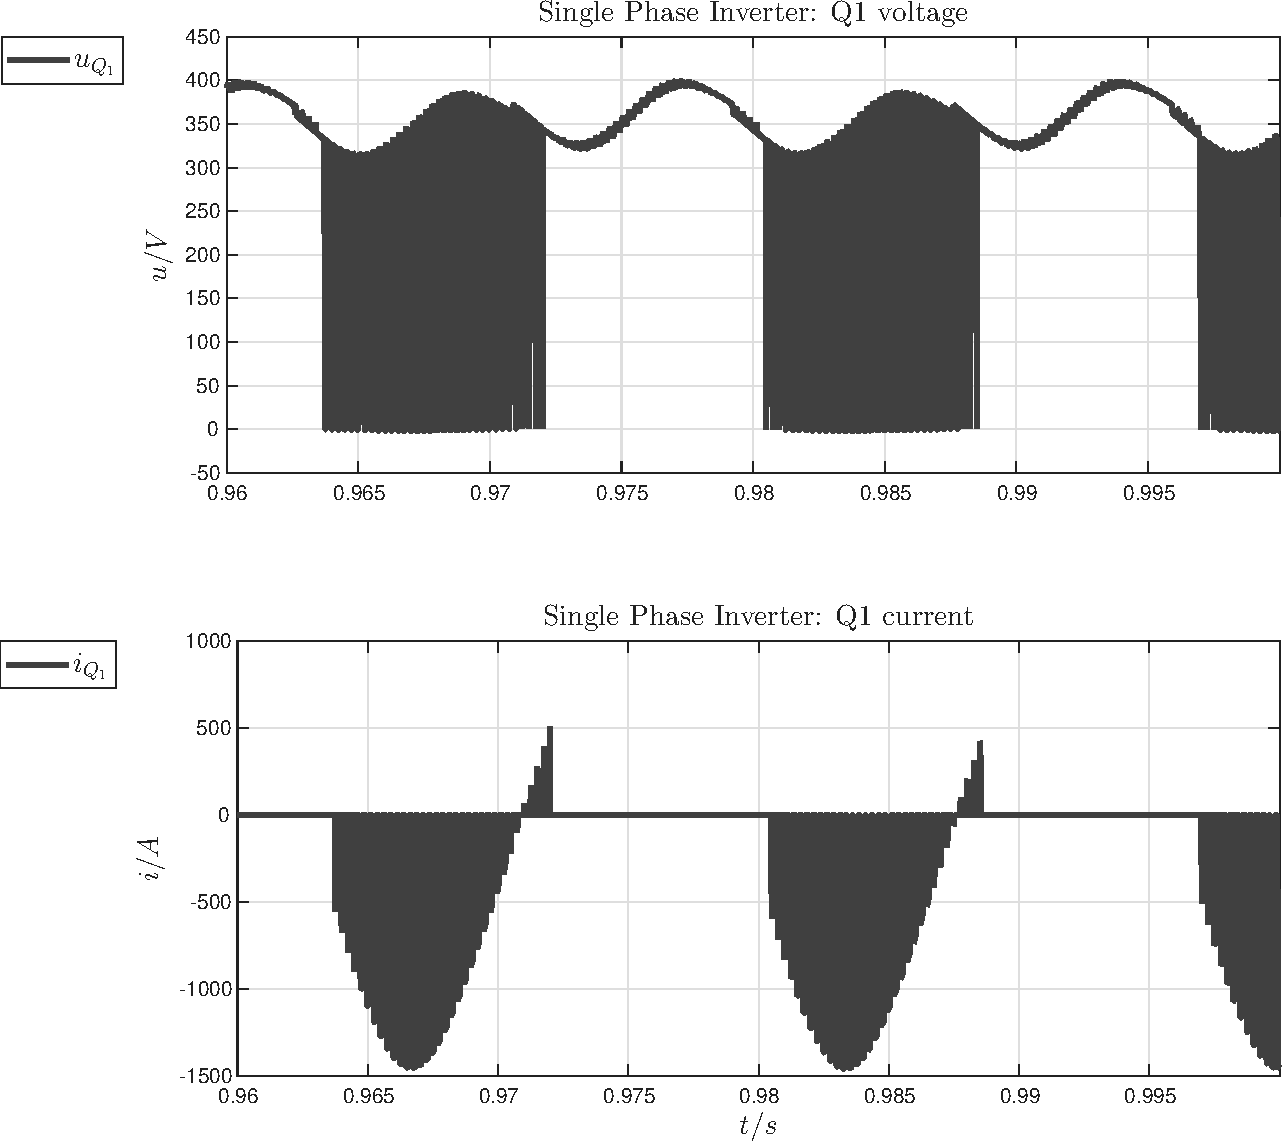
\includegraphics[width =225pt, angle = 0, 
		keepaspectratio]{figures/sim_results/single_phase_dab/single_phase_inverter_Q1}
		\captionsetup{width=0.95\textwidth, font=footnotesize}	
		\caption{Single phase inverter: Q1-IGBT voltage and current. The aim of this image is to proof the effective operative working of the three level NPC single phase inverter.}
		\label{}
	\end{subfigure}%
	\begin{subfigure}{0.5\textwidth}
		\centering
		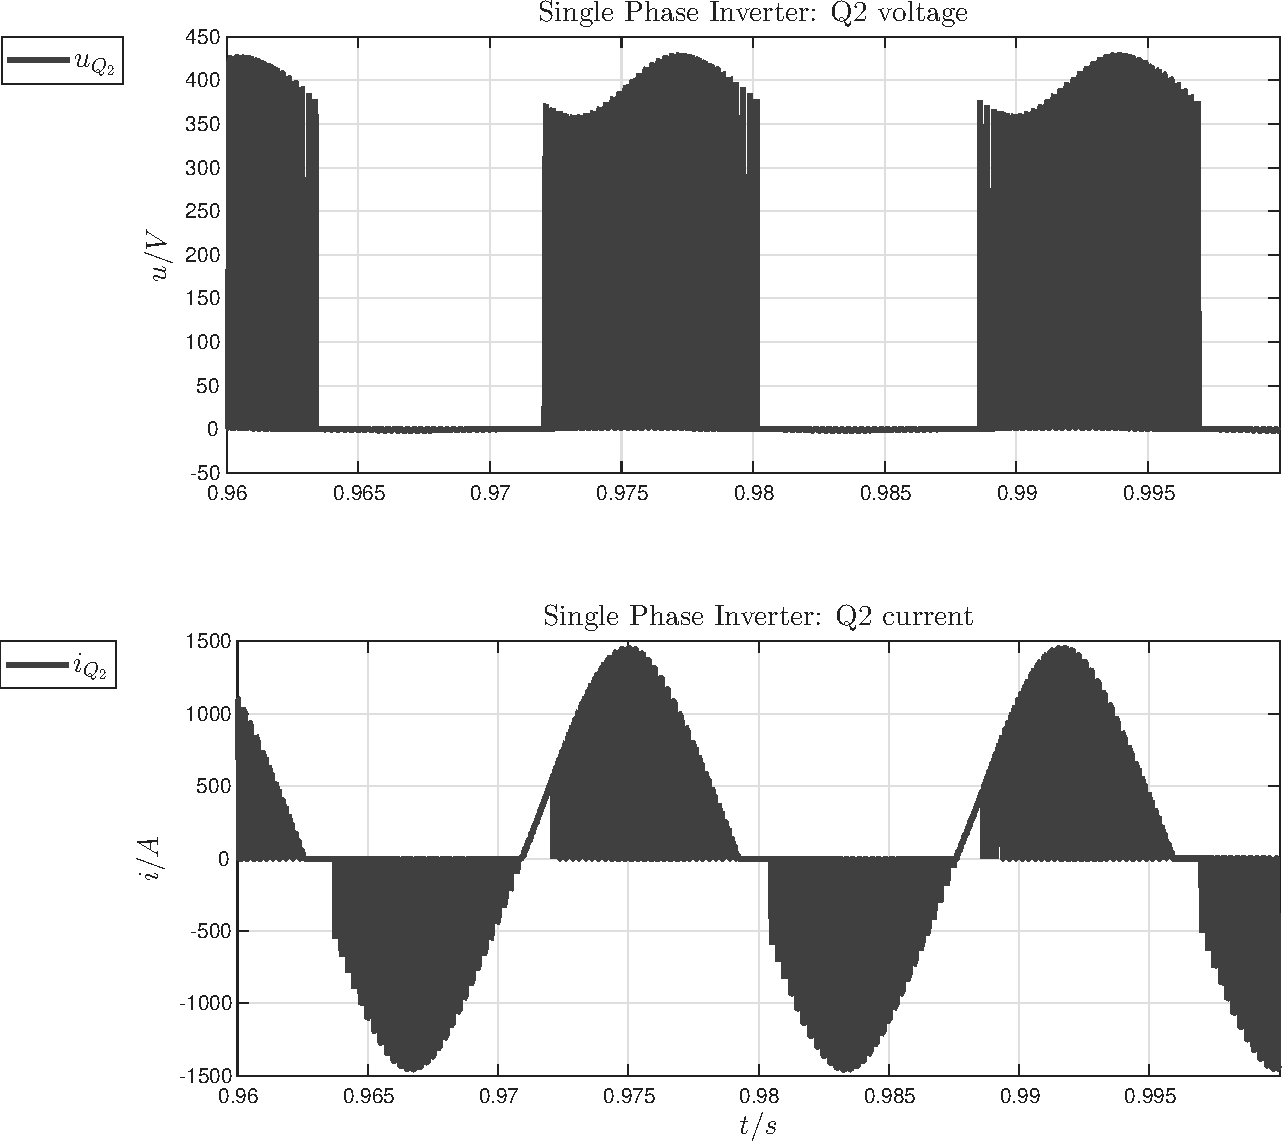
\includegraphics[width =225pt, angle = 0, 
		keepaspectratio]{figures/sim_results/single_phase_dab/single_phase_inverter_Q2}
		\captionsetup{width=0.75\textwidth, font=footnotesize}	
		\caption{Single phase inverter: Q2-IGBT voltage and current. The aim of this image is to proof the effective operative working of the three level NPC single phase inverter.}
		\label{}
	\end{subfigure}
	\captionsetup{width=0.65\textwidth, font=small}	
	\caption{Single phase DAB with NPC single phase inverter - single phase inverter NPC: IGBTs voltage and current.}
	\label{}
\end{figure}


\begin{figure}[H]
	\centering
	\begin{subfigure}{0.5\textwidth}
		\centering
		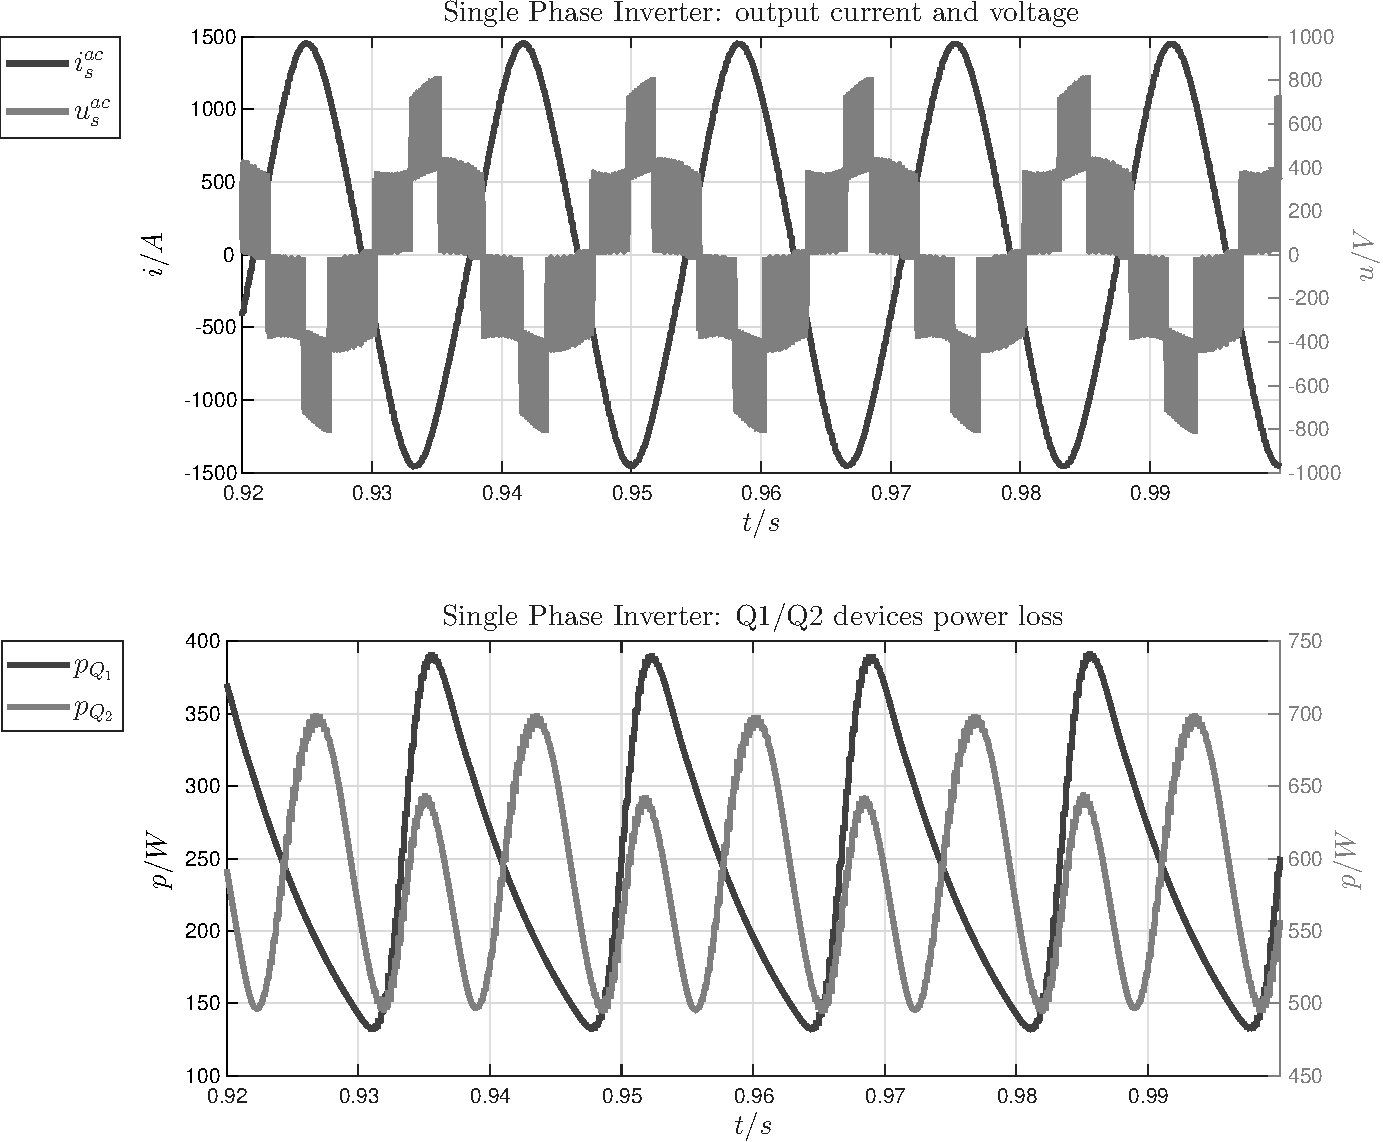
\includegraphics[width =225pt, angle = 0, 
		keepaspectratio]{figures/sim_results/single_phase_dab/single_phase_inverter_performance}
		\captionsetup{width=0.95\textwidth, font=footnotesize}	
		\caption{IGBT Q1 and Q2 power loss (bottom). Single phase output current and voltage, before the output filter (top).}
		\label{}
	\end{subfigure}%
	\begin{subfigure}{0.5\textwidth}
		\centering
		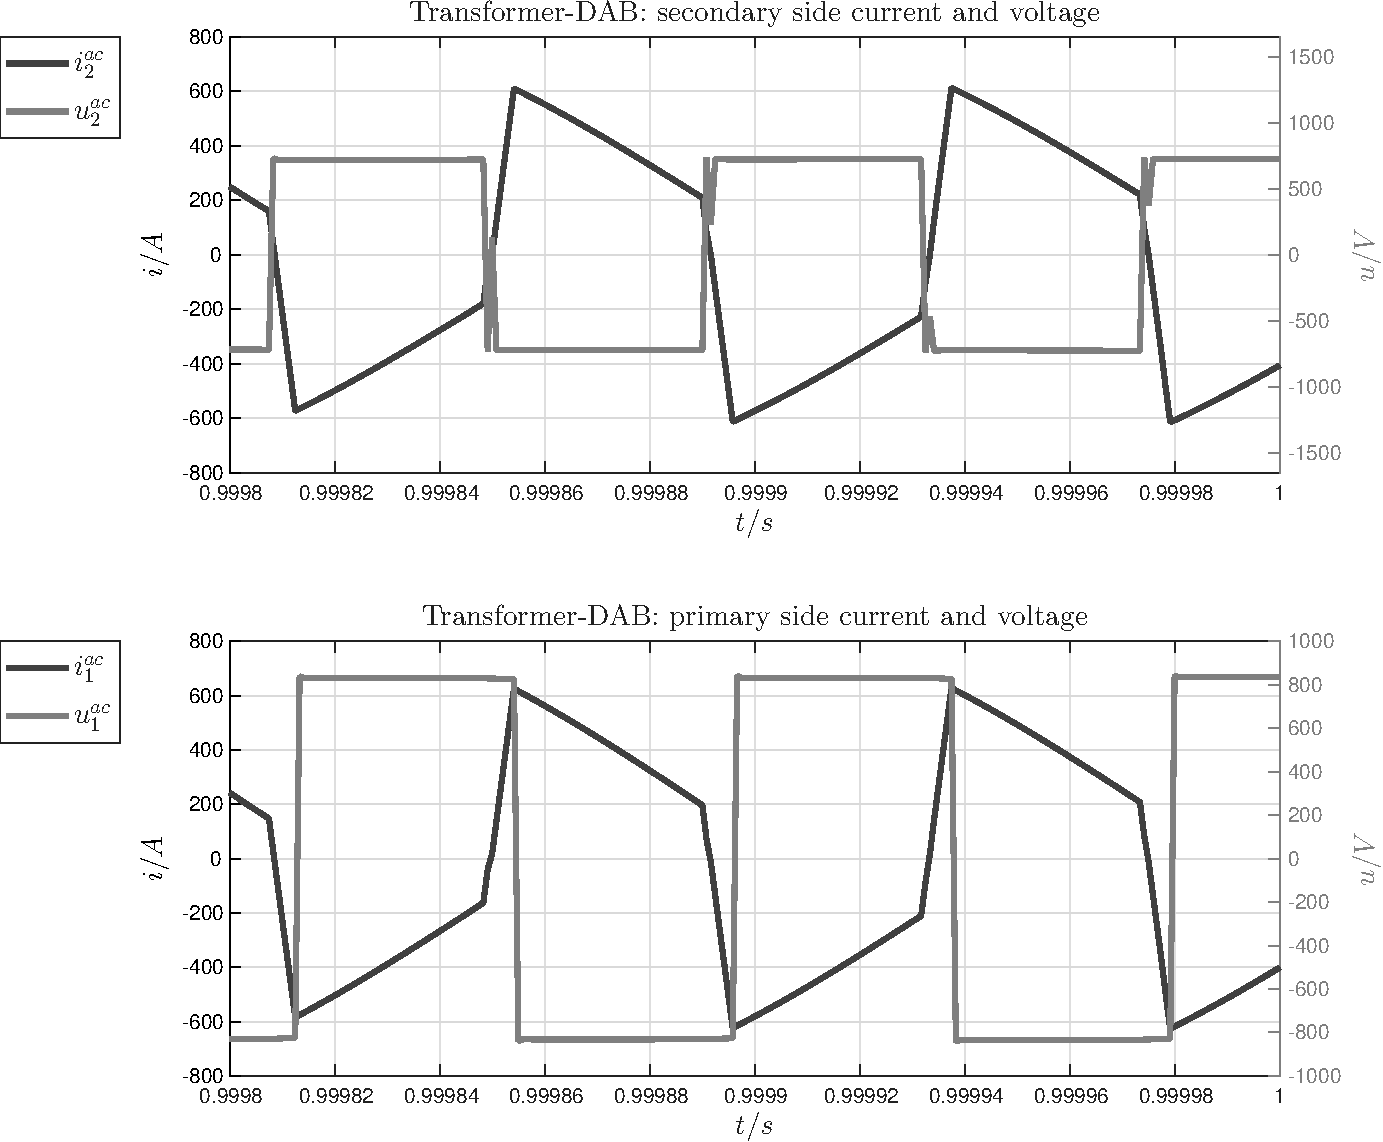
\includegraphics[width =225pt, angle = 0, 
		keepaspectratio]{figures/sim_results/single_phase_dab/dab_transformer_voltage_current}
		\captionsetup{width=0.75\textwidth, font=footnotesize}	
		\caption{Single phase DAB operative condition at nominal flow power.}
		\label{}
	\end{subfigure}
	\captionsetup{width=0.65\textwidth, font=small}	
	\caption{Single phase DAB with NPC single phase inverter - single phase inverter and single phase DAB performances.}
	\label{}
\end{figure}


\begin{figure}[H]
	\centering
	\begin{subfigure}{0.5\textwidth}
		\centering
		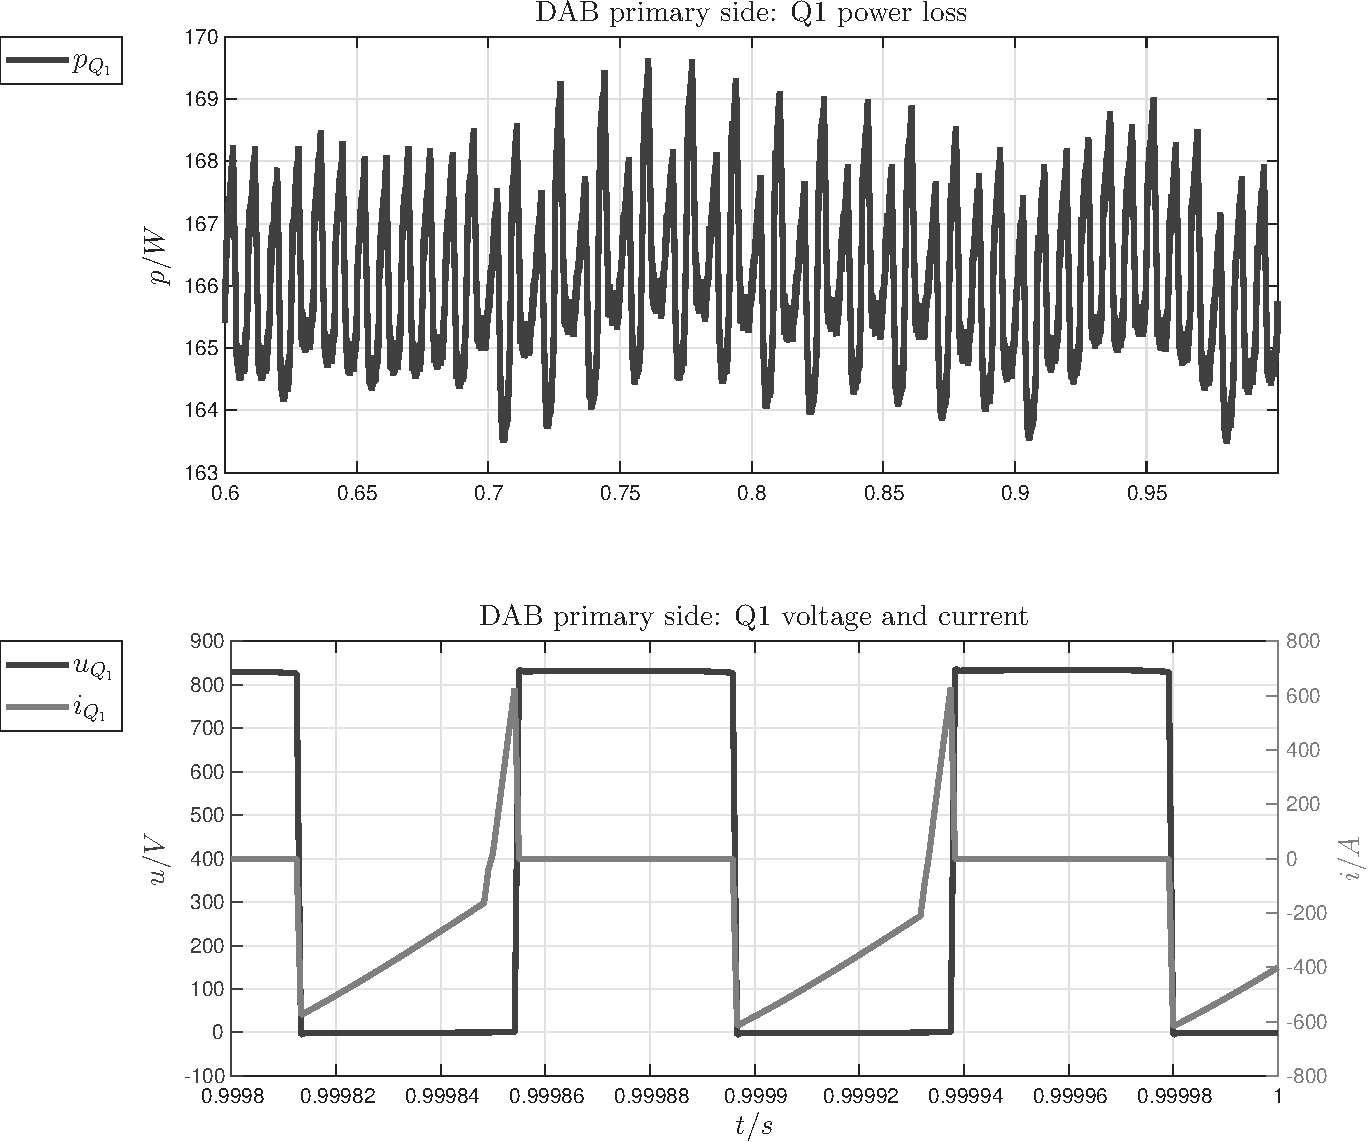
\includegraphics[width =225pt, angle = 0, 
		keepaspectratio]{figures/sim_results/single_phase_dab/DAB_primary_side_Q1}
		\captionsetup{width=0.95\textwidth, font=footnotesize}	
		\caption{Single phase DAB - primary inverter: Q1-MOSFET power loss, voltage and current.}
		\label{}
	\end{subfigure}%
	\begin{subfigure}{0.5\textwidth}
		\centering
		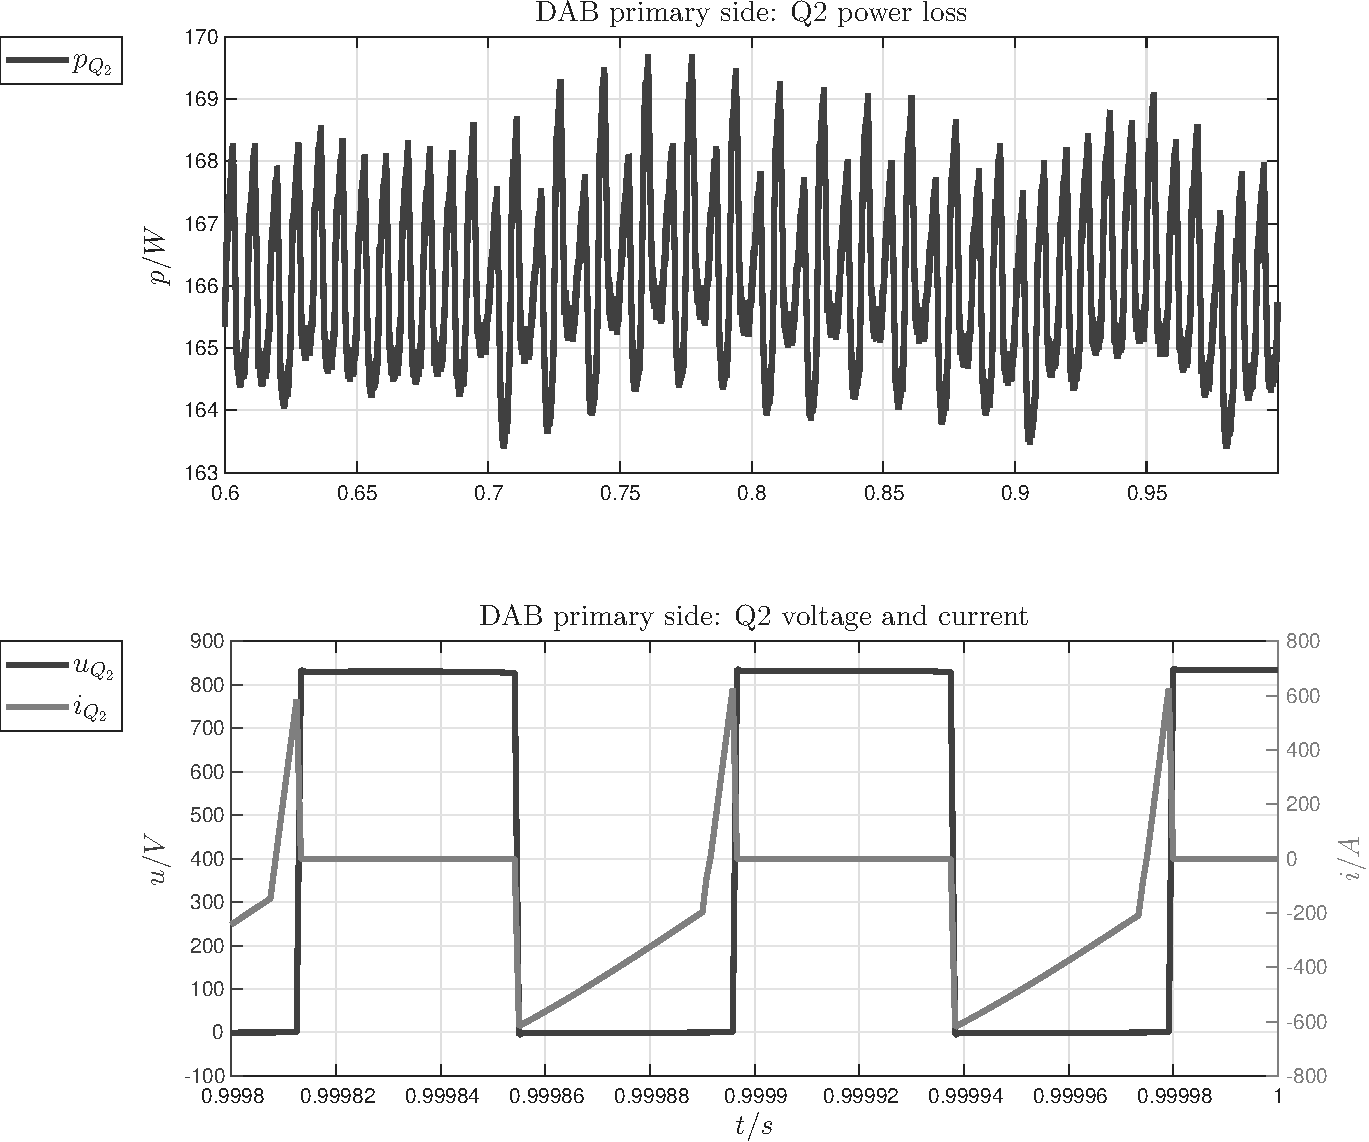
\includegraphics[width =225pt, angle = 0, 
		keepaspectratio]{figures/sim_results/single_phase_dab/DAB_primary_side_Q2}
		\captionsetup{width=0.75\textwidth, font=footnotesize}	
		\caption{Single phase DAB - primary inverter: Q2-MOSFET power loss, voltage and current.}
		\label{}
	\end{subfigure}
	\captionsetup{width=0.65\textwidth, font=small}	
	\caption{Single phase DAB with NPC single phase inverter - primary inverter devices performances.}
	\label{}
\end{figure}

\begin{figure}[H]
	\centering
	\begin{subfigure}{0.5\textwidth}
		\centering
		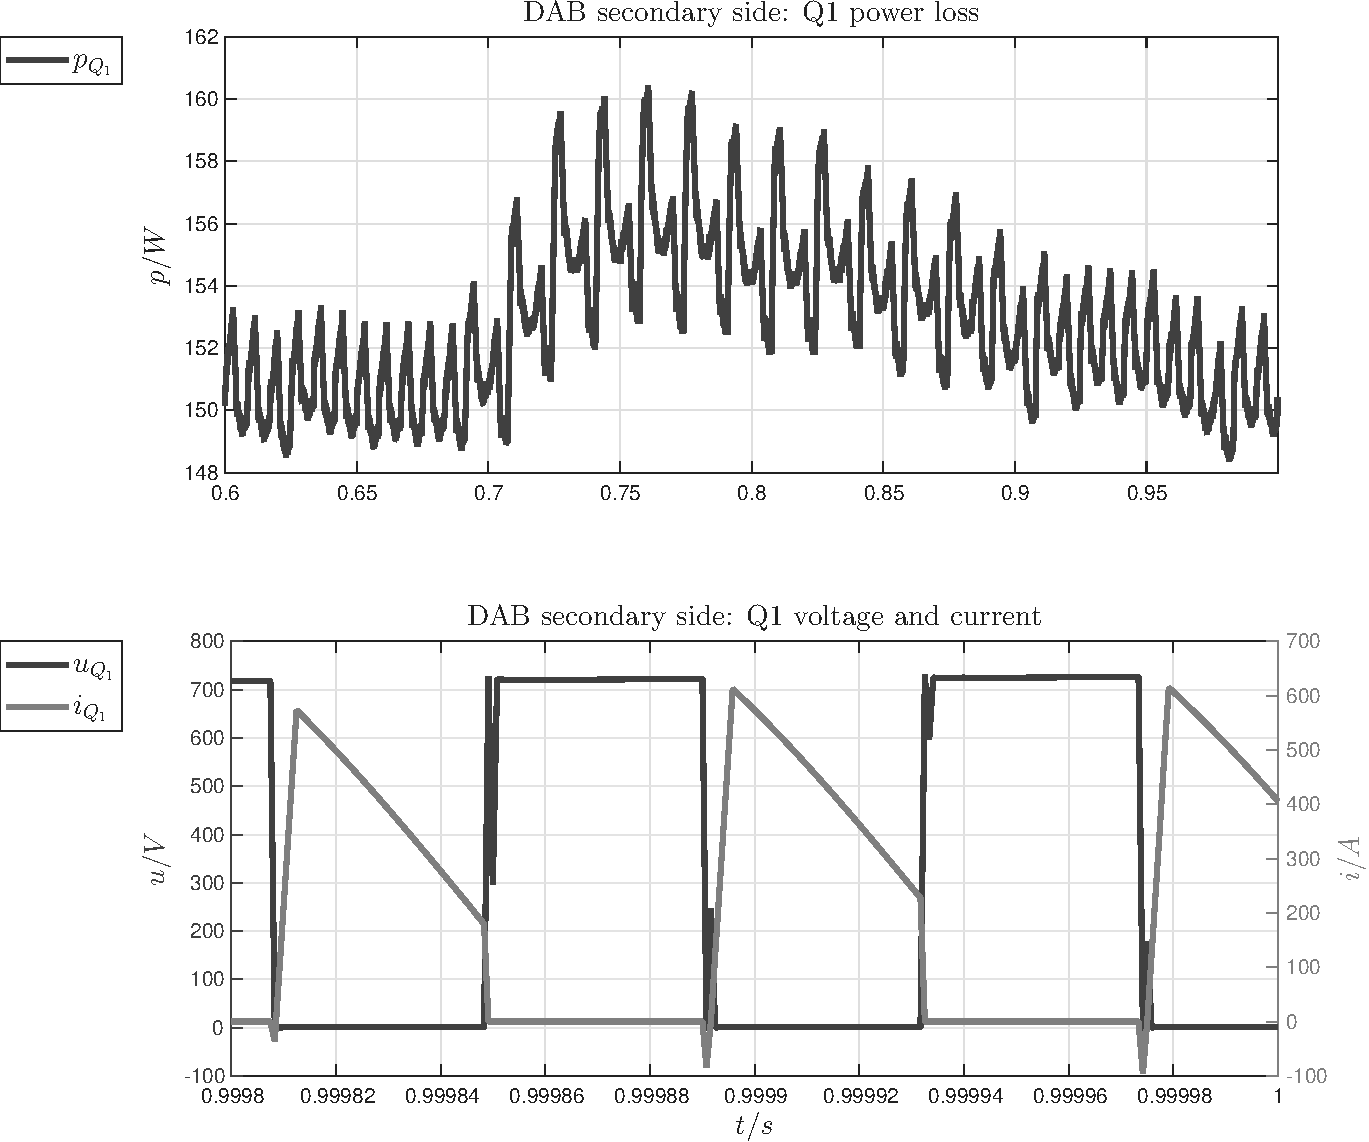
\includegraphics[width =225pt, angle = 0, 
		keepaspectratio]{figures/sim_results/single_phase_dab/DAB_secondary_side_Q1}
		\captionsetup{width=0.95\textwidth, font=footnotesize}	
		\caption{Single phase DAB - secondary inverter: Q1-MOSFET power loss, voltage and current.}
		\label{}
	\end{subfigure}%
	\begin{subfigure}{0.5\textwidth}
		\centering
		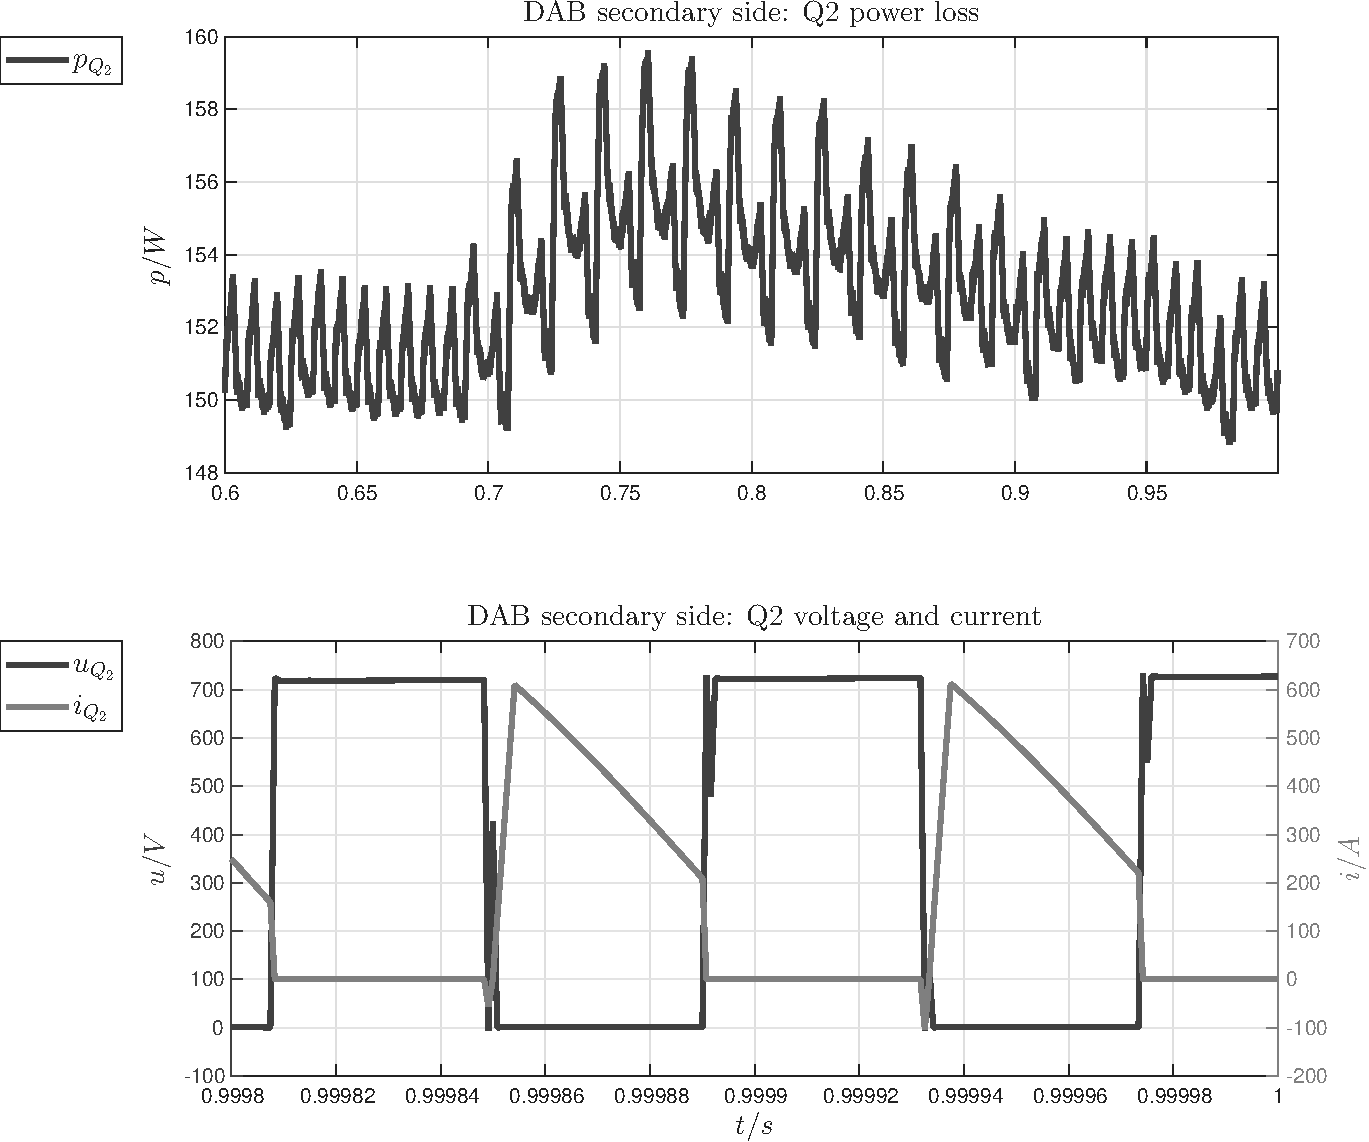
\includegraphics[width =225pt, angle = 0, 
		keepaspectratio]{figures/sim_results/single_phase_dab/DAB_secondary_side_Q2}
		\captionsetup{width=0.75\textwidth, font=footnotesize}	
		\caption{Single phase DAB - secondary inverter: Q2-MOSFET power loss, voltage and current.}
		\label{}
	\end{subfigure}
	\captionsetup{width=0.65\textwidth, font=small}	
	\caption{Single phase DAB with NPC single phase inverter - secondary inverter devices performances.}
	\label{}
\end{figure}

\section{High-Frequency transformers design}

\subsection{Transformer design for 3P-DAB with T-Type single phase inverter architecture}
Transformer for the three-phase DAB is built by three independent single phase transformers, as follows.

\noindent\textbf{Input data}:
\begin{itemize}
	\item[--] $u_1^{b} = \SI{400}{\volt} rms$: primary side nominal voltage;	
	\item[--] $u_2^{b} = \SI{400}{\volt} rms$: secondary side nominal voltage;	
	\item[--] $i_1^{b} = \SI{275}{\ampere} rms$: primary side nominal current;	
	\item[--] $i_2^{b} = \SI{275}{\volt} rms$: secondary side nominal current;
	\item[--] $f_{b} = \SI{4}{\kilo\hertz}$: fundamental frequency;
\end{itemize}

\noindent\textbf{Design}:
\begin{itemize}
	\item[--] core material: nanocrystalline alloy ($\mu_r = \SI{5000}{}$);	
	\item[--] core shape: C (AM-NC-320C AMMET);		
	\begin{itemize}
		\item[--] core height: $h_{fe} = \SI{220}{\milli\meter}$;	
		\item[--] core length: $L_{fe} = \SI{720}{\milli\meter}$;	
		\item[--] core width: $d_{fe} = \SI{50}{\milli\meter}$;		
		\item[--] core window: $W_{fe} = \SI{60}{\milli\meter}$;	
		\item[--] core depth: $D_{fe} = \SI{90}{\milli\meter}$;	
		\item[--] relative permeability $\mu_r = \SI{5000}{}$;
		\item[--] maximum magnetic flux density $\hat{B} = \SI{0.8}{\weber\per\square\meter}$;
	\end{itemize}
	\item[--] winding material: copper foil $d = \SI{0.5}{\milli\meter}$;		
	\item[--] winding current density: $J = \SI{3.0}{\ampere\per\square\milli\meter}$;	
\end{itemize}

\noindent calculus:
assuming $n_1 = n_2 = 6$
\begin{flalign}
	S_{fe} = 10^{4}\frac{u_1^{b}}{4.44\ f_b\ \hat{B}\ n_1} \approx \SI{47}{\square\centi\meter} &&
\end{flalign}
\begin{flalign}
	S_{cu} = \frac{i_1^{b}}{J} \approx \SI{90}{\square\milli\meter} &&
\end{flalign}
\begin{flalign}
	L_{cu} = \frac{S_{cu}}{d} \approx \SI{180}{\milli\meter} &&
\end{flalign}

\noindent\textbf{Remark} - core will be created by the parallelization of 3 per AM-NC-320C AMMET, that results in the following iron power losses: \\


\noindent\textbf{Specific Core Loss} 
\begin{flalign}
	P_{\mu} = \SI{16}{\watt\per\kilogram} \qquad \text{at}\quad f=\SI{4}{\kilo\hertz},\quad \hat{B}=\SI{0.8}{\weber\per\square\meter} &&
\end{flalign}
\noindent\textbf{Core mass}
\begin{flalign}
 m_{fe} = \SI{26.35}{\kilogram}&&
\end{flalign}
\noindent\textbf{Core power losses}
\begin{flalign}
	P_{fe} = \SI{225}{\watt} &&
\end{flalign}
\noindent\textbf{Copper power losses}
\begin{flalign}
	P_{cu} = \SI{50}{\watt} &&
\end{flalign}

\noindent\textbf{Total power losses}
\begin{flalign}
	P_{loss} = 3(P_{fe}+P_{cu}) = \SI{825}{\watt}&&
\end{flalign}

\begin{figure}[H]
	\centering
	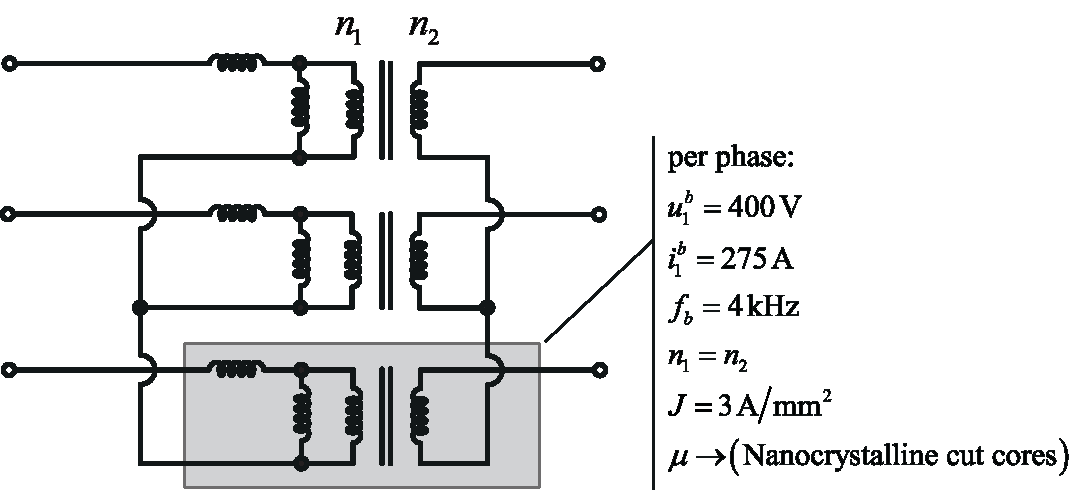
\includegraphics[width = 325pt, angle = 0, 
	keepaspectratio]{figures/magnetics/three_phase_transformers_dab_7}
	\captionsetup{width=0.5\textwidth, font=small}
	\caption{Transformer layout for the three-phase DAB.}
	\label{three_phase_transformers_dab_7}
\end{figure}

\begin{figure}[H]
	\centering
	\begin{subfigure}{0.5\textwidth}
		\centering
		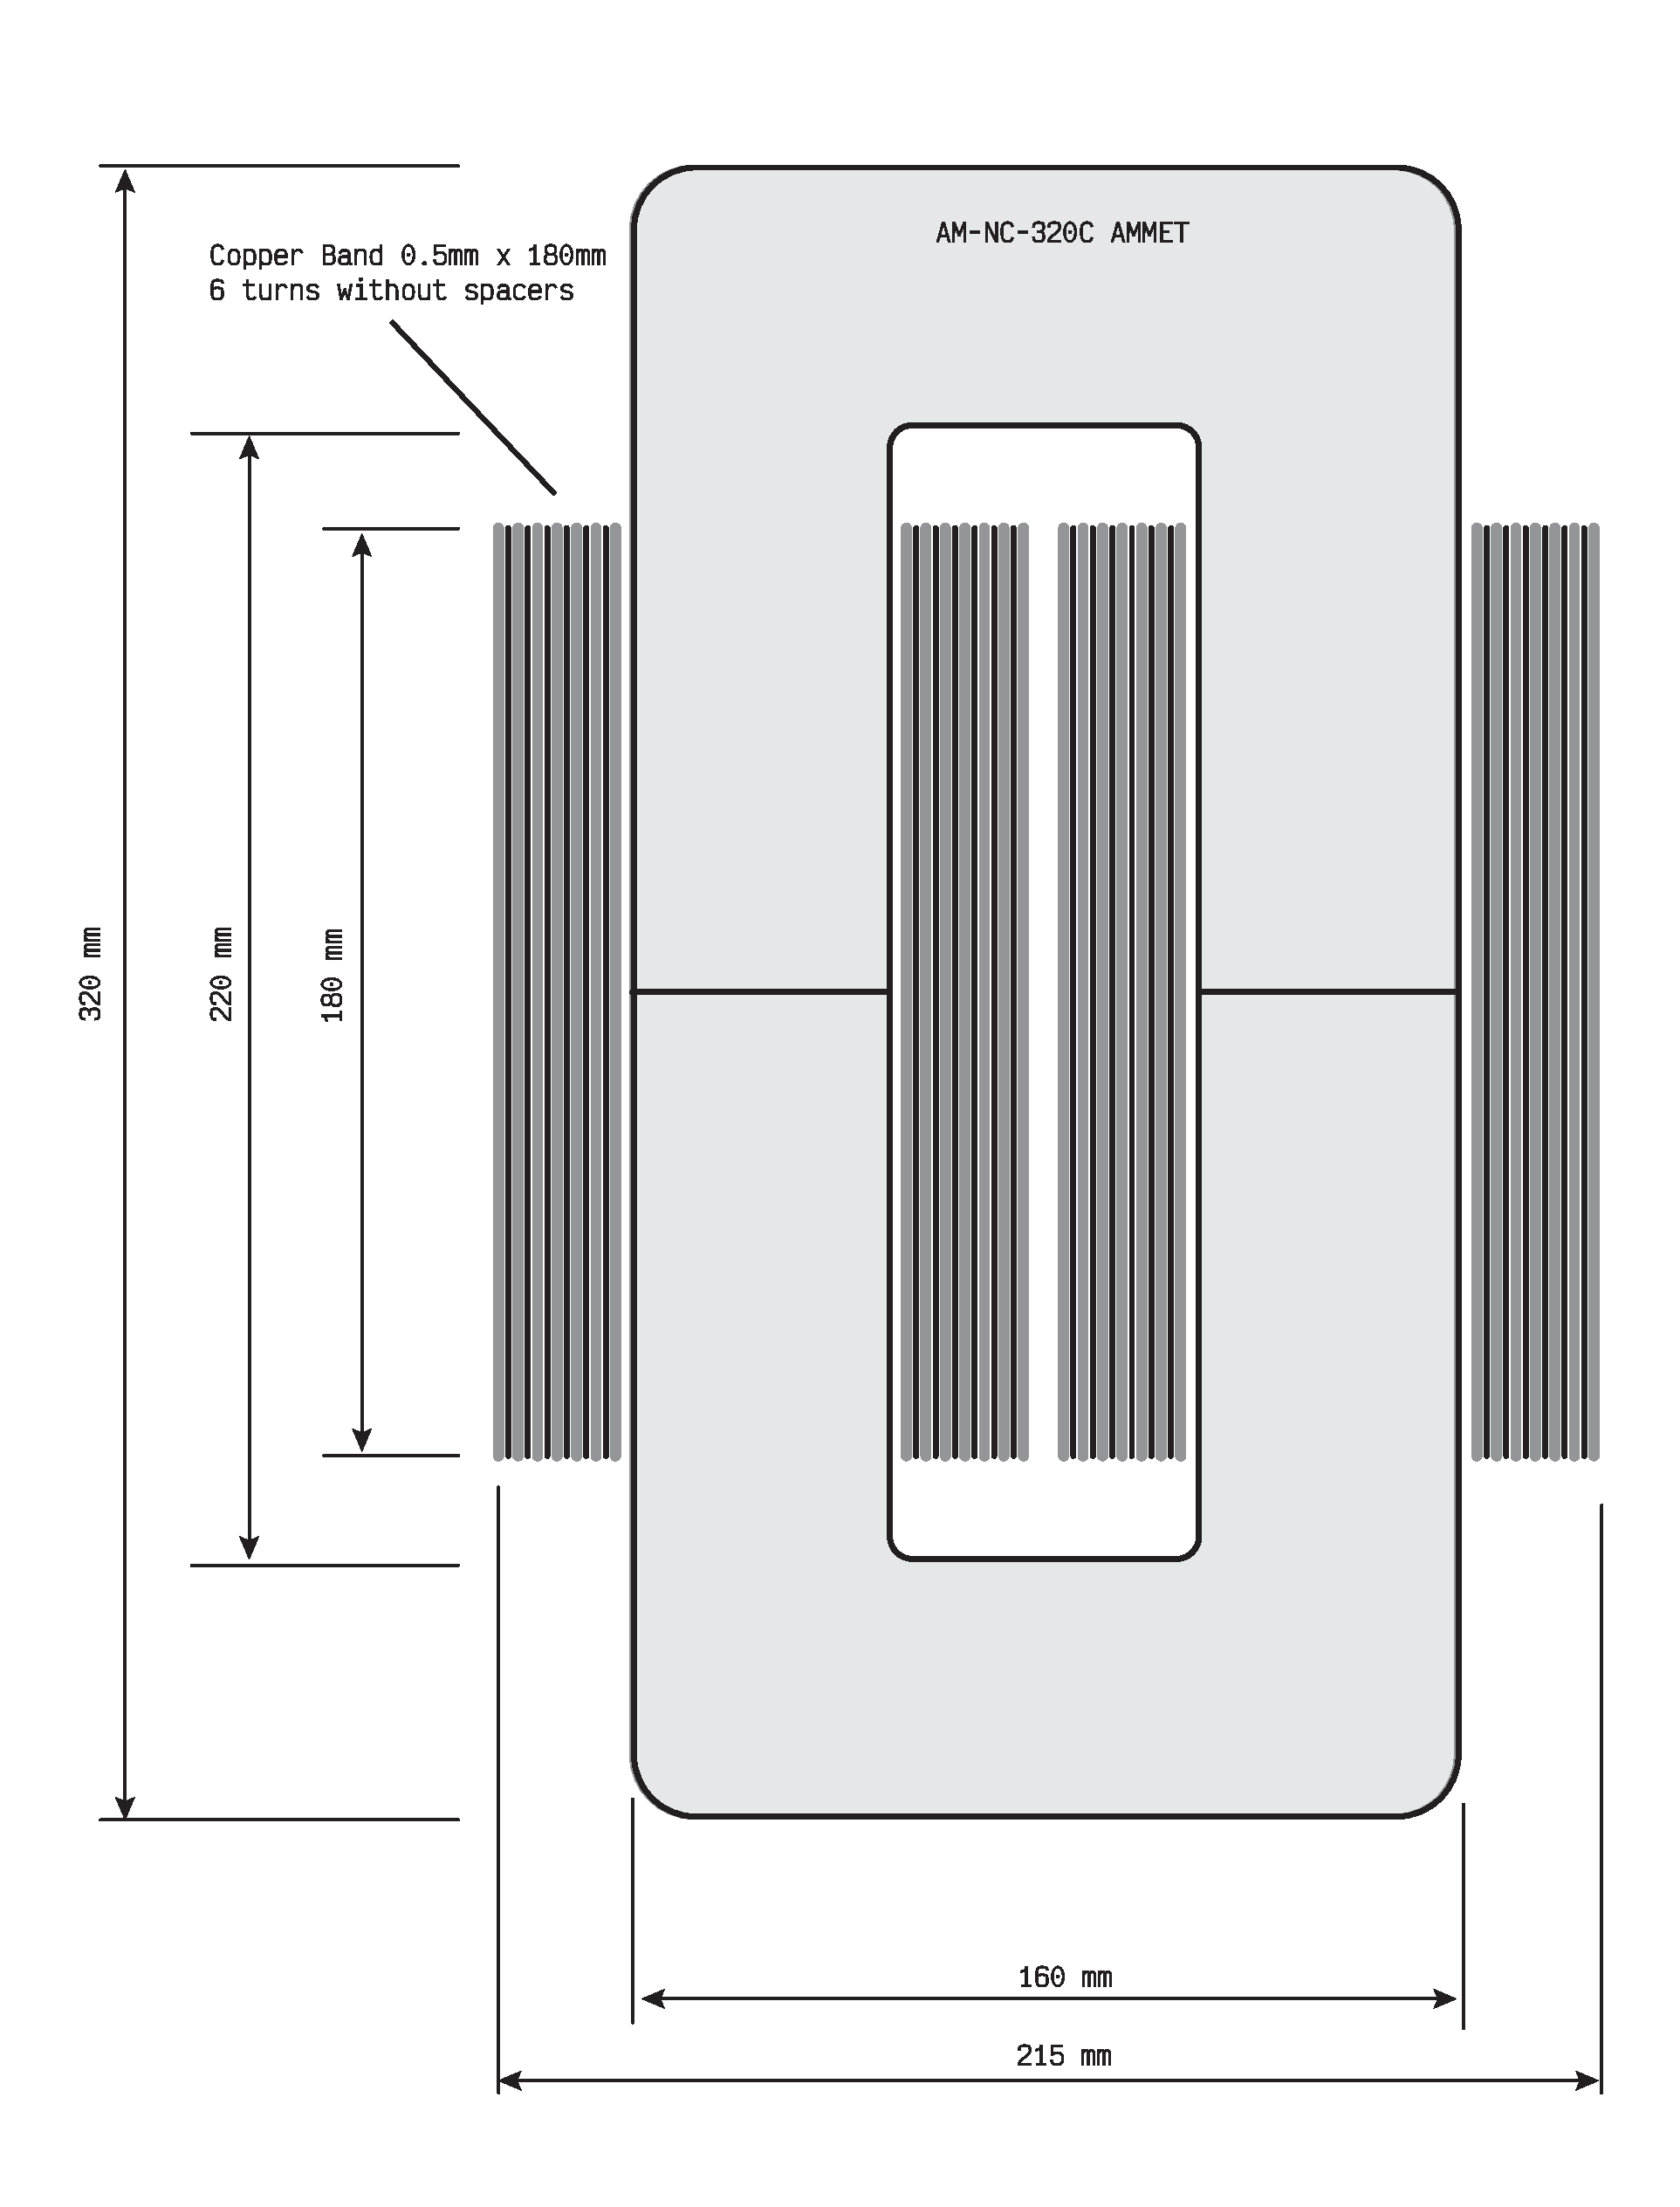
\includegraphics[width =250pt, angle = 0, 
		keepaspectratio]{figures/magnetics/three_phase_transformers_dab_5}
		\captionsetup{width=0.75\textwidth, font=footnotesize}	
		\caption{Single phase transformer for the three-phase DAB - front view.}
		\label{three_phase_transformers_dab_5}
	\end{subfigure}%
	\begin{subfigure}{0.5\textwidth}
		\centering
		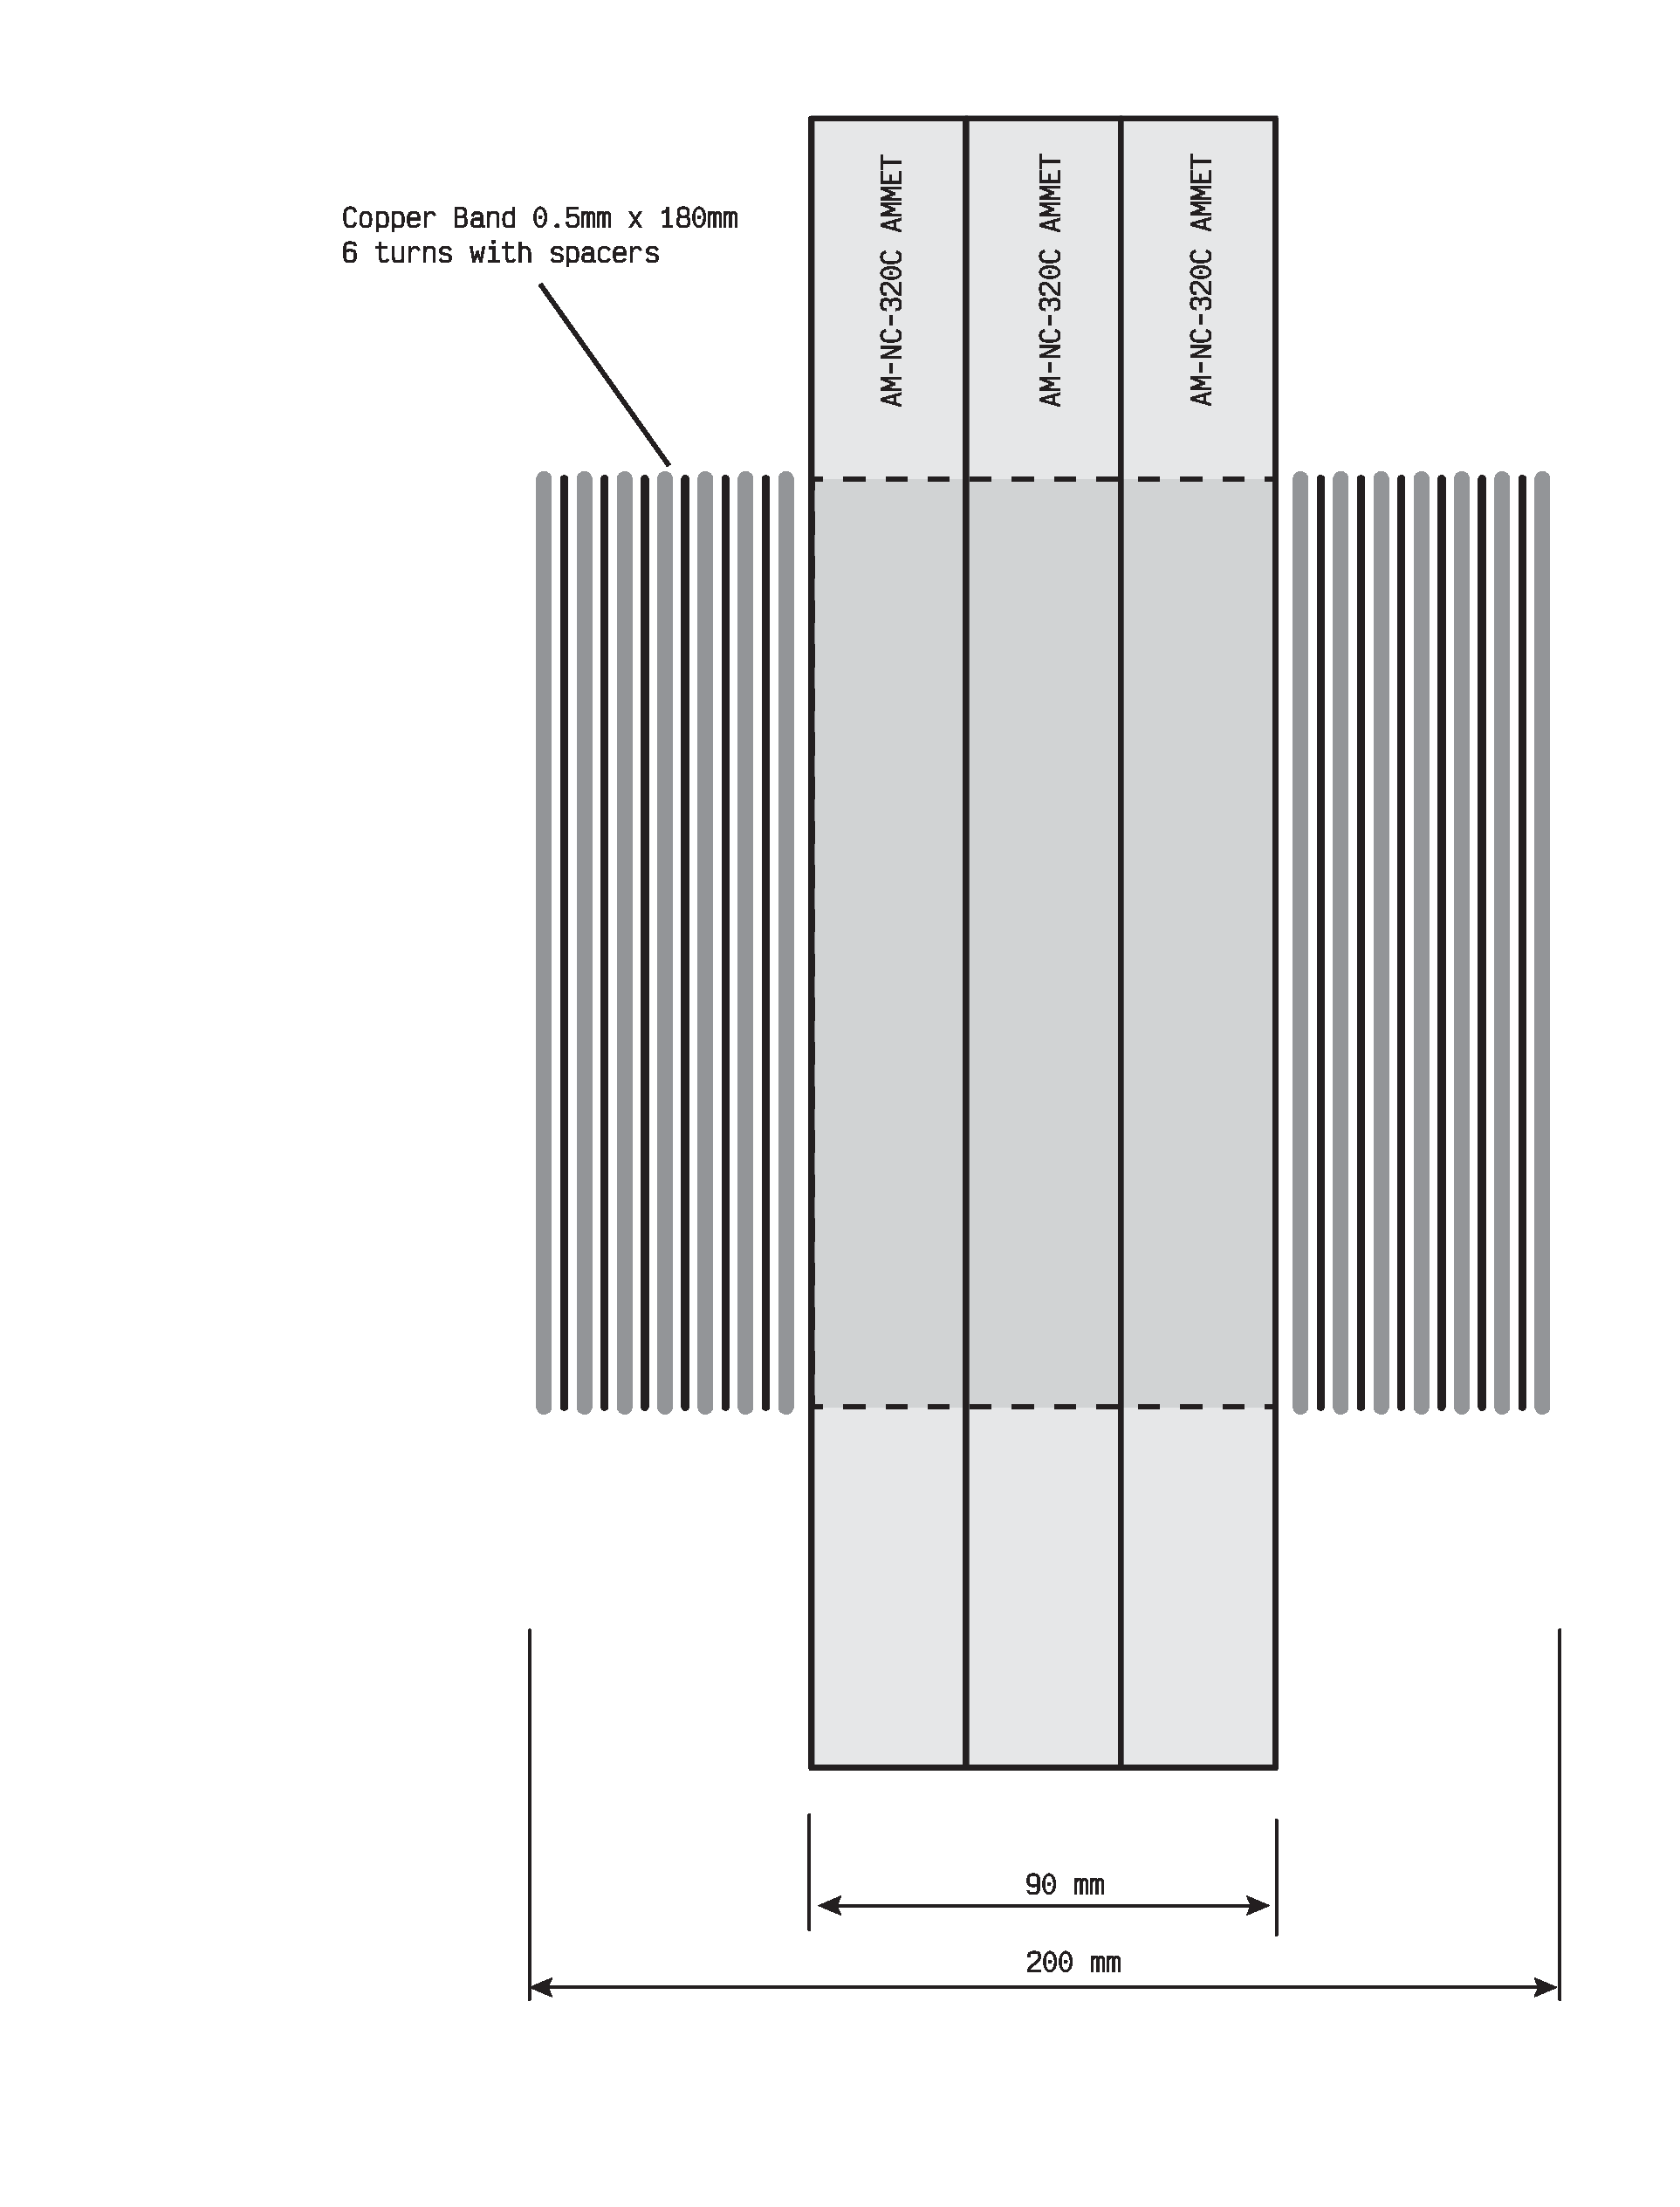
\includegraphics[width =250pt, angle = 0, 
		keepaspectratio]{figures/magnetics/three_phase_transformers_dab_6}
		\captionsetup{width=0.75\textwidth, font=footnotesize}	
		\caption{Single phase transformer for the three-phase DAB - side view.}
		\label{three_phase_transformers_dab_6}
	\end{subfigure}
	\captionsetup{width=0.65\textwidth, font=small}	
	\caption{Single phase transformer for the three-phase DAB.}
	\label{three_phase_transformers_dab_56}
\end{figure}

\subsection{Transformer design for 1P-DAB}

\noindent\textbf{Input data}:
\begin{itemize}
	\item[--] $u_1^{b} = \SI{800}{\volt} rms$: primary side nominal voltage;	
	\item[--] $u_2^{b} = \SI{800}{\volt} rms$: secondary side nominal voltage;	
	\item[--] $i_1^{b} = \SI{375}{\ampere} rms$: primary side nominal current;	
	\item[--] $i_2^{b} = \SI{375}{\volt} rms$: secondary side nominal current;
	\item[--] $f_{b} = \SI{12}{\kilo\hertz}$: fundamental frequency;
\end{itemize}

\noindent\textbf{Design}:
\begin{itemize}
	\item[--] core material: nanocrystalline alloy ($\mu_r = \SI{5000}{}$);	
	\item[--] core shape: C (AM-NC-412 AMMET);		
	\begin{itemize}
		\item[--] core height: $h_{fe} = \SI{290}{\milli\meter}$;	
		\item[--] core length: $L_{fe} = \SI{946}{\milli\meter}$;	
		\item[--] core width: $d_{fe} = \SI{60}{\milli\meter}$;		
		\item[--] core window: $W_{fe} = \SI{90}{\milli\meter}$;	
		\item[--] core depth: $D_{fe} = \SI{100}{\milli\meter}$;	
		\item[--] relative permeability $\mu_r = \SI{5000}{}$;
		\item[--] maximum magnetic flux density $\hat{B} = \SI{0.5}{\weber\per\square\meter}$;
	\end{itemize}
	\item[--] winding material: copper foil $d = \SI{0.5}{\milli\meter}$;		
	\item[--] winding current density: $J = \SI{3.0}{\ampere\per\square\milli\meter}$;	
\end{itemize}

\noindent calculus:
assuming $n_1 = n_2 = 6$
\begin{flalign}
	S_{fe} = 10^{4}\frac{u_1^{b}}{4.44\ f_b\ \hat{B}\ n_1} \approx \SI{50}{\square\centi\meter} &&
\end{flalign}
\begin{flalign}
	S_{cu} = \frac{i_1^{b}}{J} \approx \SI{125}{\square\milli\meter} &&
\end{flalign}
\begin{flalign}
	L_{cu} = \frac{S_{cu}}{d} \approx \SI{250}{\milli\meter} &&
\end{flalign}

\noindent\textbf{Remark} - core will be created using the nanocrystalline cut core AM-NC-412 by AMMET, that results in the following iron power losses: \\


\noindent\textbf{Specific Core Loss} 
\begin{flalign}
	P_{\mu} = \SI{16}{\watt\per\kilogram} \qquad \text{at}\quad f=\SI{4}{\kilo\hertz},\quad \hat{B}=\SI{0.8}{\weber\per\square\meter} &&
\end{flalign}
\noindent\textbf{Core mass}
\begin{flalign}
	m_{fe} = \SI{37}{\kilogram}&&
\end{flalign}
\noindent\textbf{Core power losses}
\begin{flalign}
	P_{fe} = \SI{593}{\watt} &&
\end{flalign}
\noindent\textbf{Copper power losses}
\begin{flalign}
	P_{cu} = \SI{67}{\watt} &&
\end{flalign}

\noindent\textbf{Total power losses}
\begin{flalign}
	P_{loss} = (P_{fe}+P_{cu}) = \SI{660}{\watt}&&
\end{flalign}

\begin{figure}[H]
	\centering
	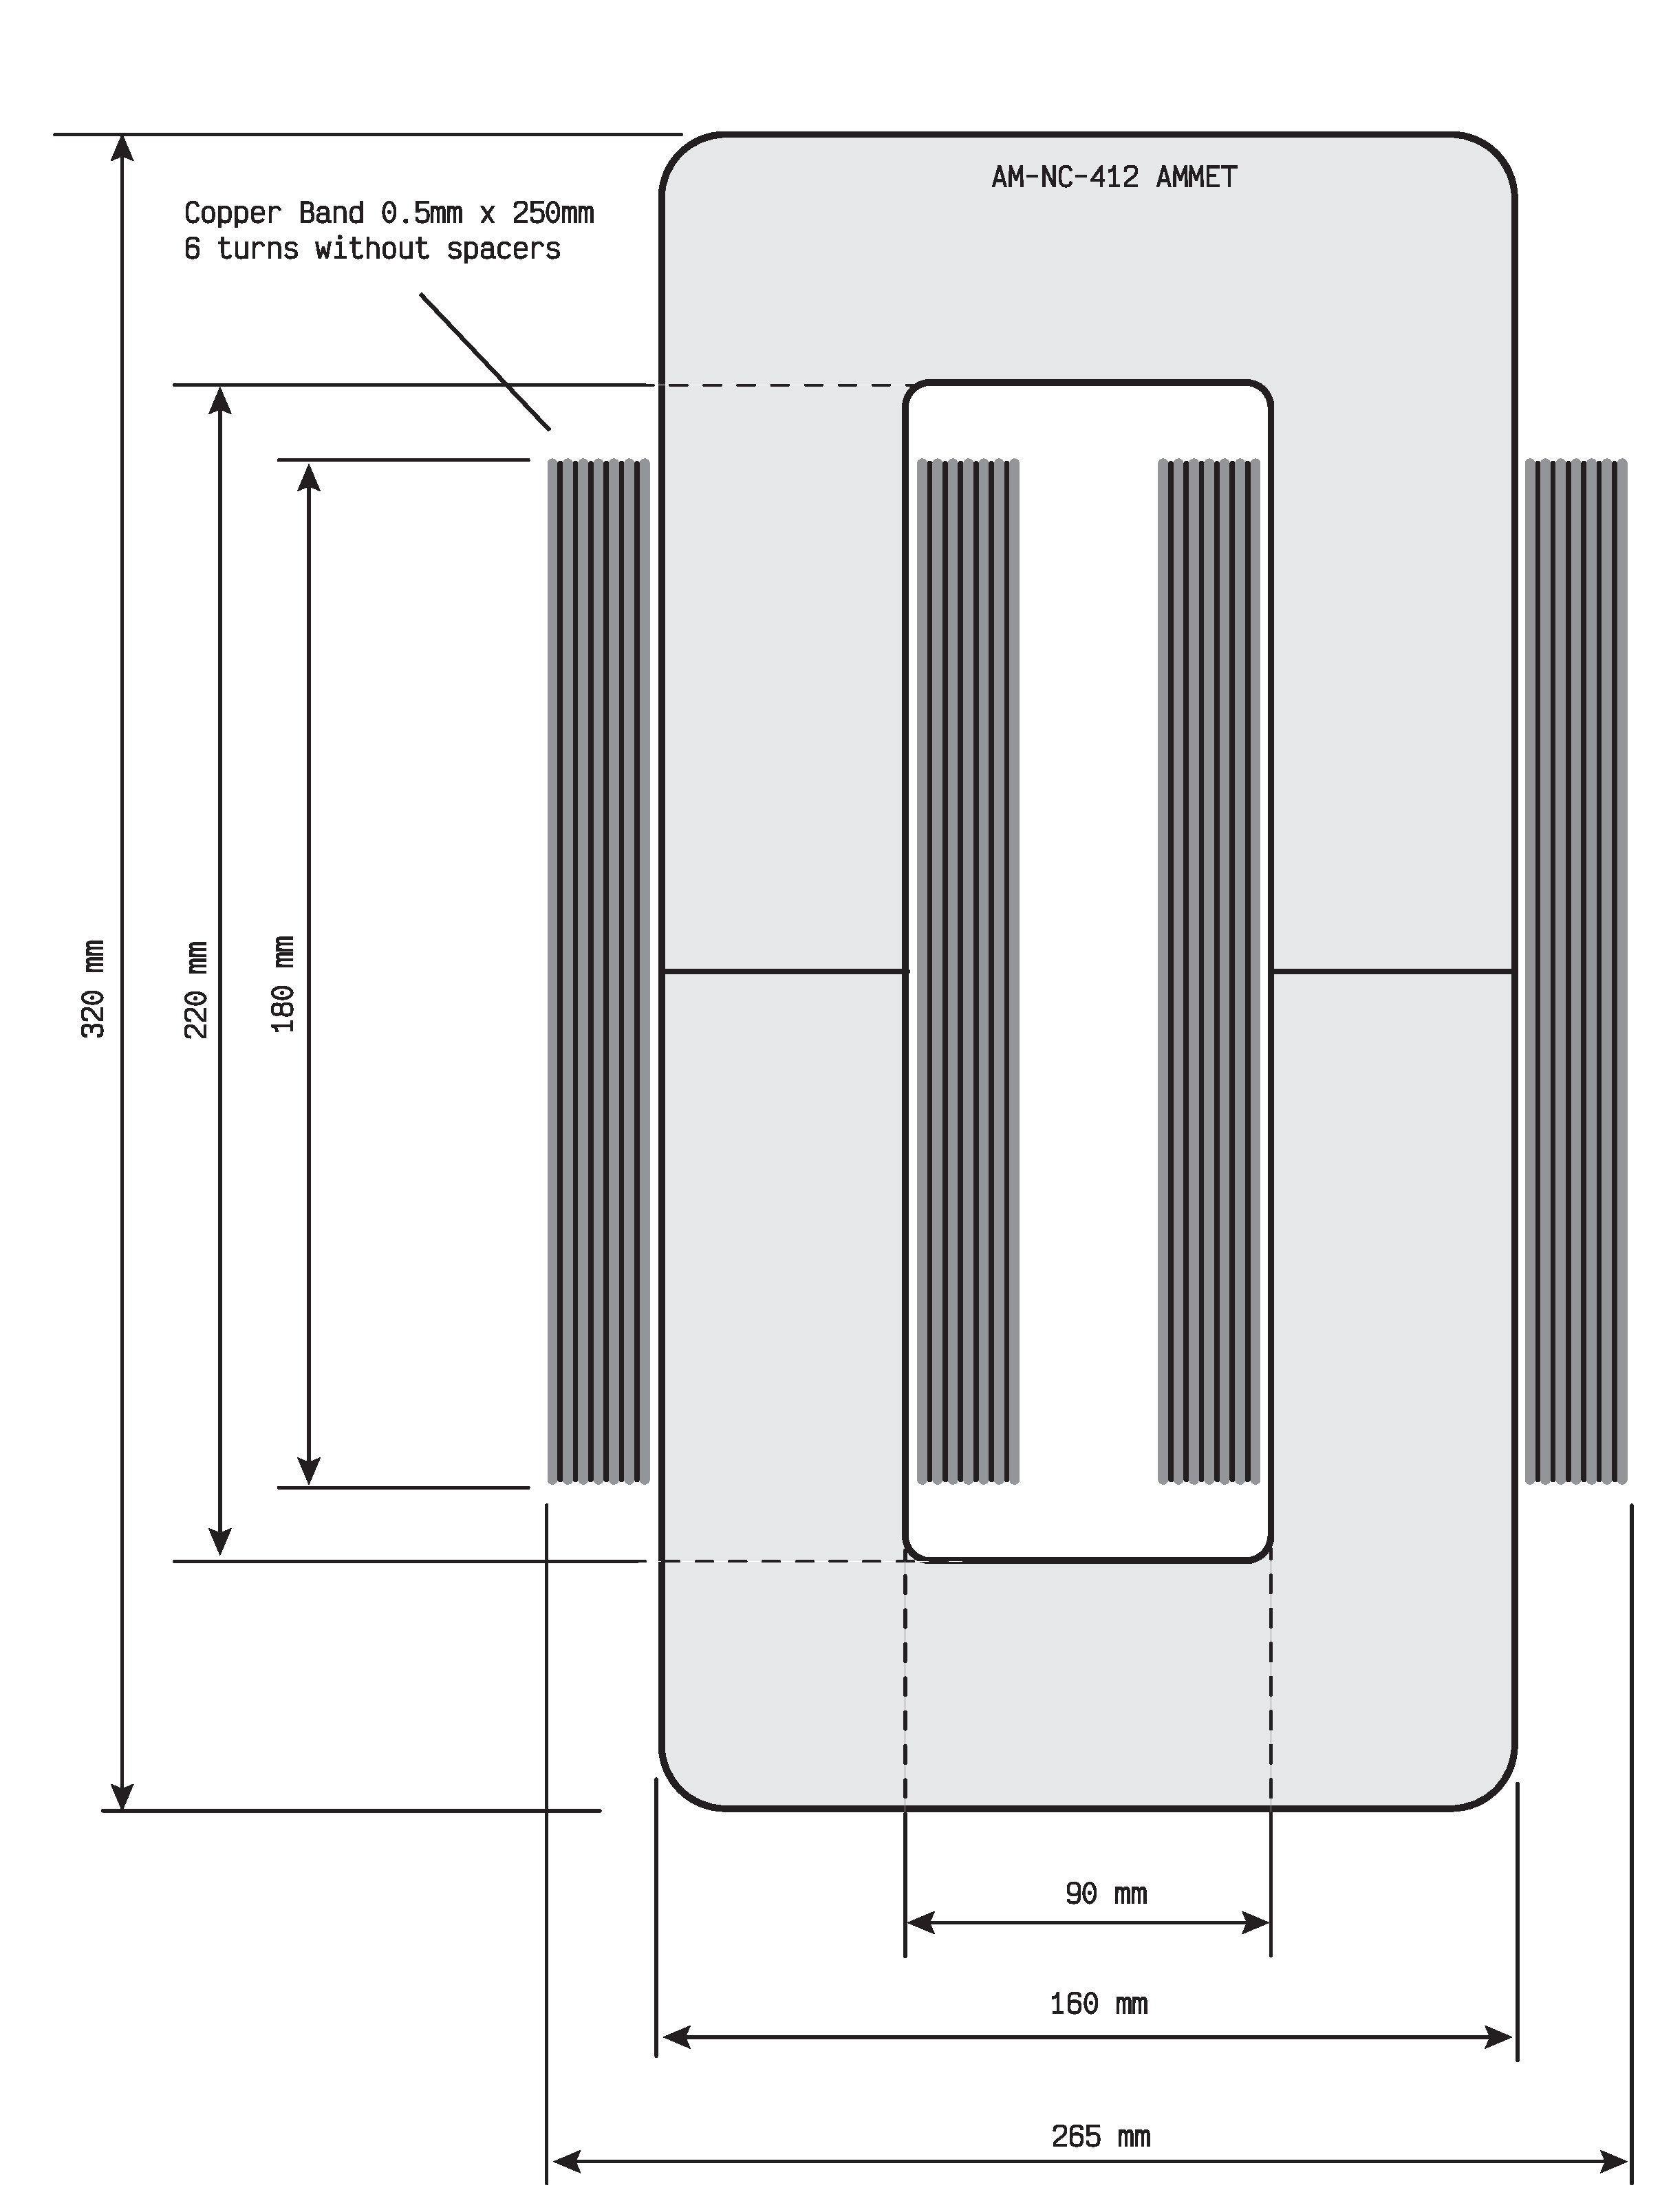
\includegraphics[width = 325pt, angle = 0, 
	keepaspectratio]{figures/magnetics/three_phase_transformers_dab_8}
	\captionsetup{width=0.5\textwidth, font=small}
	\caption{Transformer layout for the single-phase DAB - front view.}
	\label{three_phase_transformers_dab_8}
\end{figure}
\begin{figure}[H]
	\centering
	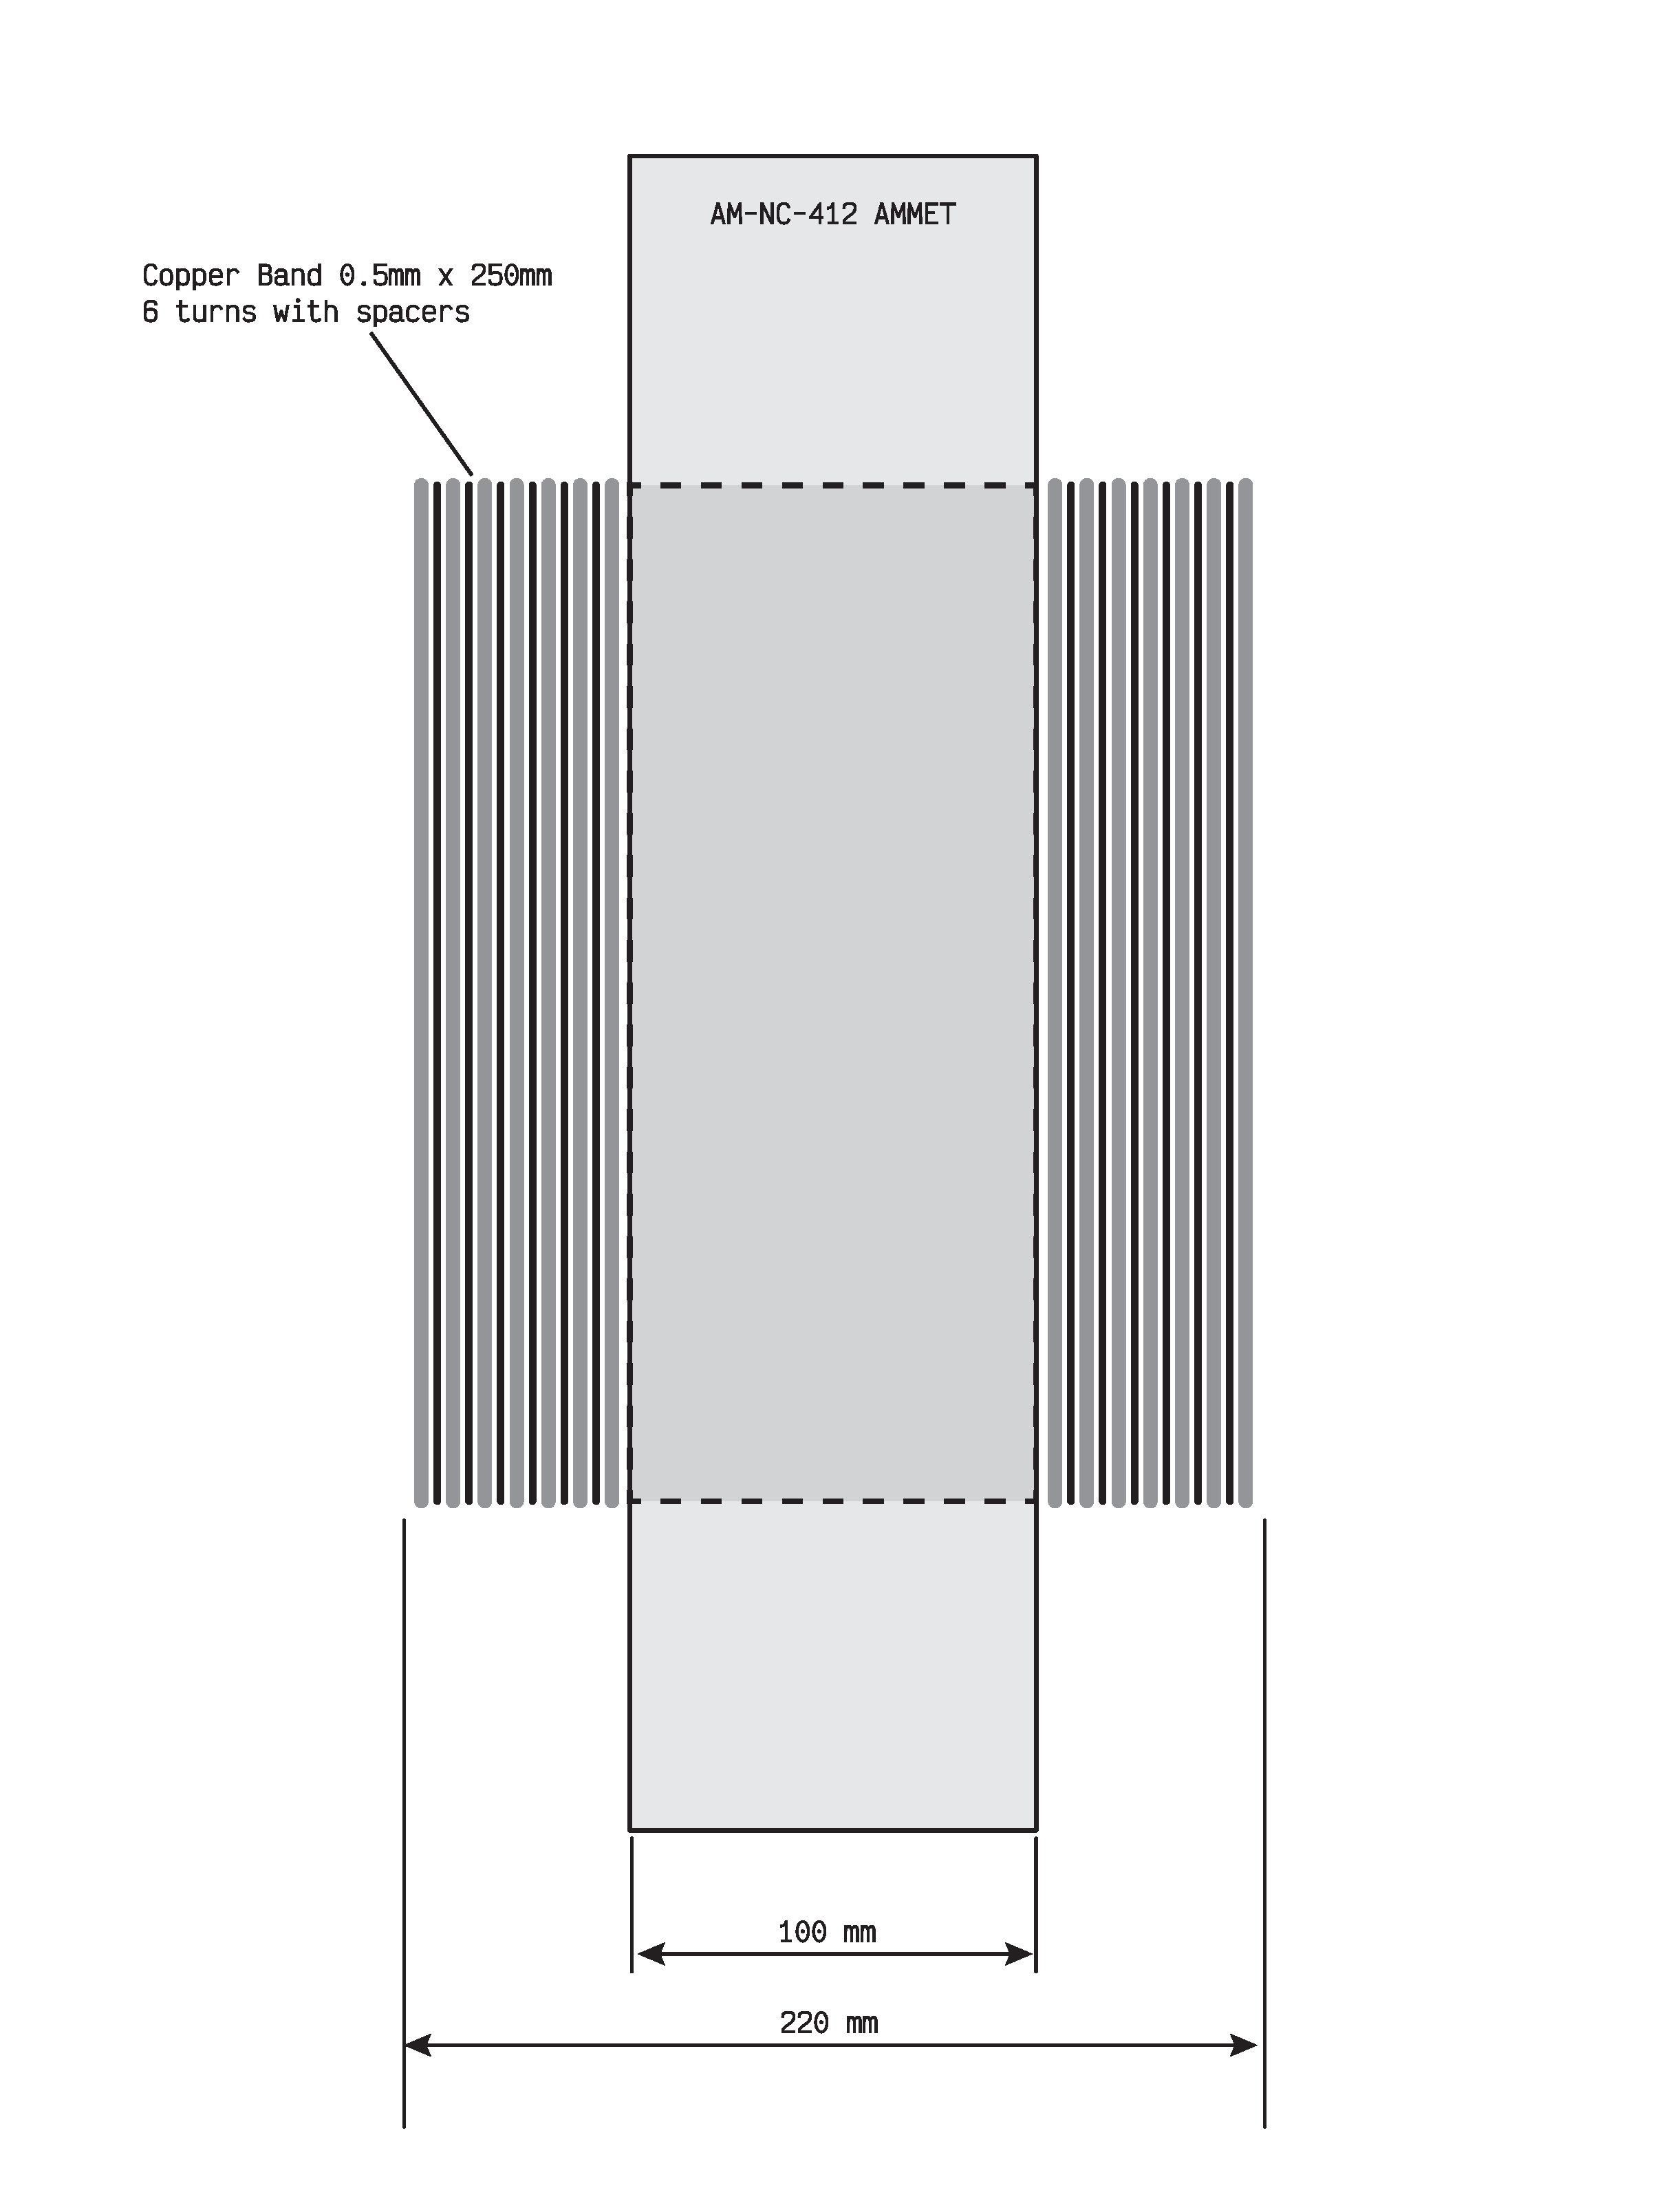
\includegraphics[width = 325pt, angle = 0, 
	keepaspectratio]{figures/magnetics/three_phase_transformers_dab_9}
	\captionsetup{width=0.5\textwidth, font=small}
	\caption{Transformer layout for the single-phase DAB - side view.}
	\label{three_phase_transformers_dab_9}
\end{figure}



\section{Summary of simulation results}
\label{sec:summary}
In this section a summary of overall efficiency for: three phase DAB,  single phase DAB, single phase CLLC is shown.

The power flow through each DC/DC/AC converter is around \SI{250}{kW}, in Table~\ref{summary_results_table_1} the total power loss concerning the semiconductors components are reported. Power loss concerning capacitors and inductors gave been not accounted at this stage.

\noindent\textbf{Remark} - T-Type single phase inverter will taken into account.
\begin{center}	
	\doublespacing
	\begin{longtable}{p{0.25\linewidth}|p{0.125\linewidth}|p{0.125\linewidth}|p{0.125\linewidth}|p{0.125\linewidth}}
		\captionsetup{width=0.65\textwidth, font=small}
		\caption{Comparison of power loss for three different DC/DC architecture.}
		\label{summary_results_table_1} \\
		\hline\hline
		\textbf{Architecture} & \hspace*{\fill} $f_{dab}\big[\SI{}{\kilo\hertz}\big]$  & \hspace*{\fill} $f_{inv}\big[\SI{}{\kilo\hertz}\big]$ & \hspace*{\fill} $p_{loss}^{dab}\big[\SI{}{\kilo\watt}\big]$  & \hspace*{\fill} $p_{loss}^{inv}\big[\SI{}{\kilo\watt}\big]$ \\
		\hline
		\textbf{Three phase DAB} & \hspace*{\fill} $\SI{4}{\kilo\hertz}$ & \hspace*{\fill} $\SI{4}{\kilo\hertz}$  & \hspace*{\fill} $\SI{2.27 }{\kilo\watt}$  & \hspace*{\fill} $\SI{3.0}{\kilo\watt}$  \\
		\hline
		\textbf{Single phase CLLC} & \hspace*{\fill} $\SI{13}{\kilo\hertz}$  & \hspace*{\fill} $\SI{4}{\kilo\hertz}$ & \hspace*{\fill} $\SI{2.25}{\kilo\watt}$  & \hspace*{\fill} $\SI{3.0}{\kilo\watt}$  \\
		\hline
		\textbf{Single phase DAB} & \hspace*{\fill} $\SI{12}{\kilo\hertz}$  & \hspace*{\fill} $\SI{4}{\kilo\hertz}$ & \hspace*{\fill} $\SI{1.28}{\kilo\watt}$  & \hspace*{\fill} $\SI{3.0}{\kilo\watt}$ \\
		\hline\hline
	\end{longtable}
\end{center}

From Table~\ref{summary_results_table_1} all solution seems promising until ZVS for single phase DAB or ZCS for CLLC are  satisfied. Impact into magnetic has to be investigated. 

In the following additional information are reported.
\begin{center}	
	\doublespacing
	\begin{longtable}{p{0.25\linewidth}|p{0.1\linewidth}|p{0.1\linewidth}|p{0.1\linewidth}|p{0.1\linewidth}|p{0.1\linewidth}|p{0.1\linewidth}}
		\captionsetup{width=0.65\textwidth, font=small}
		\caption{DC/DC transformers rms main quantities.}
		\label{transformers_data_design} \\
		\hline\hline
		\textbf{Architecture} & \hspace*{\fill} $f_{dab}\big[\SI{}{\hertz}\big]$  & \hspace*{\fill} $i_{1}\big[\SI{}{\ampere}_{rms}\big]$ & \hspace*{\fill}  $i_{2}\big[\SI{}{\ampere}_{rms}\big]$  & \hspace*{\fill}  $u_{1}\big[\SI{}{\volt}_{rms}\big]$ & \hspace*{\fill} $u_{2}\big[\SI{}{\volt}_{rms}\big]$ & \hspace*{\fill} $L_s\big[\SI{}{\henry}\big]$\\
		\hline
		\textbf{Single phase DAB} & \hspace*{\fill} $\SI{12}{\kilo\hertz}$ & \hspace*{\fill} $\SI{375}{\ampere}$  & \hspace*{\fill} $\SI{375}{\ampere}$  & \hspace*{\fill} $\SI{830}{\volt}$ & \hspace*{\fill} $\SI{752}{\volt}$ & \hspace*{\fill} $\SI{11}{\micro\henry}$\\
		\hline
		\textbf{Three phase DAB} & \hspace*{\fill} $\SI{4}{\kilo\hertz}$ & \hspace*{\fill} $\SI{265}{\ampere}$  & \hspace*{\fill} $\SI{265}{\ampere}$  & \hspace*{\fill} $\SI{400}{\volt}$ & \hspace*{\fill} $\SI{360}{\volt}$ & \hspace*{\fill} $\SI{28}{\micro\henry}$\\
		\hline
		\textbf{Single phase CLLC} & \hspace*{\fill} $\SI{13}{\kilo\hertz}$ & \hspace*{\fill} $\SI{452}{\ampere}$  & \hspace*{\fill} $\SI{452}{\ampere}$  & \hspace*{\fill} $\SI{815}{\volt}$ & \hspace*{\fill} $\SI{745}{\volt}$ & \hspace*{\fill} $\SI{13}{\micro\henry}$\\
		\hline\hline
	\end{longtable}
\end{center}

\noindent\textbf{Remark} - in Table~\ref{transformers_data_design} voltages for the three phase DAB represent the \textit{per phase} voltage and not the phase to phase, on the other hand voltages for the CLLC and single phase DAB architecture represent the voltage across the single phase transformer.

\noindent\textbf{Remark} - $L_s$  accounts also the leakage inductance of the transformer.

\noindent\textbf{Remark} - in summary, solution with single phase-DAB seems to be more effective in term of efficiency, even if stability under residual dc-current shall be investigated further.
   
\begin{center}	
	\doublespacing
	\begin{longtable}{p{0.25\linewidth}|p{0.12\linewidth}|p{0.12\linewidth}|p{0.12\linewidth}|p{0.12\linewidth}}
		\captionsetup{width=0.65\textwidth, font=small}
		\caption{Global efficiency using three phase DAB versus single phase DAB and T-Type single phase inverter assuming a power rate flow of $\SI{250}{\kilo\watt}$.}
		\label{global_efficiency} \\
		\hline\hline
		\textbf{Architecture} & \hspace*{\fill} $p_{loss}^{dab}\big[\SI{}{\kilo\watt}\big]$  & \hspace*{\fill} $p_{loss}^{tr}\big[\SI{}{\kilo\watt}\big]$ & \hspace*{\fill}  $p_{loss}^{inv}\big[\SI{}{\kilo\watt}\big]$ & \hspace*{\fill}  $\eta_{tot}\big[\SI{}{\percent}\big]$\\
		\hline
		\textbf{Single phase DAB} & \hspace*{\fill} $\SI{1.28}{\kilo\watt}$ & \hspace*{\fill} $\SI{0.66}{\kilo\watt}$  & \hspace*{\fill} $\SI{3.0}{\kilo\watt}$  & \hspace*{\fill} $\SI{98.0}{\percent}$ \\
		\hline
		\textbf{Three phase DAB} & \hspace*{\fill} $\SI{2.21}{\kilo\watt}$ & \hspace*{\fill} $\SI{0.86}{\kilo\watt}$  & \hspace*{\fill} $\SI{3.0}{\kilo\watt}$  & \hspace*{\fill} $\SI{97.6}{\percent}$ \\
		\hline\hline
	\end{longtable}
\end{center}


\section{SST bench based on the CLLC-DCX and the T-type inverter (2026)}
\label{sec:bench2026}
\setlength{\emergencystretch}{3em}
\renewcommand{\tabularxcolumn}[1]{>{\raggedright\arraybackslash}p{#1}}

\subsection{Architecture and numbers}
\label{sec:bench2026_arch}
The repository \cite{sst_repo} keeps today one bench of the SST, built on the outcome of the comparative study: a single phase CLLC used as a DC transformer for the isolated stage and the three level T-type bridge for the inverter, at \SI{50}{\kilo\watt} per module. Two modules are modelled (Figure~\ref{fig:bench2026}): two lithium-ion packs in parallel on the \SI{800}{\volt} battery bus, one CLLC-DCX per module (\SI{800}{\volt} to \SI{800}{\volt}, $11:11$, \SI{50}{\kilo\hertz}, open loop, Wolfspeed CAB006M12GM3 SiC modules on both bridges), one T-type single phase inverter per module on the isolated \SI{800}{\volt} DC link, the two inverters in series on a single phase line of $2 \times \SI{398.4}{\volt}$ rms. Module A runs the current loop, module B applies the same modulation vector with its own PLL angle, which is the master/slave arrangement of Section~\ref{sec:global_arch} reduced to two units. Table~\ref{tab:bench2026} collects the numbers of the bench; they are in the parameter file \texttt{private/sst\_cllc\_ttype\_param.m} of the bench folder, and those of the DCX in the library file \texttt{cllc\_dcx\_param\_example.m}. The sizing of the DCX is the subject of \cite{cllc_dcx_doc}, the design of the inverter control of \cite{spinv_doc}: this section describes the bench, the models and their organization.

\begin{figure}[H]
	\centering
	\begin{tikzpicture}[font=\footnotesize, >=Latex,
		blk/.style={draw, thick, rounded corners=2pt, minimum height=1.3cm, minimum width=2.6cm, align=center, fill=blue!4},
		dcx/.style={draw, thick, rounded corners=2pt, minimum height=1.3cm, minimum width=2.6cm, align=center, fill=orange!12},
		src/.style={draw, thick, rounded corners=2pt, minimum height=1.3cm, minimum width=2.2cm, align=center, fill=gray!8, dashed}]
		\node[src] (bat1) at (0,1.2) {battery pack 1\\\SI{800}{\volt}, \SI{50}{\kilo\watt}};
		\node[src] (bat2) at (0,-1.2) {battery pack 2\\\SI{800}{\volt}, \SI{50}{\kilo\watt}};
		\node[dcx] (dcx1) at (4.0,1.2) {CLLC-DCX 1\\\SI{800}{\volt} / \SI{800}{\volt}\\\SI{50}{\kilo\hertz}, open loop};
		\node[dcx] (dcx2) at (4.0,-1.2) {CLLC-DCX 2\\\SI{800}{\volt} / \SI{800}{\volt}\\\SI{50}{\kilo\hertz}, open loop};
		\node[blk] (inv1) at (8.2,1.2) {T-type inverter A\\\SI{800}{\volt} link, \SI{4}{\kilo\hertz}\\master: PLL, dq PI};
		\node[blk] (inv2) at (8.2,-1.2) {T-type inverter B\\\SI{800}{\volt} link, \SI{4}{\kilo\hertz}\\slave of A};
		\node[src, minimum height=3.4cm, minimum width=1.9cm] (line) at (12.0,0) {line\\$2 \times \SI{398}{\volt}$\\rms, \SI{50}{\hertz}\\\SI{0.5}{\milli\henry}\\per inductor};
		% DC bus
		\draw[thick] (bat1) -- (dcx1); \draw[thick] (bat2) -- (dcx2);
		\draw[thick] (1.9,1.2) -- (1.9,-1.2);
		\node[font=\scriptsize, anchor=west] at (2.0,0) {\SI{800}{\volt} bus};
		% isolated links
		\draw[thick] (dcx1) -- (inv1) node[midway, above, font=\scriptsize] {side 2}; \draw[thick] (dcx2) -- (inv2) node[midway, above, font=\scriptsize] {side 2};
		% series connection on the AC side
		\draw[thick] (inv1.east) -- ++(0.7,0) |- (line.north west);
		\draw[thick] (inv2.east) -- ++(0.7,0) |- (line.south west);
		\draw[thick] ([yshift=-0.35cm]inv1.east) -- ++(0.35,0) |- ([yshift=0.35cm]inv2.east);
		% sync
		\draw[->, thick, dashed, blue!60!black] (inv1.south) -- (inv2.north) node[midway, left, font=\scriptsize, align=right] {sync:\\$\theta$, $m_d$, $m_q$};
	\end{tikzpicture}
	\captionsetup{width=0.85\textwidth, font=small}
	\caption[Two-module SST bench of the repository (2026).]{Two-module SST bench of the repository (2026): two battery packs on the \SI{800}{\volt} bus, one CLLC-DCX and one T-type inverter per module, the inverters in series on the line; module B is the slave of module A.}
	\label{fig:bench2026}
\end{figure}

\begin{table}[H]
	\centering
	\captionsetup{width=0.9\textwidth, font=small}
	\caption[Numbers of the two-module bench.]{Numbers of the two-module bench (\texttt{private/sst\_cllc\_ttype\_param.m}, DCX from \texttt{cllc\_dcx\_param\_example.m}).}
	\label{tab:bench2026}
	\rowcolors{2}{tableShade}{white}
	\small
	\begin{tabularx}{0.97\textwidth}{@{} >{\raggedright\arraybackslash}p{0.24\textwidth} X @{}}
		\toprule
		\textbf{Item} & \textbf{Value} \\
		\midrule
		Modules & 2, DC sides in parallel, AC sides in series, \SI{50}{\kilo\watt} each (\SI{100}{\kilo\watt} in total) \\
		Battery bus & 2 packs $\times$ \SI{800}{\volt}, \SI{50}{\kilo\watt}, \SI{62.5}{\ampere\hour} (1C), SOC 0.85; the pack resistances halved and the time constant of the RC branch shortened for the run \\
		DCX, per module & \SI{800}{\volt} to \SI{800}{\volt} ($11:11$), \SI{62.5}{\ampere}, $f_s = \SI{50}{\kilo\hertz}$ at $f_n = 0.95$ ($f_r = \SI{52.6}{\kilo\hertz}$), $L_r = \SI{12}{\micro\henry}$, $C_r = \SI{0.762}{\micro\farad}$ per side, $L_m = \SI{400}{\micro\henry}$, dead time \SI{300}{\nano\second}; mode 0: bridge 1 PWM at \SI{50}{\percent}, bridge 2 synchronous rectifier; DC chokes \SI{250}{\micro\henry}, DC-link capacitor of side 1 \SI{500}{\micro\farad}, side 2 left to the inverter block \\
		Inverter, per module & $u_{dc} = \SI{800}{\volt}$, $u_{bez} = 0.9\,u_{dc} = \SI{720}{\volt}$, $i_{s}^{nom} = \SI{125.5}{\ampere}$ rms, $f_{pwm} = \SI{4}{\kilo\hertz}$ with double update ($t_s = \SI{125}{\micro\second}$), dead time \SI{300}{\nano\second}, split DC link $C_{Fi} = \SI{3}{\milli\farad}$ ($2 \times \SI{6}{\milli\farad}$ in series), $L_{Fu} = \SI{500}{\micro\henry}$ (two halves), $C_{Fu} = \SI{50}{\micro\farad}$ with \SI{50}{\milli\ohm}, Wolfspeed CAB006M12GM3 \\
		Line & $690/\sqrt{3} = \SI{398.4}{\volt}$ rms per module (\SI{563.4}{\volt} peak), \SI{796.7}{\volt} rms in total, \SI{50}{\hertz}, two line inductors of \SI{0.5}{\milli\henry} and \SI{10}{\milli\ohm} (\SI{5}{\percent}) \\
		Control & module A: single phase PLL on the line voltage, first harmonic tracker on the current, dq vector PI; module B: slave, applies $m_d$, $m_q$ of A with its own PLL angle. Gains kp \num{0.5} / ki \num{45} in the discrete model, kp \num{0.1} / ki \num{20} in the compact one (Section~\ref{sec:bench2026_ctrl}); reference \SI{1}{pu} from \SI{0.35}{\second} with a slew of \SI{2}{pu/s}; gates of the compact modules enabled at \SI{0.1}{\second}, after the PLL has locked \\
		Run & \SI{1.25}{\second}, Backward Euler local solver at $t_c = \SI{100}{\nano\second}$ (\SI{1}{\micro\second} for quick runs), the last \SI{0.2}{\second} logged at $t_c$ \\
		\bottomrule
	\end{tabularx}
	\rowcolors{1}{white}{white}
\end{table}

\subsection{Control}
\label{sec:bench2026_ctrl}
The DCX stages run in open loop (mode 0 of the library block): the isolated DC links follow the battery bus through the $1:1$ transformer minus the drop on an equivalent resistance of about \SI{43}{\milli\ohm}, and the power is set by the inverters, as explained in Section~\ref{sec:control_arch} and in \cite{cllc_dcx_doc}. The control of the bench is therefore the control of the inverters, which is the single phase chain of Section~\ref{sec:control_arch} in its virtual vector form: a single phase PLL on the terminal voltage (Park PLL with the virtual quadrature component and a double integrator observer that gives the angle of the control), a first harmonic tracker on the line current that provides its fundamental and quadrature components, the dq vector PI with the clip flag and the integrator release, the DC-link voltage feed-forward and the vector-length limiter, and the three level modulators of the two legs with the dead time around both edges. Module A closes the loop; module B reads the angle and the modulation vector of A through the \texttt{sync} link and applies them with its own PLL angle, so that two identical modules in series produce the same voltage and carry the same current. The design of these loops, the discrete implementation and their verification on the model are the subject of \cite{spinv_doc}.

The gains deserve a remark, because the two models of the bench use different values. The discrete model keeps the gains of the 2025 study, $k_p = 0.5$ and $k_i = \SI{45}{1/s}$ at $t_s = \SI{125}{\micro\second}$. With the first harmonic tracker in the feedback path and the resonance of the output filter at about \SI{1.4}{\kilo\hertz} ($L_{Fu} = \SI{500}{\micro\henry}$, $C_{Fu} = \SI{50}{\micro\farad}$), the open-loop response of the compact block (PI, one-step acquisition delay, zero-order-hold plant, tracker) has \ang{15} of phase margin at \SI{1.7}{krad/s} and a loop gain of \num{1.9} at the resonance with these values, and the time-domain run is unstable; $k_p = 0.1$ and $k_i = \SI{20}{1/s}$ give a crossover at \SI{510}{rad/s} with \ang{53} of phase margin and \num{0.37} at the resonance, and are the values of the compact modules (\texttt{kp\_i}, \texttt{ki\_i} of the parameter file). The analysis is in the header of \path{afe_single_phase_ttype_param_example.m} of the library and in \cite{spinv_doc}.

\subsection{The two models}
\label{sec:bench2026_models}
The bench folder (\path{theory_analysis_solid_state_transformer/sst_based_on_full_bridge_ttype_inverter/sst_single_phase_cllc_single_phase_ttype_inv}) holds two models of the same bench, which share the initialization, the parameters and the post-processing scripts; \texttt{param.sim.model} in \texttt{init\_model.m} chooses the one to open and simulate:

\begin{itemize}[nosep]
	\item \texttt{sst\_cllc\_ttype\_inv.slx}, the \textbf{compact} model: the T-type modules are two instances of the library block \path{afe_single_phase_ttype_mod1} in the wrappers \path{single_phase_inverter_modA_cmp} and \path{modB_cmp} (mask parameters \texttt{param.spinv.p\_modA} and \texttt{p\_modB}, the sync link from A to B inside the wrappers), the DCX stages are two instances of \texttt{cllc\_dcx\_mod1} (\texttt{param.cllc.p\_mod1}, \texttt{p\_mod2}). The switches of both blocks are numerical with the conduction drop only: no switching losses, no thermal model. It is the model for the control studies and for long runs;
	\item \texttt{sst\_cllc\_ttype\_inv\_discrete.slx}, the \textbf{discrete} model: the T-type modules \path{single_phase_inverter_modA/B} are built from the discrete blocks of the library (\texttt{dclink} block, output filter, the T-type bridge \path{mosfet_based_three_level_inverter_ttype} with its thermal model, the control subsystem with the dq vector PI), module B applying the voltage command of A; the DCX stages are the same library blocks. The switch losses and the device temperatures (\path{mosfet_ploss_invQ1..4_sim}, device scopes) exist in this model only.
\end{itemize}

\noindent The root of both models has the two batteries (library block \texttt{lithium\_ion\_battery}; one Solver Configuration in the model, in \texttt{line\_source}, because the DCX blocks connect the two sides in one physical network), the two DCX wrappers, the \texttt{global timing} block with the master time and the local times of the modules, the \texttt{line\_source} with the two controlled voltage sources and the line inductors, the scopes and the \texttt{storage\_data\_sst} subsystem that logs every \texttt{*\_sim} signal at $t_c$ over the last \SI{0.2}{\second}. The log names are the same in the two models, so \texttt{power\_loss\_calculus.m} (battery, DCX, inverter and line powers, losses and efficiency over the last five grid periods, with the Backward Euler estimate of the tank damping), \texttt{plotting\_results.m} and \texttt{spectrum.m} (spectra and THD of the line current) work on either run. The script that converted the 2025 model to the library blocks is archived in \texttt{legacy/}.

\subsection{The library blocks}
\label{sec:bench2026_blocks}
The MATLAB Home licence used for the project limits a model to 1000 nonvirtual blocks, referenced models and library links included, and the 2025 models were above that with two modules. Two blocks of \cite{library_repo} solve it, each one modelling a complete converter with two nonvirtual blocks: a Simscape language component for the power stage and one MATLAB Function, discrete at the step of the local solver, for the modulator and the control. Both follow the same conventions: one structure \texttt{p} on the mask (\texttt{p.hw} the parameters of the component, \texttt{p.pwm} the carrier and the gates, \texttt{p.ctrl} the control), the input \texttt{t\_master} for the master time of the model, the output \texttt{m} with the measurements in pu and the output \texttt{ctrl\_log} with the control signals, whose indices are returned by name by a companion function; the control reads the measurements one step behind through a Unit Delay, the DC quantities as averages over the control period, quantized as an ADC would.

\begin{itemize}[nosep]
	\item \texttt{cllc\_dcx/cllc\_dcx\_mod1}: ports \texttt{dc1+}, \texttt{dc1-} on the left and \texttt{dc2+}, \texttt{dc2-} on the right, galvanically separate (one Electrical Reference per side in the model); \texttt{m} [15$\times$1] (DC voltages and currents of both sides, tank currents, bridge and capacitor voltages, DC buses, magnetizing and capacitor currents) and \texttt{ctrl\_log} [24$\times$1]; modes 0 open-loop DCX, 1 current loop, 2 voltage loop; each bridge in PWM, synchronous rectifier or off; optional soft start, DC links and chokes. Fully described in \cite{cllc_dcx_doc};
	\item \texttt{afe\_single\_phase\_ttype/afe\_single\_phase\_ttype\_mod1}: ports \texttt{a}, \texttt{b} on the left (AC terminals after the LC filter) and \texttt{dc+}, \texttt{dc-} on the right (split DC link with its neutral point inside); inputs \texttt{t\_master} and \texttt{sync}, outputs \texttt{m} [13$\times$1] (converter and terminal currents, terminal and bridge voltages, DC link and its halves, DC and neutral currents, bank and filter currents), \texttt{ctrl\_log} [32$\times$1] and \texttt{sync\_out} = $[\hat\theta;\, m_d;\, m_q]$; \texttt{p.ctrl.mode} 0 current references (with step time and slew), 1 DC-link voltage loop; \texttt{p.ctrl.slave} = 1 applies the modulation vector of the block wired to \texttt{sync}; optional enable time and Gaussian noise on the current sample. Described with its control design in \cite{spinv_doc}.
\end{itemize}

\noindent Each block is built from its sources by a script of its folder (\path{update_cllc_dcx.m}, \path{update_afe_single_phase_ttype.m}) once the Simscape component has been compiled with \texttt{ssc\_build} from \path{library/foundation/pwr_electronics}; the example parameter files of the two folders (\path{cllc_dcx_param_example.m}, \path{afe_single_phase_ttype_param_example.m}) are the parameter sets of this bench, which the setup script of the bench reads and completes with its own numbers.

\subsection{Parameter structure}
\label{sec:bench2026_param}
The models read one structure, \texttt{param}, with one group per subsystem (Table~\ref{tab:param2026}). \texttt{init\_model.m} holds the simulation settings only (\texttt{param.sim}: model, run length, step, nonlinear iterations, export of the legacy names), puts the companion library on the path through \texttt{private/library\_setup.m} (the copy already on the path, else the folder \texttt{library} next to the repository or the one named by the environment variable \texttt{PWR\_CONTROL\_LIBRARY}, cloned from GitHub when missing) and calls \texttt{private/sst\_cllc\_ttype\_setup.m}, which builds the rest of \texttt{param} from the numbers of \texttt{private/sst\_cllc\_ttype\_param.m} and from the example files of the library (the timing object, the mask structures of the four blocks, the inverter hardware and control objects of the discrete model, the batteries, the heatsink). The post-processing scripts read \texttt{param.*} only. While \texttt{param.sim.export\_legacy\_names} is set, \texttt{private/sst\_cllc\_ttype\_legacy.m} also puts in the base workspace the flat names that the discrete model still reads; the migration of the model to \texttt{param.*} is the last step left of the conversion.

\begin{table}[H]
	\centering
	\captionsetup{width=0.9\textwidth, font=small}
	\caption[Groups of the structure \texttt{param} of the bench.]{Groups of the structure \texttt{param} of the bench (\texttt{init\_model.m} and \texttt{private/sst\_cllc\_ttype\_setup.m}).}
	\label{tab:param2026}
	\rowcolors{2}{tableShade}{white}
	\small
	\begin{tabularx}{0.97\textwidth}{@{} l X @{}}
		\toprule
		\textbf{Group} & \textbf{Content} \\
		\midrule
		\texttt{param.sim} & \texttt{model} (compact or discrete), \texttt{simlength}, \texttt{tc}, \texttt{nonlinear\_iterations}, \texttt{export\_legacy\_names} \\
		\texttt{param.time}, \texttt{.glb\_time} & inputs of the timing object (carrier, double update, dead time, logged window, battery sample time) and the object itself (\texttt{timing\_setup}): \texttt{tc}, \texttt{ts\_inv}, carriers and TRGO of the modulators \\
		\texttt{param.sst} & number of modules, power per module and in total \\
		\texttt{param.grid} & line: voltage per module and in total, frequency, line inductance and resistance \\
		\texttt{param.cllc} & operating point of the DCX stage, \texttt{mode}, \texttt{interleave}; \texttt{p\_mod1}, \texttt{p\_mod2} mask structures of the two DCX blocks; \texttt{idx} indices of their control log \\
		\texttt{param.spinv} & T-type inverter of one module (both modules read it): \texttt{hw\_in}/\texttt{hw}, \texttt{ctrl\_in}/\texttt{ctrl}, \texttt{sogi}, \texttt{mosfet}, \texttt{ideal\_switch}, references (\texttt{i\_ref}, \texttt{t\_ref}, \texttt{i\_ref\_slew}); \texttt{p\_modA}, \texttt{p\_modB} mask structures of the compact modules (B slave of A), \texttt{idx}, and the gains that rebuild the old log signals in physical units from \texttt{m} \\
		\texttt{param.ctrl} & \texttt{clip\_release} of the PI blocks of the discrete model \\
		\texttt{param.battery} & the two packs (\texttt{pack\_1}, \texttt{pack\_2}) \\
		\texttt{param.meas}, \texttt{.thermal}, \texttt{.dev} & ADC quantization; heatsink of the discrete model; names of the device datasets \\
		\bottomrule
	\end{tabularx}
	\rowcolors{1}{white}{white}
\end{table}

\subsection{Timing and numerical settings}
\label{sec:bench2026_num}
Each converter runs on its own local time base (\texttt{time\_master}, \texttt{time\_afe\_module\_A/B}, \texttt{time\_cllc\_module\_A/B} in the models, the local clock inside the library blocks): the modulators generate the control triggers from their carriers, and the local clocks can be detuned to study the effect of time sliding between modules. The inverters switch at \SI{4}{\kilo\hertz} with the control at $2 f_{pwm}$ (double update, $t_s = \SI{125}{\micro\second}$); the DCX blocks run at the step of the model, and their carriers can be interleaved by a quarter of the switching period (\texttt{param.cllc.interleave}, off by default) so that the $2 f_s$ ripple currents of the two stages cancel on the battery bus.

The whole physical network runs on the Simscape local solver with the Backward Euler method and the fixed step \texttt{param.sim.tc}, which must divide $t_s$. The method adds to each resonant tank a series resistance proportional to the step, about $2\,(\omega_s^2 L_{r1} t_c/2 + t_c/(2 C_{r1}))$ referred to side 1: \SI{2.5}{\ohm} at \SI{1}{\micro\second}, \SI{0.25}{\ohm} at \SI{100}{\nano\second}, \SI{0.125}{\ohm} at \SI{50}{\nano\second}, to be compared with the \SI{43}{\milli\ohm} of the physical stage. At \SI{1}{\micro\second} (20 steps per DCX period, the dead times shorter than one step) the damping takes about \SI{12}{\kilo\watt} per module at full load and lowers the isolated DC link by some \SI{150}{\volt}: that step is good for structural checks and for the grid-side loops only, and \texttt{power\_loss\_calculus.m} prints the estimate next to the measured DCX losses. The bench uses \SI{100}{\nano\second} (run time about ten times longer); \SI{50}{\nano\second} is the step of the DCX bench for the voltages, the losses and the ZVS, see \cite{cllc_dcx_doc}. \texttt{param.sim.nonlinear\_iterations} = 5 is needed by the thermal switch models of the discrete model.

\subsection{How to run and open points}
\label{sec:bench2026_run}
Run \texttt{init\_model.m} in the bench folder (it builds \texttt{param}, opens the model chosen by \texttt{param.sim.model} and prints the operating point), simulate \SI{1.25}{\second} (the DC links start at their nominal voltage, the current reference steps at \SI{0.35}{\second} and ramps to \SI{1}{pu} in \SI{0.5}{\second}), then \path{power_loss_calculus.m}, \path{plotting_results.m} and \path{spectrum.m}; \path{non_virtual_blocks_counting.m} checks the block count against the licence limit. Runs are saved with the \texttt{*\_sim} logs and \texttt{param} in a \texttt{.mat} file ignored by git. No run of the bench is saved in the repository at the time of this revision, and the results of the first ones (currents and voltages of both stages, efficiency chain from the batteries to the line, spectrum of the line current, device losses and temperatures of the discrete model) are to be added here. The open points are those of the two notes: the sizing checks of the DCX \cite{cllc_dcx_doc}, the tuning and the verification of the inverter loops on the complete bench \cite{spinv_doc}, the placeholders marked TBC in the parameter file (DC-link bank, filter, line impedance, devices) and the migration of the discrete model to \texttt{param.*}.

\begin{thebibliography}{99}
	\bibitem{dedonker1}
	R. De Doncker, D. M. Divan, M. H. Kheraluwala \emph{A Three-phase Soft-Switched High-Power-Density dc /dc Converter for High-Power Applications}. Transactions of Industry Applications vol. 27 No. 1 January 1991.

	\bibitem{akagi1} 
	H. Akagi, S. Kinouchi, Y. Miyazaki \emph{Bidirectional Isolated Dual-Active-Bridge (DAB) DC-DC Converters Using 1.2-kV 400-A SiC-MOSFET Dual Modules}. Transactions of Power Electronics vol. 1 No. 1 December 2016.

	\bibitem{krismer} 
	F. Krismer, \emph{Modeling and Optimization of Bidirectional Dual Active Bridge DC–DC Converter Topologies}. PhD dissertation, 2010.

	\bibitem{liserre}
	R. Teodorescu, M. Liserre, P. Rodrıguez, \emph{Grid converters for photovoltaic and wind power systems}. Wiley, 2011.

	\bibitem{cllc_dcx_doc}
	D. Bagnara, \emph{CLLC-DCX isolated DC/DC stage: 800 V / 800 V, 50 kW, 50 kHz, sizing, simulation model and library block}. pwr-control technical design note, Rev. 00, October 2026, \texttt{repos\_doc/cllc\_dcx} of \url{https://github.com/pwr-control/repositories-documentation}.

	\bibitem{spinv_doc}
	D. Bagnara, \emph{Single-Phase Grid-Tied T-Type Inverter: model, control design and discrete implementation}. pwr-control technical report, October 2026, \texttt{repos\_doc/single\_phase\_grid\_tied\_inverter\_analysis} of \url{https://github.com/pwr-control/repositories-documentation}.

	\bibitem{sst_repo}
	pwr-control, \emph{solid-state-transformers} repository, \url{https://github.com/pwr-control/solid-state-transformers}.

	\bibitem{library_repo}
	pwr-control, \emph{library} repository (Simscape components, masked blocks, setup classes and documentation), \url{https://github.com/pwr-control/library}.
\end{thebibliography}

\end{onehalfspace}
\end{document} 